%%
% The BIThesis Template for Bachelor Graduation Thesis
%
% 北京理工大学毕业设计(论文) —— 使用 XeLaTeX 编译
%
% Copyright 2021-2023 BITNP
%
% This work may be distributed and/or modified under the
% conditions of the LaTeX Project Public License, either version 1.3
% of this license or (at your option) any later version.
% The latest version of this license is in
%   http://www.latex-project.org/lppl.txt
% and version 1.3 or later is part of all distributions of LaTeX
% version 2005/12/01 or later.
%
% This work has the LPPL maintenance status `maintained'.
%
% The Current Maintainer of this work is Feng Kaiyu.
%
% Compile with: xelatex -> biber -> xelatex -> xelatex

% !TeX program = xelatex
% !BIB program = biber


% 开启盲审格式 blindPeerReview=true (如:[type=bachelor,blindPeerReview=true])

\documentclass[type=bachelor,blindPeerReview=true]{bithesis}

% 此处仅列出常用的配置。全部配置用法请见「bithesis.pdf」手册。
\BITSetup{
  cover = {
    % 在封面中载入有「北京理工大学」字样的图片,如无必要请勿改动。
    headerImage = images/header.png,
    % 在封面标题中使用思源黑体,使用此选项可以保证与 Word 封面标题的字体一致。
    xiheiFont = STXIHEI.TTF,
    %% 使用以下参数来自定义封面日期
    % date = 2022年6月,
    % 本科生盲审要求删去封面,而不是隐藏封面信息。
    hideCoverInPeerReview = true,
  },
  info = {
    % 想要删除某项封面信息,直接删除该项即可。
    % 想要让某项封面信息留空(但是保留下划线),请传入空白符组成的字符串,如"{~}"。
    % 如需要换行,则用 “\\” 符号分割。
    title = 基于碳足迹分析的中美半导体产业贸易与环境影响研究,
    titleEn = {Trade and Environmental Implications of \\the Chinese and American Semiconductor Sectors: A Carbon Footprint Approach},
    school = 经管书院,
    major = 国际经济与贸易(全英文),
    class = 21922001,
    author = 张峰铭,
    studentId = 1120203311,
    supervisor = 唐葆君教授,
    keywords = {半导体产业;贸易保护主义;中美贸易;碳足迹;多区域投入产出分析;全球产量份额再分配;博弈论;环境影响;国际经济学;可持续贸易政策},
    keywordsEn = {Semiconductor Industry, Trade Protectionism, Sino-US Trade, Carbon Footprint, Multi-Regional Input-Output Analysis, MRIO, Global Production Share Redistribution, Game Theory, Environmental Impact, International Economics, Sustainable Trade Policies},
    % 如果你的毕设为校外毕设,请将下面这一行语句解除注释(删除第一个百分号字符)并填写你的校外毕设导师名字
    % externalSupervisor = 左偏树,
  },
  style = {
    % 开启 Windows 平台下的中易宋体伪粗体。
    % windowsSimSunFakeBold = true,
    % 开启该选项后,将用 Times New Roman 的开源字体 TeX Gyre Termes 作为正文字体。 
    % 这个选项适用于以下情况:
    % 1. 不想在系统中安装 Times New Roman。
    % 2. 在 Linux/macOS 下遇到 `\textsc` 无法正常显示的问题。
    % betterTimesNewRoman = true,
    },
    misc = {
      % 微调表格行间距
      tabularRowSeparation = 1.25,
    },
  }

% 使用 listings 宏包进行代码块使用,并使用了预定义的样式,
% 你也可以选用自己的喜欢的其他宏包,如 minted;
% 然而由于 minted 依赖 Python 的 Pygments 库作为外部依赖,因此出于模板的简洁程度考虑,我们没有提供 minted 进行代码块书写的示例。
\usepackage{listings}
\usepackage{rotating}
\usepackage{bookmark}
\usepackage{longtable}
\usepackage{amsmath}
% 大部分关于参考文献样式的修改,都可以通过此处的选项进行配置。
% 详情请搜索「biblatex-gb7714-2015 文档」进行阅读。
\usepackage[
  backend=bibtex,
  style=gb7714-2015,
  gbalign=gb7714-2015,
  gbnamefmt=lowercase,
  gbpub=false,
  doi=false,
  url=false,
  eprint=false,
  isbn=false,
]{biblatex}
\DeclareCiteCommand{\supercitet}
  {}
  {\printnames{labelname}%
   \setunit{\addcomma\space}%
   \printfield{year}%
   \mkbibsuperscript{\mkbibbrackets{\printfield{labelnumber}}}}
  {\multicitedelim}
  {}





% 参考文献引用文件位于 misc/ref.bib
\addbibresource{misc/ref.bib}
\addbibresource{reference/chap1.bib}
\addbibresource{reference/chap2.bib}
\addbibresource{reference/chap3.bib}
\addbibresource{reference/storage.bib}
\addbibresource{reference/no_trade.bib}
% 如果要按照计算机学院的要求,
% 在外文翻译报告中使用带有“北京理工大学”水印
% 请使用此 issue 提供的方法:
% https://github.com/BITNP/BIThesis/issues/350#issuecomment-1565974141

% 文档开始
\begin{document}

% 标题页面:如无特殊需要,本部分无需改动
% \input{misc/0_cover.tex}
\MakeCover

% 原创性声明:如无特殊需要,本部分无需改动
% 更改为 PDF 页面插入,如需要添加内容,可考虑先用 Word 制作再覆盖 misc/1_originality.pdf
% ====== 原创性声明(PDF 格式)======
\begin{blindPeerReview}
  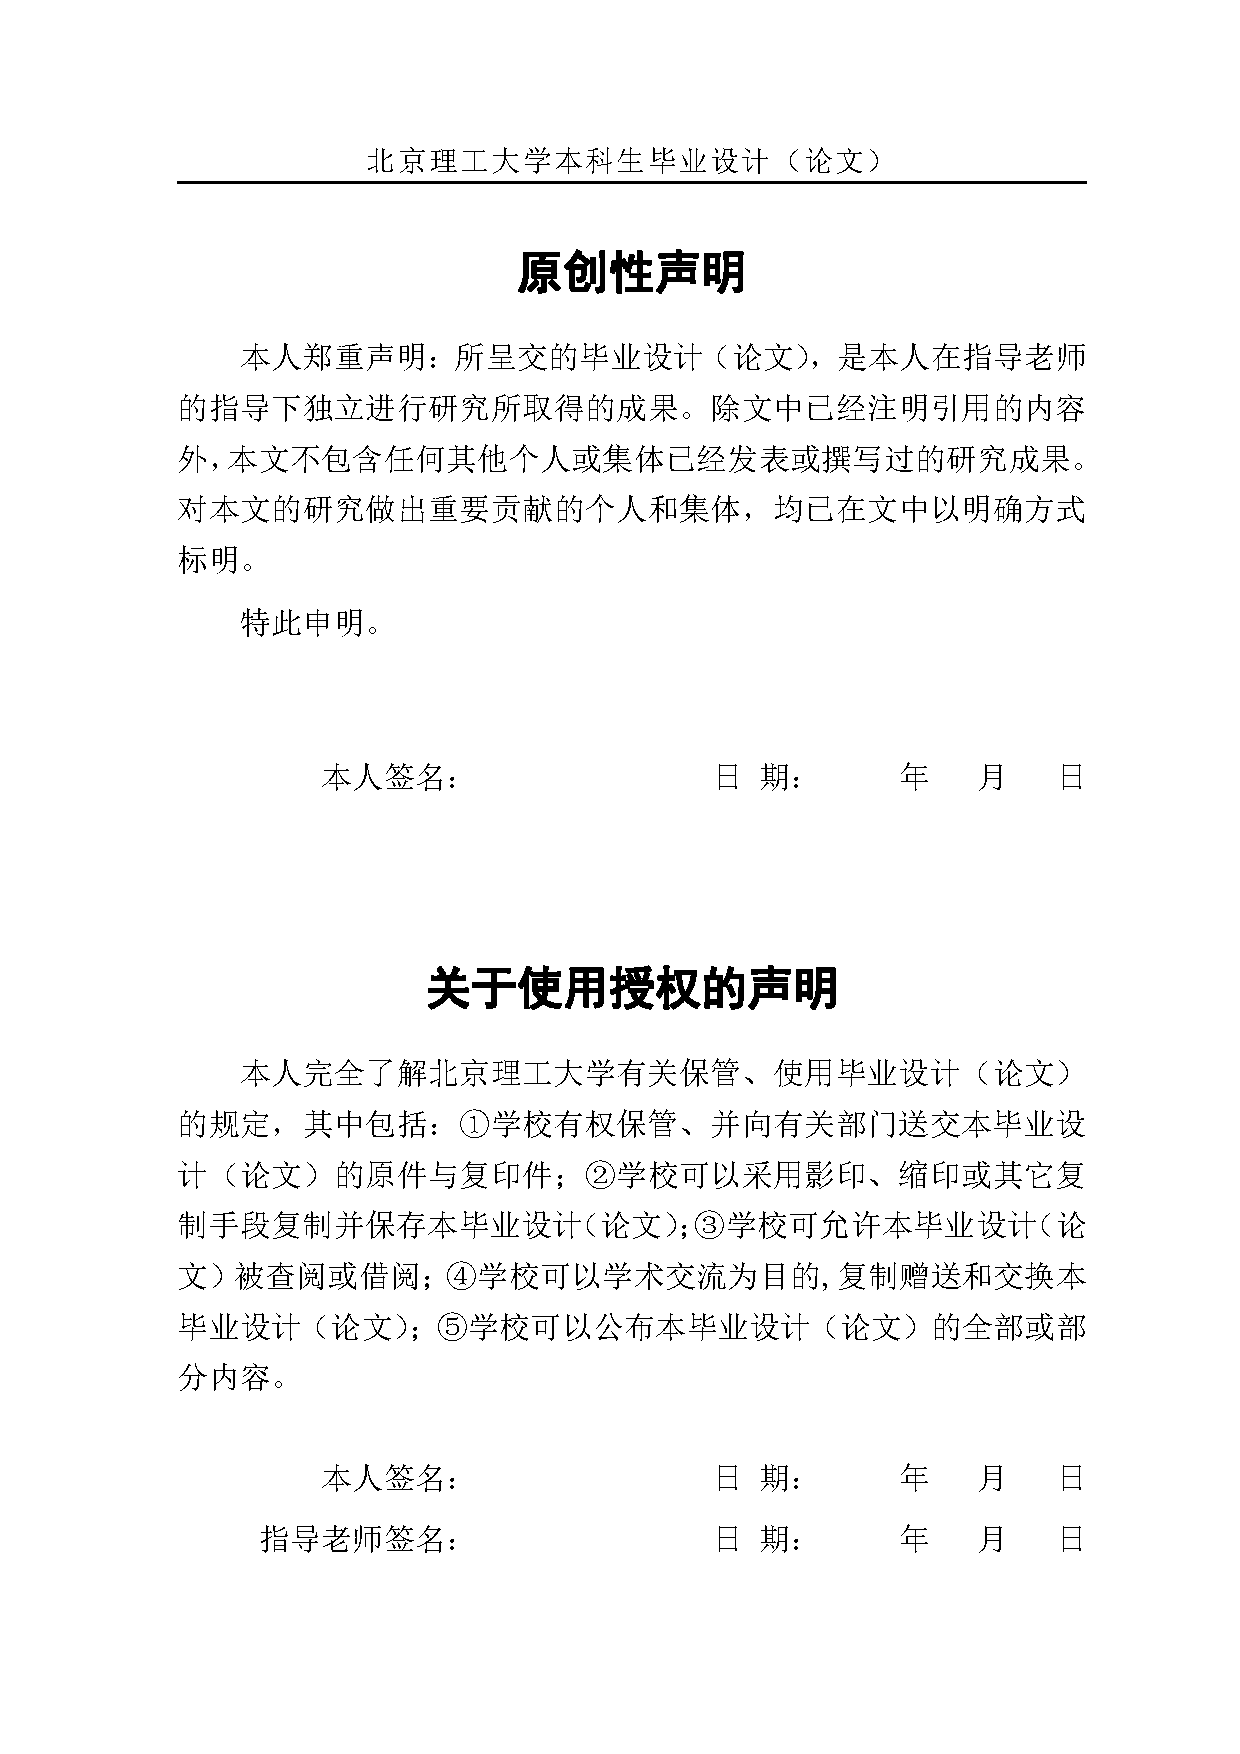
\includepdf{misc/1_originality.pdf}\newpage
\end{blindPeerReview}
% ====== 原创性声明(PDF 格式)======
% ====== 原创性声明(LaTeX 格式)======
% %%
% The BIThesis Template for Bachelor Graduation Thesis
%
% 北京理工大学毕业设计(论文)原创性声明模板 —— 使用 XeLaTeX 编译
%
% Copyright 2020-2023 BITNP
%
% This work may be distributed and/or modified under the
% conditions of the LaTeX Project Public License, either version 1.3
% of this license or (at your option) any later version.
% The latest version of this license is in
%   http://www.latex-project.org/lppl.txt
% and version 1.3 or later is part of all distributions of LaTeX
% version 2005/12/01 or later.
%
% This work has the LPPL maintenance status `maintained'.
%
% The Current Maintainer of this work is Feng Kaiyu.
%
% Compile with: xelatex -> biber -> xelatex -> xelatex
%
% 如无特殊需要,本页面无需更改

\MakeOriginality

% ====== 原创性声明(LaTeX 格式)======

% 前置页面定义
\frontmatter
% 摘要:在摘要相应的 TeX 文件处进行摘要部分的撰写
%%==================================================
%% abstract.tex for BIT Master Thesis
%% modified by yang yating
%% version: 0.1
%% last update: Dec 25th, 2016
%%==================================================
\begin{abstractEn}
    In the contemporary era of rapid technological advances and escalating trade protectionism, this thesis investigates the environmental implications of trade policies with a focus on the semiconductor industry. This research is crucial as it bridges the gap between global trade dynamics and environmental sustainability, highlighting the pressing need to understand and mitigate the environmental consequences of international commerce.

    This study employs a multi-regional input-output (MRIO) model to delve into the environmental impacts of trade, specifically analyzing how no-trade scenarios and a novel approach to global production share redistribution (GPSR, also refered as gaming scenario) influence carbon emissions between major trading nations like the United States and China. The focus on the semiconductor industry provides a detailed lens through which to assess both upstream and downstream effects on carbon footprints under various hypothetical trade restrictions. The methodology not only quantifies the direct impacts of trade but also explores sophisticated redistributive scenarios that reflect contemporary global trade complexities.

    The findings reveal that the current Sino-US trade relationship, particularly under the GPSR scenario, significantly mitigates global carbon emissions, with a documented carbon reduction of 0.3568\% globally for semiconductor related products. This contradicts common perceptions that trade protectionism inherently benefits environmental outcomes. Instead, the study demonstrates that strategic trade engagements and redistribution of production responsibilities can effectively reveal the carbon uplift under no trade scenario.

    Based on these insights, the thesis proposes robust policy recommendations aimed at fostering sustainable trade practices. These include enhancing international cooperation, integrating environmental standards into trade agreements, promoting technology transfers, and establishing comprehensive global emissions monitoring frameworks. Such policies are essential for leveraging trade as a tool for environmental improvement, ensuring that economic development does not come at the cost of ecological degradation.

    This research significantly contributes to academic discussions on trade and environment, offering policymakers and industry stakeholders valuable strategies to align economic activities with environmental conservation, thereby supporting a balanced approach to global trade and sustainability.

\end{abstractEn}

\begin{abstract}
    在快速技术进步和日益加剧的贸易保护主义的当今时代,本文研究了贸易政策对环境的影响,重点聚集于半导体行业。这项研究至关重要,因为它弥合了全球贸易动态与环境可持续性之间的差距,突显了理解和减轻国际商业环境后果的迫切需要。

本研究采用多区域投入产出(MRIO)模型深入探讨贸易的环境影响,特别是分析无贸易情景和全球生产份额重新分配(GPSR,也被后文指代为基于博弈分配的方法)这一新方法如何影响美国和中国等主要贸易国之间的碳排放。聚焦半导体行业提供了一个细致的视角,用以评估各种假设贸易限制下的上游和下游对碳足迹的影响。该方法不仅量化了贸易的直接影响,还探讨了反映当代全球贸易复杂性的复杂重新分配情景。

研究结果显示,当前中美贸易关系,特别是在GPSR情景假设下,显著减少了全球碳排放(半导体相关产品的全球碳减少量为0.3568\%)。这与普遍认为的贸易保护主义固有地有利于环境结果的看法相矛盾。相反,本研究表明,战略贸易参与和生产责任的重新分配可以有效地揭示无贸易情景下的碳上升。

基于这些洞见,论文提出了旨在促进可持续贸易实践的强有力政策建议。这些包括加强国际合作、将环境标准整合到贸易协议中、推广技术转移以及建立全面的全球碳排放监测框架。这些政策对于将贸易作为环境改善工具至关重要,确保经济发展不以生态退化为代价。

本研究对贸易与环境的学术讨论作出了重大贡献,为政策制定者和行业利益相关者提供了将经济活动与环境保护兼顾的宝贵策略,从而支持全球贸易和可持续性的平衡发展。
   

\end{abstract}
   


\MakeTOC

% 正文开始
\mainmatter

% 第一章

%%==================================================
%% chapter01.tex for BIT Master Thesis
%% modified by yang yating
%% version: 0.1
%% last update: Dec 25th, 2016
%%==================================================
\chapter{Introduction}
\label{chap:INTRODUCTION}
\section{Reseach Background}
The interplay between global commerce and environmental sustainability has escalated into a prominent area of scholarly investigation, reflecting the growing complexity of international trade's impact on ecological systems (\supercitet{RN123}; \supercitet{RN166}). In the wake of increasing global interconnectedness, 2022 saw international trade account for more than 30\% of global GDP, while also contributing significantly to global carbon emissions—exceeding one-quarter of the total emissions (\supercitet{RN176}). This significant environmental footprint underscores the urgent need to explore the mechanisms through which global trade practices distribute pollutants across regions, particularly highlighting stark disparities in pollution levels between developed and developing nations (\supercitet{RN133}; \supercitet{RN161}).

Historically, the relocation of pollution-intensive industries from developed to less regulated developing regions has been perceived as a strategic move to circumvent stringent environmental laws, thereby raising critical questions about the actual environmental cost of free trade. This shift not only exacerbates the emission levels in developing regions but also complicates the global efforts to mitigate environmental impacts (\supercitet{RN169}). The global trade environment is further complicated by recent geopolitical events, including intensifying trade frictions between major economies such as the U.S. and China, Brexit implications, the establishment of regional trade barriers (\supercitet{RN160}), and significant policy enactments like the U.S. export controls. The onset of the 2020 pandemic added another layer of complexity, propelling nations towards an unprecedented level of protectionism characterized by severe trade restrictions (\supercitet{RN143}; \supercitet{RN111}).

Focusing on the U.S.-China trade dynamics as detailed in Table \ref{tab:timeline}, this research seeks to dissect the environmental outcomes of these economic interactions. As the two largest global economies and leading carbon emitters, the trade activities between these nations not only shape economic landscapes but also significantly influence global environmental policies and practices. In 2019, the U.S. and China accounted for 28\% and 14\% of global CO2 emissions respectively, with their bilateral trade constituting a significant portion of the world trade (\supercitet{RN180}). The recent trade disputes, marked by the U.S.'s CHIPS and Science Act and China's strategic export controls, offer a compelling case study to explore the environmental ramifications of these economic engagements.

The semiconductor industry occupies a unique position within the U.S.-China trade landscape, characterized by its high technological intensity and strategic significance. This sector not only drives significant economic value but also acts as a focal point in the technological rivalry between these two global powers. The intricacies of semiconductor trade between the U.S. and China are highlighted by the frequent shifts in policy, ranging from the U.S. imposing restrictions on semiconductor exports to China, to China's maneuvers to bolster its domestic chip manufacturing capabilities in response (\supercitet{RN180}). These dynamics are critical as they not only influence trade policies but also affect global supply chains and innovation trajectories in technology-intensive sectors.

The environmental impacts of this trade are multifaceted. On one hand, the advanced technologies used in semiconductor manufacturing require substantial resources, including water and energy, and involve the use of hazardous chemicals, which pose significant environmental risks if not managed properly (\supercitet{RN176}). On the other hand, the drive towards more advanced semiconductor technologies can lead to more energy-efficient products, potentially mitigating some of the environmental impacts associated with electronic devices' life cycles. However, the escalation of trade tensions and the resulting shifts in production locations may lead to environmental deregulation as countries compete for manufacturing dominance. This scenario can exacerbate the environmental costs in regions that may adopt less stringent environmental controls to attract or retain semiconductor manufacturing facilities. Thus, understanding the environmental outcomes of semiconductor trade requires a nuanced approach, considering both the direct impacts of manufacturing and the broader implications of global trade policies on environmental standards and practices.

This enriched backdrop serves as the foundation for this study, aiming to provide an in-depth analysis of how shifts in global trade policies, particularly those influenced by major geopolitical events, affect environmental outcomes. Through this lens, the research will examine the broader implications of international trade on global sustainability efforts, making it crucial to understand and possibly reframe the ongoing discourse on trade and environment in the contemporary global economy.

\begin{table}
     \centering
     \caption{U.S. and China Relationship in the context of trade tension timeline} \label{tab:timeline}
     \begin{tabular}{|p{0.1\textwidth}|p{0.9\textwidth}|}
     \toprule
       Year & Event \\
     \midrule
       2000 & Normalization of trade relations between the U.S. and China. \\
       2008 & China becomes the largest U.S. foreign creditor. \\
       2010 & China becomes the world's second-largest economy. \\
       2011 & U.S. 'pivots' toward Asia, countering China's growing clout, and announces the Trans-Pacific Partnership. \\
       2012 & Rising U.S.-China trade tensions, with the U.S. trade deficit with China reaching an all-time high of \$295.5 billion. \\
       2013 & Sunnylands Summit between U.S. and China leaders. \\
       2016 & China aims to reduce energy intensity by 15\% under its 13th Five-Year Plan. \\
       2017 & China commits to investing \$360 billion in renewable energy by 2020, reducing coal reliance. \\
       2018 & The U.S. imposes tariffs on Chinese goods, marking the beginning of the U.S.-China trade war. \\
       2020 & China leads in renewable energy, investing in solar panels and wind turbines. \\
            & The 'Phase One' trade deal is signed amid rising tensions due to the COVID-19 pandemic. \\
            & The U.S. imposes restrictions on China's semiconductor industry. \\
            & Huawei faces severe U.S. restrictions, leading to a substantial revenue decline. \\
            & China already has \$150 billion in chip subsidies. \\
       2021 & Biden administration enhances restrictions on China's semiconductor industry. \\
       2022 & The U.S. Congress passes the CHIPS and Science Act, providing subsidies and tax breaks to boost domestic semiconductor production. \\
            & Additional sanctions are imposed on Chinese companies, and the entity list of restricted companies expands significantly. \\
            & The National Defense Authorization Act prohibits U.S. government agencies from procuring products containing semiconductors made by China's leading chip manufacturers. \\
            & Huawei's partner, SMIC, achieves a breakthrough in 7nm chip manufacturing. \\
            & Japan announces restrictions on exporting 23 types of equipment used in chip-making processes to China. \\
            & President Xi Jinping announces the New Whole Nation System for self-reliance in critical national security technologies. \\
       2023 & China introduces a new export license system for gallium and germanium. \\
            & The Netherlands limits exports to China of deep ultraviolet lithography machines. \\
            & U.S. restricts export of cutting-edge chips and chip-making equipment to China. \\
            & The U.S. implements the Advanced Computing Chips Rule and the Expansion of Export Controls on Semiconductor Manufacturing Items Interim Final Rule. \\
            & Introduction of two new Temporary General Licenses (TGLs). \\
            & Huawei launches Mate 60 and Mate 60 Pro with HiSilicon Kirin 9000S processors. \\
            & U.S. Commerce Department finalizes guardrails limiting expansion in China for companies receiving subsidies under the 2022 CHIPS and Science Act. \\
            & China upgrades its semiconductor R\&D tax credit by 20\%. \\
   \bottomrule
   \end{tabular}
   \end{table}
   
\section{Research Content}

This study delves into the intricate dynamics of trade protectionism and its environmental repercussions, particularly focusing on the semiconductor industry and its significant role within the broader framework of global trade and carbon emissions. Utilizing the extensive dataset from Exiobase3 covering the period from 2000 to 2022, the research adopts a nuanced methodological approach that goes beyond traditional binary analyses of trade scenarios. Instead, it explores a graduated range of trade restriction scenarios to provide a more detailed understanding of their environmental impacts.

The research is structured around several key investigative areas. Initially, the study quantifies the carbon emissions linked to the semiconductor trade, employing the MRIO model to map out the flow of goods and associated emissions across international boundaries. This step is crucial in understanding the primary sources of emissions and the extent to which trade can influence global carbon footprints. By comparing actual trade scenarios with hypothetical no-trade conditions, the research highlights the significant role trade policies play in shaping environmental outcomes.

Moreover, the research employs a sophisticated cooperative game theoretical framework to analyze the complex effects of trade protectionism across different nations. This approach allows for an in-depth exploration of how trade policies influence global CO2 emissions, bridging the gap between economic activities and environmental outcomes. The game-theoretical model facilitates an understanding of the strategic interactions among nations, considering both competitive and cooperative behaviors in the global trade arena.

The primary objective of this research is to provide a profound comprehension of the complex interplay between trade policies and environmental sustainability. It seeks to uncover the nuanced implications of trade protectionism, particularly in technologically advanced sectors, against the backdrop of ongoing trade conflicts between the United States and China. The study aims to offer insights into how current and future trade policies might shape global environmental sustainability, especially in terms of carbon emissions, within the increasingly globalized economic landscape.

By advancing these methodological innovations and analytical frameworks, the research contributes significantly to the academic discourse on trade and environment. It provides policymakers and scholars with a deeper understanding of how trade dynamics influence environmental outcomes, emphasizing the need for integrated approaches to managing trade and environmental policies in a way that supports sustainable global development.

\section{Research Significance}
The significance of this research extends across both theoretical and practical dimensions, contributing profoundly to the discourse on trade, technology, and environmental sustainability. Theoretically, this study enhances the application of multi-regional input-output (MRIO) models and cooperative game theoretical frameworks within the context of international trade and environmental impacts. By integrating these sophisticated methodologies, the research enriches the analytical approaches available for examining the environmental consequences of trade policies. This theoretical advancement not only broadens the scope of economic models in environmental studies but also introduces a nuanced perspective on the interplay between trade dynamics and global sustainability efforts.

From a practical standpoint, the findings of this research hold substantial implications for policymakers and industry stakeholders. By demonstrating the environmental benefits of current trade structures, particularly within the semiconductor industry, the study provides essential insights that can inform policy decisions. The detailed analysis of carbon emission shifts under various trade scenarios offers a valuable tool for governments and international organizations to assess the potential outcomes of trade policies on environmental sustainability. This is particularly pertinent in the context of ongoing global discussions about trade agreements and environmental regulations.

Furthermore, the insights derived from this research regarding the semiconductor industry's role in global carbon emissions are critically important for industry stakeholders. As semiconductor manufacturing is both energy-intensive and central to modern technology, understanding its impact on carbon emissions is crucial for developing more sustainable production practices. The data-driven insights provided by this study could guide the semiconductor industry in adopting greener technologies and practices that align with global carbon reduction goals.

In summary, the research not only contributes to academic knowledge by applying and expanding upon advanced methodological frameworks but also serves as a strategic guide for policymakers and industry leaders. By elucidating the complex relationship between trade policies and environmental outcomes, it supports informed decision-making that could lead to more effective environmental strategies and trade agreements. This dual contribution underscores the relevance and urgency of integrating economic and environmental considerations in the planning and implementation of trade policies worldwide.


\section{Thesis Structure}

This thesis is meticulously organized into five chapters, each delineating a distinct aspect of the study, designed to provide a comprehensive understanding of the interplay between trade policies and environmental impacts, with a specific focus on the semiconductor industry.

\textbf{Chapter 1 Introduction} sets the stage for the research by presenting the background, which articulates the relevance of exploring the environmental implications of global trade, particularly within the context of rising trade protectionism and technological advancements in semiconductor production. The research content, significance, and a detailed structure of the thesis are also outlined, providing a clear roadmap for the reader.

\textbf{Chapter 2 Literature Review} explores existing scholarly work related to the environmental consequences of international trade, with an emphasis on input-output analysis. This chapter is divided into four sections, each reviewing different aspects of the literature that discuss environmental impacts from trade, the dual outcomes of trade frictions, specific issues concerning the semiconductor industry, and new paradigms in assessing the impact of global production-based redistribution. This comprehensive review helps to position the current study within the existing body of knowledge and identifies gaps that the research aims to fill.

\textbf{Chapter 3 Methodology and Data} describes the analytical frameworks and data sources used in this study. It begins with a detailed explanation of the MRIO model employed to calculate trade-related variables and assess carbon footprints. The chapter progresses to discuss the unique scenarios modeled in this study, including no-trade conditions, and concludes with the methodologies used for data collection, primarily focusing on the use of Exiobase3. This methodological groundwork is essential for understanding the subsequent analysis of trade impacts on global carbon emissions.

\textbf{Chapter 4 Empirical Results} presents the findings from the application of the methodologies described in Chapter 3. This chapter is structured to sequentially address the research questions posed, analyzing the global carbon emissions related to international trade, the differences between production-based and consumption-based accounting of emissions, and the specific impacts of semiconductor trade under various hypothetical trade scenarios. Detailed analysis of the semiconductor industry's upstream and downstream impacts on global carbon emissions is also provided. This chapter is crucial as it translates the theoretical and methodological frameworks into practical insights.

\textbf{Chapter 5 Conclusions and Policy Recommendations} synthesizes the findings from the empirical analysis, highlighting the nuanced implications of trade protectionism on carbon emissions globally. The chapter offers concrete policy recommendations based on the research findings, aimed at optimizing trade practices to enhance global environmental outcomes. It also reflects on the broader implications of these findings for policymakers, industry stakeholders, and the academic community.

Throughout the thesis, references and appendices provide additional support and resources, including detailed descriptions of semiconductivity-related products and a list of ISO 3166-1 country codes, which assist in understanding the technical aspects and geographical scope of the research. This structured approach ensures a logical flow of information, facilitating a thorough understanding of the complex relationships between trade and environmental sustainability.

\ifincludefigures
\begin{figure}
\centering
\makebox[\textwidth][c]{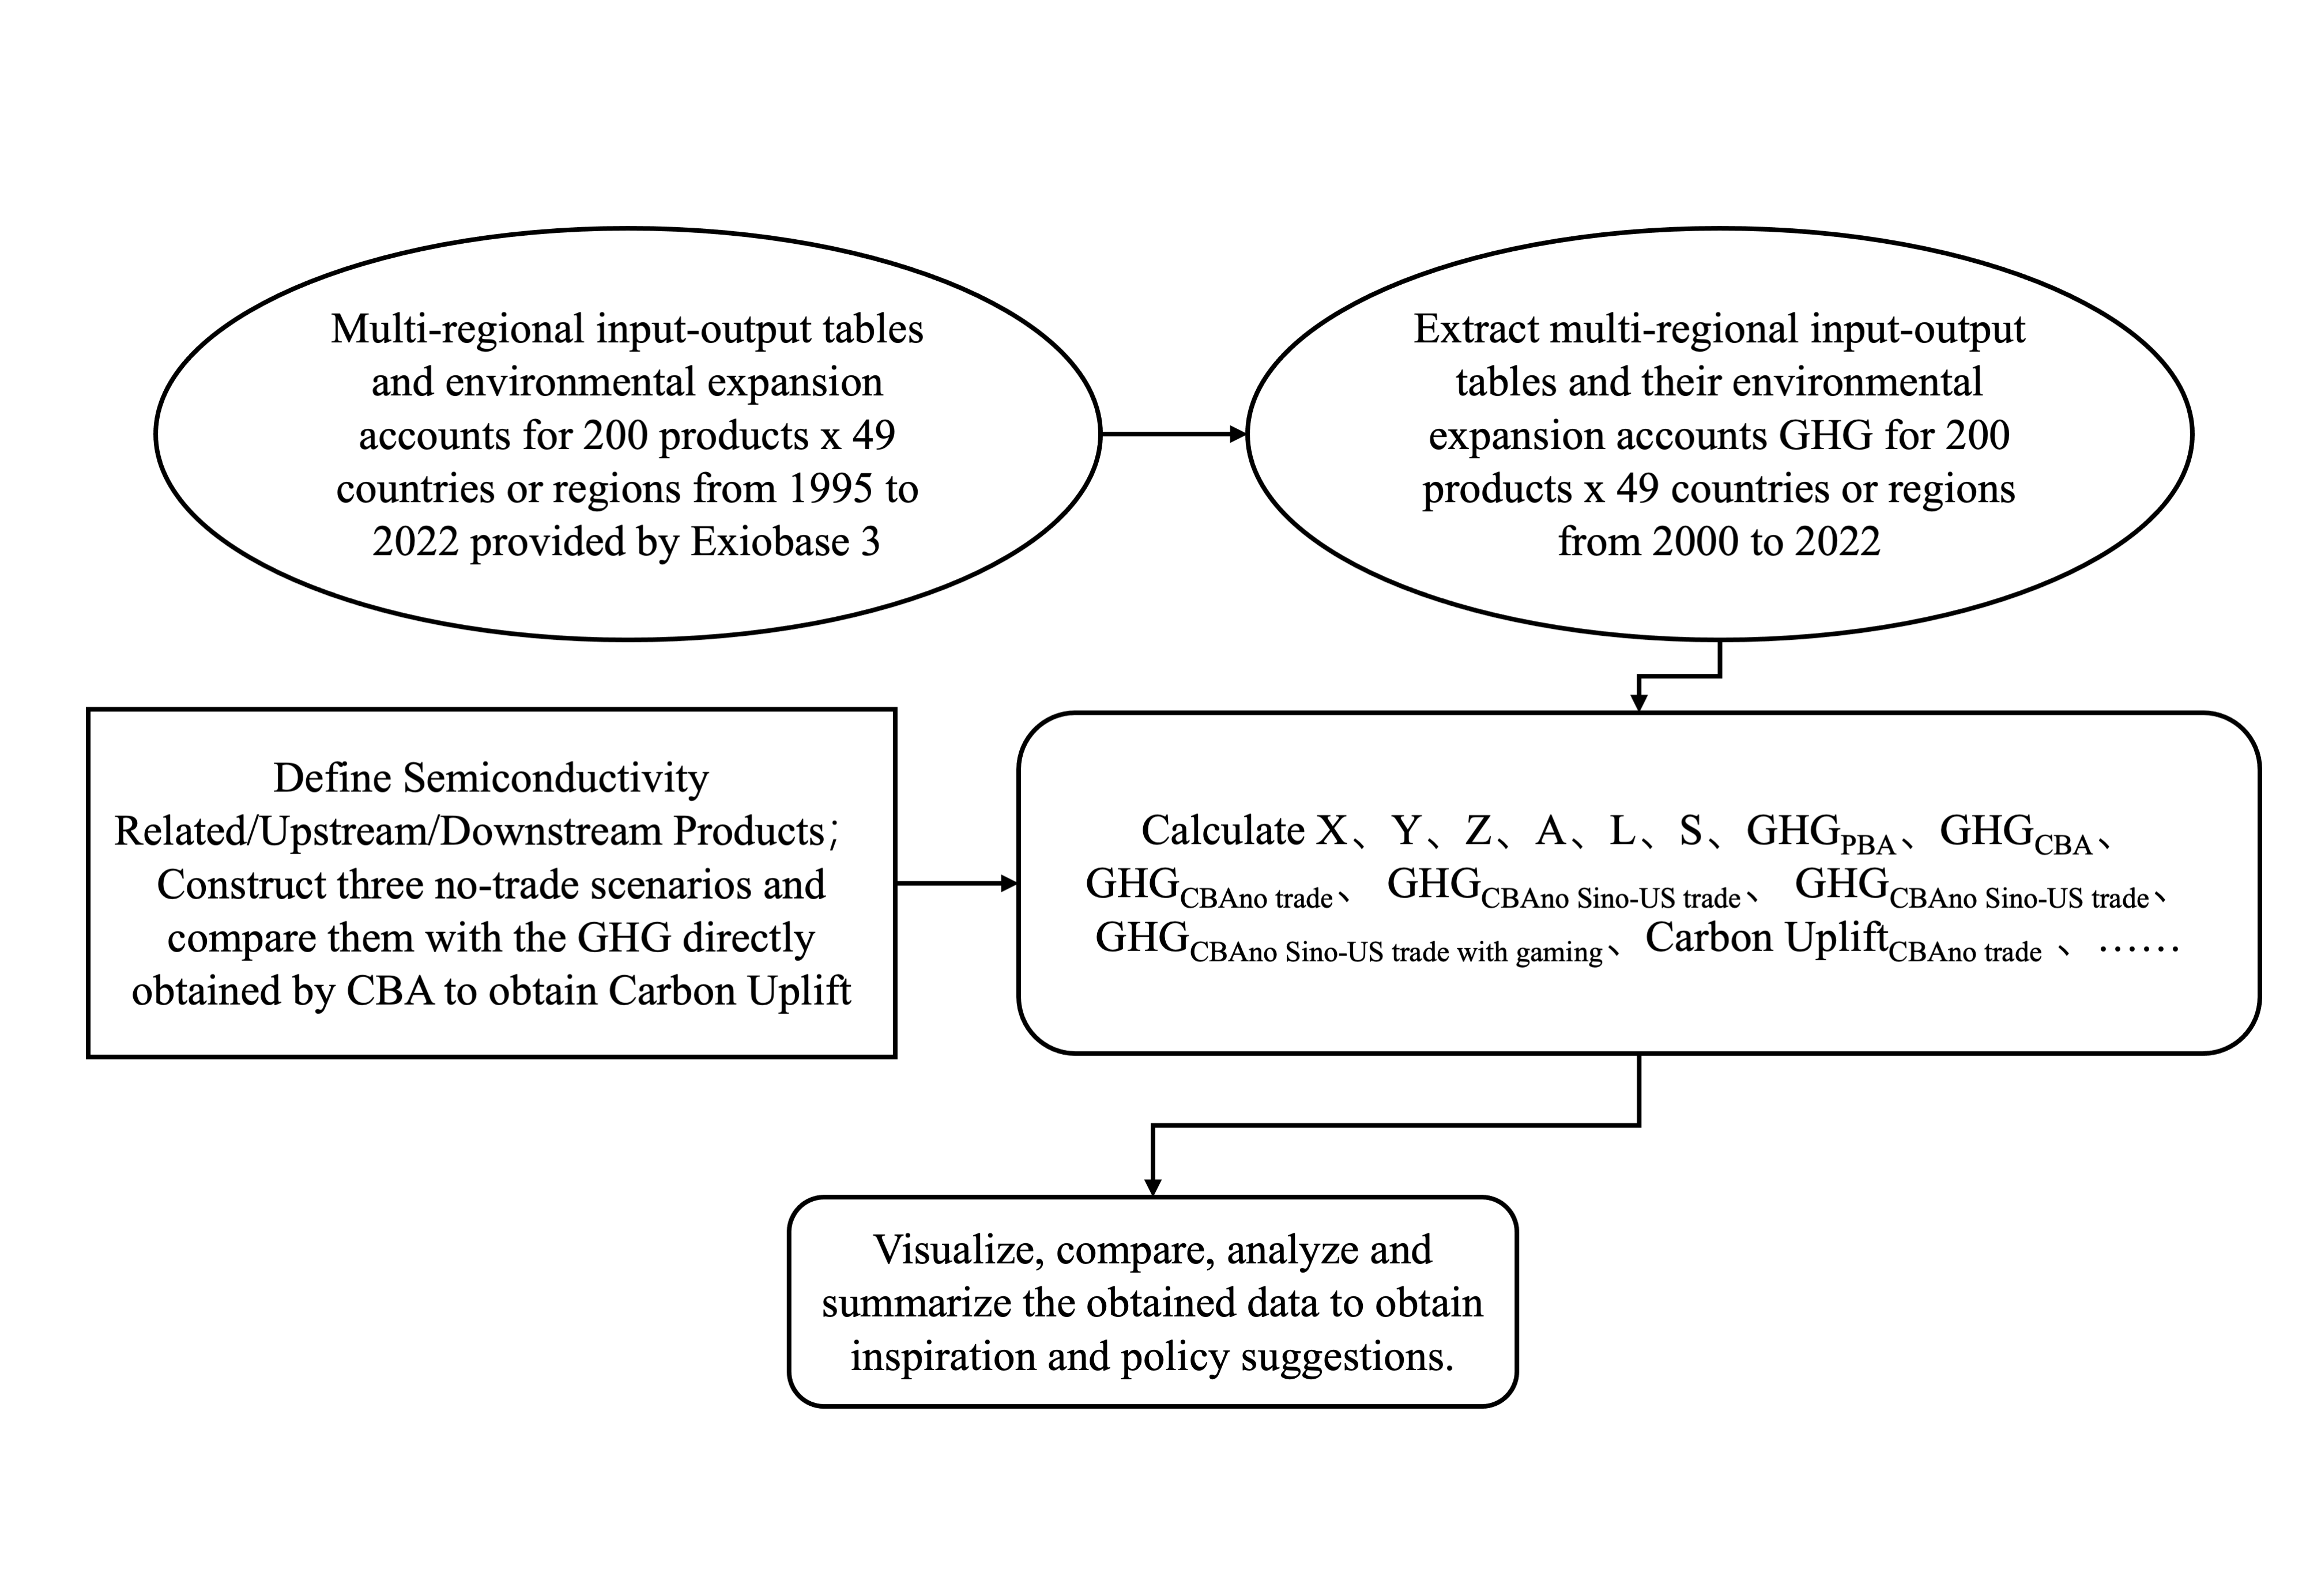
\includegraphics[width=1\textwidth]{figures/Graph/幻灯片2.png}}
 \caption{Technical Roadmap}\label{fig:tech roadmap}
\end{figure}
\fi                                                                                                                                                                                     
Figure \ref{fig:tech roadmap} illustrates the structured methodology employed in this thesis to analyze the environmental impacts of international trade, with a specific focus on the semiconductor industry, utilizing multi-regional input-output (MRIO) tables and environmental expansion accounts provided by Exiobase 3. The approach is divided into several key stages to ensure a comprehensive assessment of the trade-related carbon footprint.

Initially, the study extracts MRIO tables and their corresponding environmental data covering the years 2000 to 2022 for 200 products across 49 countries or regions. This extensive data extraction forms the basis for all subsequent analyses, offering a detailed and expansive perspective on global trade and environmental interactions.

Following data extraction, the study defines specific product categories related to semiconductivity, including upstream and downstream products. These categories are crucial for focusing the analysis on relevant sectors within the semiconductor industry. The research constructs three distinct no-trade scenarios to simulate the environmental impacts in the absence of trade. These scenarios are compared with actual greenhouse gas emissions data obtained through consumption-based accounting (CBA), allowing for a nuanced calculation of carbon uplift due to trade activities.

The core analytical phase involves calculating various elements such as total output ($X$), intermediate inputs ($Z$), final demand ($Y$), and the Leontief inverse matrix ($L$), which are foundational to understanding the economic interconnections within the MRIO framework. These calculations lead to the estimation of greenhouse gas emissions under different trade scenarios, including no-trade, no Sino-US trade, and a scenario incorporating gaming trade redistribution, which offers insights into potential changes in carbon emissions patterns due to strategic alterations in trade policies.

The final stage of the methodology involves a detailed visualization, comparison, and analysis of the data to draw meaningful conclusions and generate policy recommendations. This process not only elucidates the quantitative impacts of trade on carbon emissions but also provides a solid empirical foundation for suggesting strategic interventions to optimize trade practices for better environmental outcomes.

The technical roadmap, as visualized in Figure \ref{fig:tech roadmap}, is integral to demonstrating the systematic approach taken in this thesis to address the complex interplay between trade and environmental policies. This structured methodology ensures that the findings are robust, comprehensive, and relevant to policymakers and industry stakeholders engaged in navigating the challenges of sustainable international trade.
%%==================================================
%% chapter01.tex for BIT Master Thesis
%% modified by yang yating
%% version: 0.1
%% last update: Dec 25th, 2016
%%==================================================
\chapter{Literature Review}
\label{chap:LITERATURE REVIEW}

\section{Environmental Consequences of Trade: Insights from Input-Output Analysis}
The environmental ramifications of global commerce have been meticulously scrutinized through the lens of input-output analysis, which has become a pivotal instrument for unraveling the complex relationship between economic activities and environmental impacts. Dating back to the 1970s, this methodology has provided significant insights (\supercitet{RN119}). In contemporary research, the scope of input-output analysis has broadened to include comprehensive assessments of environmental and societal repercussions within the entire span of global supply chains (\supercitet{RN158}; \supercitet{RN167}; \supercitet{RN171}; \supercitet{RN154}; \supercitet{RN172}). Pivotal examinations of global multi-regional input-output (GMRIO) databases, such as the ones articulated by \supercitet{RN170}, have been central to tracing the intricate connections linking nascent production zones to regions with high levels of consumption, shedding light on the extensive environmental and societal effects of international commerce. The progressive engagement of emerging economies in the global marketplace has precipitated an intensified migration of pollutive emissions to these locales, reaffirming the view that global trade amplifies environmental burdens in the developing world (\supercitet{RN127}; \supercitet{RN164}). Although there exists a temporal gap in the refreshment of input-output tables, sometimes extending to as late as 2014, these datasets remain crucial in characterizing socio-economic constructs and continue to hold significance for studies on trade. This scholarly landscape sets the stage for this investigation, which aims to delve deeper into the environmental outcomes of global trade, particularly under the influence of the recent shifts in the global economic climate.

\section{Trade Frictions and Environmental Outcomes: A Dualistic Evaluation}
Trade disputes are characterized by a multifaceted environmental impact, with both favorable and adverse consequences. On one flank, academic discourses, such as the one by \supercitet{RN141}, argue that trade constraints might lead to a tangible reduction in global carbon dioxide emissions by scaling back industrial operations and advocating for regional self-sustenance. Empirical evidence suggests that increased trade friction can mitigate greenhouse gas emissions, alter the global distribution of these emissions, and potentially enhance air quality across numerous countries. It postulates that continued governmental imposition of tariffs could precipitate a contraction in global greenhouse gas emissions, possibly up to 5\% (\supercitet{RN142}). Conversely, there are detrimental impacts to consider. Literature such as \supercitet{RN132} warns that while the dissolution of trade barriers can catalyze economic advancement and the adoption of greener technologies, the establishment of such barriers could obstruct these positive trends. In addition, the work of \supercitet{RN147} alongside \supercitet{RN142} emphasizes that trade disagreements, notably the trade conflict between China and the US, may instigate a surge in emissions in regions that shift to manufacturing hubs with more lenient environmental standards. These conflicting insights highlight the complexity inherent in the environmental effects of trade policies, underscoring the need for a holistic viewpoint to comprehend the intricate dynamic between trade tensions and global environmental health.

\section{Semiconductor Trade and Environmental Dynamics: A Critical Inquiry}
In the endeavor to contextualize the semiconductor industry within the broader framework of global trade and its environmental implications, one encounters a notable scarcity of comprehensive studies that intersect these three elements. Among the sparse literature that does delve into these intersections, the article by Mullen and Morris (2021)\cite{WOS:000657017300001} emerges as a crucial reference. They examine the ecological repercussions of semiconductor chip manufacturing from a life cycle perspective, emphasizing the pivotal role that nanofabrication technologies might play in enhancing sustainability within the sector .

Despite its insightful contributions, Mullen and Morris's study stands relatively alone in the academic landscape. It articulates concerns about the toxicological impacts associated with the vast quantities of solvents, acids, and gases used in chip production. Furthermore, it highlights the potential of directed self-assembly of block copolymers as a sustainable alternative to traditional lithographic processes. This perspective is invaluable, as it not only underscores the environmental challenges but also proposes innovative solutions within the semiconductor manufacturing process.

However, the current body of literature, lacking extensive examination of the interplay between semiconductor trade, environmental issues, and international commerce, does not reflect the complex dynamics illustrated in recent trade disputes, particularly those involving the United States and China. These disputes frequently revolve around the semiconductor industry, as detailed in Table \ref{tab:timeline}. For instance, legislative actions such as the U.S. CHIPS and Science Act of 2022, along with various sanctions and export restrictions, underscore the strategic importance and contentious nature of this sector in global trade relations.

This study aims to fill the noted gap by providing a thorough analysis of how semiconductor trade impacts environmental outcomes on a global scale, informed by these recent geopolitical developments. The unique and critical position of semiconductors in modern technology and international security, coupled with the environmental considerations highlighted by Mullen and Morris, justify a deeper exploration into this field. It is hoped that this research will catalyze further academic inquiry into the nuanced relationships between trade, technology, and the environment, particularly in sectors as pivotal as semiconductors.

\section{Global Production-Based Redistribution: A New Paradigm in Trade Impact Analysis}
Recent analyses of global trade dynamics have underscored the dual role of international commerce as both a vehicle for economic expansion and a catalyst for environmental change. A significant body of work (\supercitet{does_protectionism_improve_environment}; \supercitet{production_fragmentation_and_inter-provincial_trade_water_china}; \supercitet{China's_inter-provincial_trade}) has depicted the intricate relationship between the liberalization of trade and its environmental repercussions, particularly emphasizing the augmented burden of pollution borne by developing economies as a consequence of 'pollution outsourcing' by their developed counterparts. The advent of protectionist policies, resurging notably in the wake of the COVID-19 pandemic, presents an opportune research nexus to evaluate the environmental ramifications of such trade barriers.

Protectionism, though conventionally understood as an impediment to economic interdependence, introduces an intriguing dimension to environmental efficiency. The prevailing discourse (\supercitet{does_protectionism_improve_environment}) evaluates this through the lens of multi-regional input-output (MRIO) models and data envelopment analysis (DEA), presenting a dichotomy: while territorial emissions may wane under protectionist regimes, environmental efficiency does not necessarily parallel this decline. This divergence propels the discourse towards a more nuanced understanding of trade's environmental impact.

Inter-provincial analyses (\supercitet{production_fragmentation_and_inter-provincial_trade_water_china}) further delineate the multifaceted effects of trade, where production fragmentation and trade patterns reveal disparate impacts on regional water scarcity. It becomes evident that trade's influence extends beyond mere economic transfers, encompassing complex virtual water networks that underpin trade relationships.

In the context of China, trade has played a dichotomous role in advancing and inhibiting Sustainable Development Goals (SDGs), with inter-provincial trade being particularly pivotal (\supercitet{China's_inter-provincial_trade}). The examination of these SDG indicators through MRIO models over time furnishes insights into the spatial dynamics of trade's influence, demonstrating the heterogeneity of impacts across different provinces and timeframes.

The discourse then pivots to the quantified impacts of international trade on carbon intensity, where studies (\supercitet{impacts_of_US_carbon_intensity}) highlight the United States' progression towards emission reduction, facilitated to an extent by the transference of emissions through international trade. Such findings pivotally inform the current study, which innovates upon this dialogue by integrating a nascent perspective — the potential allocation of trade gaps based on a Nash equilibrium-inspired approach within the MRIO framework.

This study posits a groundbreaking methodology to estimate the repercussions of partial trade protectionism, specifically between China and the United States, on the semiconductor industry's global carbon footprint. Rejecting the oversimplified assumption of total domestic production replacement in the wake of trade cessation, this research proposes a redistribution mechanism predicated on the proportional global production shares detailed in the MRIO tables. This approach, enlightened by Nash equilibrium concepts, suggests that the competitive interplay following a trade gap would mirror pre-existing production and trade structures. Such an approach has not been previously explored in the literature, thereby charting a new trajectory for future research.

In essence, this literature review situates the current study at the vanguard of trade and environmental research. By transcending the conventional binaries of trade versus protectionism, it endeavors to capture the complexities of a globalized economy's adaptive mechanisms in the face of shifting trade policies.

\chapter{Methodology and Data}
\label{chap:METHODOLOGY AND DATA}

\section{Trade-Related Variables Calculation: MRIO Model}

The input-output model is a powerful tool for analyzing the environmental impacts of human economic activities within a complex system. It details the quantitative dependencies between production and consumption and sheds light on both the direct and indirect economic connections across global sectors (\supercitet{RN135}). This model has evolved from assessing single regions to more intricate multi-regional input-output analyses (MRIO), which precisely identify the sources of imports (\supercitet{RN145}). Furthermore, the incorporation of environmental metrics into the MRIO model allows for a detailed examination of the relationships between economic activities and their environmental impacts, making it a widely used tool to track the environmental footprints of global trade.

Adhering to traditional production theory, trade involves the consumption of various resources and services to produce economic outputs (\supercitet{RN128}). In this study, we conceptualize the environmental production framework concerning trade, identifying capital, labor, and energy as inputs; value added as the desirable output; and pollutants as the undesirable outputs. We focus on greenhouse gases—major contributors to global warming and atmospheric pollutants like acid rain and photochemical smog—as primary indicators of environmental impact (\supercitet{RN125}; \supercitet{RN150}; \supercitet{RN175}).

Utilizing the MRIO model, we establish a list of trade-related variables under scenarios of actual trade and hypothetical no-trade conditions. The differential in emissions of the three selected pollutants under these scenarios highlights the direct environmental impact of trade protection measures. Assume the global economy consists of N interconnected economies, each comprising S specific industrial sectors:

\begin{align}
X_1 &= Z_{11} + Z_{12} + \cdots + Z_{1N} + Y_1 \notag \\
X_2 &= Z_{21} + Z_{22} + \cdots + Z_{2N} + Y_2 \notag \\
&\ \vdots \notag \\
X_N &= Z_{N1} + Z_{N2} + \cdots + Z_{NN} + Y_N
\label{eq:X_Z}
\end{align}
where Xi, Yi, Zij denote the total output matrix (S x 1) of economy i, the final demand matrix (S x 1) for economy i, and the intermediate inputs matrix from economy i to economy j (S x S), respectively. These matrices are economic variables expressed in monetary units, typically dollars.
The technical coefficient, known as the direct consumption coefficient Aij (S x S), quantifies the direct inputs consumed by economy i during the production of one unit of total output for economy j.
\begin{equation}
A_{ij} = \left[a_{ij}\right]
\label{eq:A}
\end{equation}

\begin{equation}
a_{ij} = \frac{z_{ij}}{x_{j}}
\label{eq:a}
\end{equation}

Then, Equation \eqref{eq:X_Z} can be rearranged as
\begin{equation}
\begin{bmatrix}
X_1 \\
X_2 \\
\vdots \\
X_N
\end{bmatrix} =
\begin{bmatrix}
A_{11} & A_{12} & \dots & A_{1N} \\
A_{21} & A_{22} & \dots & A_{2N} \\
\vdots & \vdots & \ddots & \vdots \\
A_{N1} & A_{N2} & \dots & A_{NN}

\end{bmatrix}
\begin{bmatrix}
X_1 \\
X_2 \\
\vdots \\
X_N
\end{bmatrix} +
\begin{bmatrix}
Y_1 \\
Y_2 \\
\vdots \\
Y_N
\end{bmatrix}
\label{eq:X_original}
\end{equation}

\begin{equation}
\begin{bmatrix}
X_1 \\
X_2 \\
\vdots \\
X_N
\end{bmatrix} =
\begin{bmatrix}
I-A_{11} & -A_{12} & \dots & -A_{1N} \\
-A_{21} & I-A_{22} & \dots & -A_{2N} \\
\vdots & \vdots & \ddots & \vdots \\
-A_{N1} & -A_{N2} & \dots & I-A_{NN}
\end{bmatrix}^{-1}=
\begin{bmatrix}
L_{11} & L_{12} & \dots & L_{1N} \\
L_{21} & L_{22} & \dots & L_{2N} \\
\vdots & \vdots & \ddots & \vdots \\
L_{N1} & L_{N2} & \dots & L_{NN}
\end{bmatrix}
\begin{bmatrix}
Y_1 \\
Y_2 \\
\vdots \\
Y_N
\end{bmatrix}
\label{eq:X_LY}
\end{equation}

where Lij, the Leontief inverse matrix (S x S), denotes the total inputs required by economy i to produce one unit of final output for economy j. This coefficient connects the final consumption with its associated direct and indirect production activities.

\section{Carbon Footprint Calcalation}

In the framework of understanding environmental impacts associated with economic activities, two prevalent methodologies are employed to account for carbon dioxide emissions: Production-Based Accounting (PBA) and Consumption-Based Accounting (CBA). These approaches are integral to the assessment of global greenhouse gas (GHG) emissions and their implications on climate change. GHG emissions are often measured in terms of Global Warming Potential over a 100-year period (GWP100), facilitating a standardized comparison of different gases relative to carbon dioxide (CO2), which is assigned a GWP of 1.

PBA focuses on the emissions generated within the territorial boundaries of a nation. This method attributes all GHG emissions to the country where they are produced, regardless of where the goods or services are ultimately consumed. Thus, PBA is heavily reliant on the direct emissions from production processes. These emissions are quantifiable through the carbon intensity of various industrial sectors, represented by the ratio of GHG emissions to the total output ($X_i$) in each sector. Mathematically, this is expressed as:
\begin{equation}
    S_i = \frac{{PBA_i}}{X_i}
    \label{eq:S}
    \end{equation}
where $S_i$  denotes the sector-specific carbon intensity, and $PBA_i$ represents the total GHG emissions from $sector_i$ based on production. The database Exiobase3 provides comprehensive data on $GHG_{PBA}$, capturing these emissions under the GWP100 standard, thus allowing for aggregation and comparison across different gases and sectors as CO2 equivalents (CO2e).

Conversely, CBA shifts the focus from production to consumption, attributing emissions to the end consumer of the goods and services. This approach encompasses not only domestic production emissions but also those emissions embedded in imported goods, thus offering a broader perspective on the environmental impacts of a country's consumption patterns. CBA calculations utilize the carbon intensity matrix derived from PBA data, adjusting for trade and consumption patterns across national borders. The CBA for a nation can be calculated using the equation:

\begin{equation}
    {GHG_{CBA}} = S \cdot L \cdot Y
    \label{eq:SLY}
    \end{equation}

Here, $S$ represents the matrix of sector-specific carbon intensities, $L$ denotes the Leontief inverse matrix reflecting inter-industry relationships, and $Y$ symbolizes the final demand vector. This formula integrates the direct and indirect carbon emissions associated with both domestic and imported products, capturing the full spectrum of consumption-related emissions.

These methodologies, PBA and CBA, offer distinct yet complementary insights into the carbon footprint of nations. PBA provides clarity on the responsibility of producers for their emissions, while CBA emphasizes the role of consumers in driving emissions through their consumption choices. Understanding these differences is crucial for designing targeted climate policies that can effectively address the specific needs and roles of different economic actors in mitigating global climate change.
      

\section{No Trade Scenarios Construction}
To comprehensively evaluate the effects of trade on resource utilization and environmental outcomes,this analysis advances the traditional input-output model by integrating novel intensity metrics for evaluating factor consumption in trade-absent scenarios. These adjustments are predicated on the economic principles delineated in the value-based Multi-Regional Input-Output (MRIO) model, allowing for a nuanced understanding of economic dependencies.

In the absence of international trade, nations are compelled to rely solely on domestic capabilities to meet their consumption needs, a scenario we define as Domestic Production Substitute (DPS). Mathematically, this scenario is represented by modifying the sectoral carbon intensity matrix $S$ in the standard input-output equation:
\begin{equation}
GHG_{DPS} = S_{dom} \cdot L \cdot Y
\label{eq:DPS}
\end{equation}
Here, $S_{dom}$ replaces $S_{exp}$ (the carbon intensity matrix of the exporting country) with $S_{imp}$ (the domestic carbon intensity matrix of the importing country). This substitution reflects a shift from global to domestic production, underpinning the increased use of local resources and technologies.

Building on this, we propose a more sophisticated method termed Global Production Share Redistribution (GPSR, also refered as gaming scenario), which extends beyond mere substitution by reallocating the trade gap based on the global production shares. This approach adjusts the sectoral carbon intensity $S$ by considering the global greenhouse gas emissions and output, excluding the original exporting countries:
\begin{equation}
GHG_{GPSR} = S_{global} \cdot L \cdot Y
\label{eq:GPSR}
\end{equation}
In this formulation, $S_{global}$ is derived by aggregating the GHG emissions and production outputs globally, excluding those of the original exporter, thereby offering a reconfigured intensity matrix that reflects a more equitable distribution of production responsibilities across the global economy.

The GPSR methodology is inspired by game-theoretic principles, particularly the Nash equilibrium, where the strategic redistribution of production tasks among nations mirrors the cooperative and competitive dynamics observed in global trade. This innovative approach not only addresses the immediate void left by suspended trade relations but also promotes a balanced reallocation of economic activities, ensuring that the global production landscape adapts dynamically to changes in trade patterns.

Through the application of these methodologies, this study not only investigates the direct implications of a trade-absent world but also elucidates how strategic economic adjustments can mitigate the potential adverse effects on global resource consumption and carbon emissions. The introduction of GPSR showcases a novel integration of economic theory into environmental policy analysis, providing a robust framework for assessing the impacts of international trade on global sustainability.

\section{Data Collection}
The assembly of extensive datasets constitutes an essential foundation for this study, comprising global input-output tables, socio-economic statistics, and environmental records. Among the various multi-regional input-output (MRIO) databases available, each offers distinct benefits and limitations. Notably, the World Input-Output Database (WIOD) (\supercitet{timmer2015illustrated}) provides data consistent with national accounts and is widely used to explore the socio-economic and environmental effects of international trade (\supercitet{RN159}). Despite its extensive application, WIOD's sectoral resolution is less detailed compared to Exiobase3 (\supercitet{stadler_2017_1040821}), which offers greater granularity necessary for this analysis.

Exiobase3 has been selected as the primary database due to its comprehensive sectoral detail, crucial for accurate research on semiconductor-related industries. It features an exhaustive classification system that facilitates precise scenario analysis and a nuanced understanding of trade dynamics. Additionally, Exiobase3 covers data from 2000 to 2022, a period marked by significant global trade developments, including China's entry into the WTO and the 2008 financial crisis, both of which have reshaped the international trade landscape.

For this study, data acquisition was executed using the pymrio library, which offers streamlined access to Exiobase3 datasets. Due to the latest data availability only up to the year 2022, the period from 2000 to 2022 was selected for analysis. Specifically, the greenhouse gas (GHG) data employed in this research correspond to the ``GHG emissions (GWP100) | Problem oriented approach: baseline (CML, 2001) | GWP100 (IPCC, 2007)'' from Exiobase's impacts account. We utilized the ``pxp'' (product by product) matrix instead of the ``ixi'' (industry by industry), as the former provides a more detailed and accurate snapshot of product-specific data, crucial for identifying trends and specifics within the semiconductor industry. This selection enhances the precision of the environmental impact assessments, allowing for a more targeted exploration of semiconductor trade's influence on global GHG emissions.

In alignment with the principles of transparency and reproducibility, this study embraces the ethos of open science by making the entirety of the computational code publicly available. By sharing the methodologies and scripts employed in the analyses, we aim to facilitate the replication of my findings and encourage further research in this critical area. The codebase includes detailed scripts for data manipulation, environmental impact calculations, and the scenario analysis conducted using the Exiobase3 database. Interested scholars and practitioners can access the source code and data results calculated at the following repository: Trade-and-Environmental-Implications-of-the-Chinese-and-American-Semiconductor-Sectors\footnote{Access the complete source code used in this study at \url{https://github.com/milaogou/Trade-and-Environmental-Implications-of-the-Chinese-and-American-Semiconductor-Sectors}}. This initiative underscores my commitment to contributing to a collaborative and transparent academic community.

The datasets enumerated in Appendix C, as referenced through \ref{appendixC}, form the empirical backbone of this thesis, providing the quantitative data necessary to evaluate the environmental impacts of international trade, particularly focusing on the semiconductor industry. These datasets encompass a range of metrics from carbon emissions under different accounting principles (CBA and PBA) to the potential uplift in emissions under hypothetical no-trade scenarios over two decades. The detailed annual records of carbon stressors help in tracing the trajectory of emissions intensity across sectors and over time, offering a granular insight into how trade activities correlate with environmental outputs. The specific files on 'gamed' carbon uplift scenarios incorporate strategic adjustments in trade patterns, offering a nuanced understanding of how deliberate policy interventions could potentially mitigate adverse environmental impacts. Collectively, these datasets enable a comprehensive analysis of trade-environment dynamics, supporting the thesis' exploration of the complex interplay between global economic practices and their sustainability implications.
\chapter{Emprical Results}
\label{chap:EMPRICAL RESULTS}
This chapter delves into the empirical analysis of global carbon emissions within the context of international trade among countries. The objective is to dissect the multifaceted relationships between trade activities and carbon emissions, offering a granular perspective on the environmental impact of economic interactions on a global scale.

Section 4.1 examines the global carbon emissions associated with international trade, highlighting disparities across different nations. Subsection 4.1.1 provides a comparative analysis between Production-Based Accounting (PBA) and Consumption-Based Accounting (CBA) approaches to carbon emissions, shedding light on the discrepancies that arise from the different accounting perspectives. Subsection 4.1.2 explores the theoretical scenario of ``Carbon Uplift If No Trade'' postulating the carbon emission levels in a hypothetical world without trade. This is extended in subsection 4.1.3 to a specific focus on the Sino-US trade axis, offering insights into how trade between China and the United States specifically influences carbon emission levels.

In Section 4.2, we pivot to understand the influence of the semiconductor trade on global carbon emissions. The semiconductor industry, being integral to modern technology, has its own environmental footprint that is scrutinized in this section. Subsection 4.2.1 looks at the ``Carbon Uplift If No Semiconductor Related Products Trade'' from 2000 to 2022, imagining the potential carbon emission landscape in the absence of this sector's international trade. Subsection 4.2.2 narrows down this examination to Sino-US semiconductor trade, reflecting on how the bilateral exchange of these pivotal components bears upon carbon emission figures.

Finally, Section 4.3 contrasts global carbon stressors, identifying and comparing the principal factors contributing to carbon emissions on an international level. This comparative analysis aims to understand the differential impact of various economic sectors and practices, thereby offering a clearer picture of where and how interventions might be most effectively implemented to mitigate carbon emissions.

For detailed definitions related to the semiconductor industry, please refer to Appendix \ref{appendixA}. For abbreviations of countries used throughout this analysis, see Appendix \ref{appendixB}

\section{Global Carbon Emissions in International Trade by Countries}

\subsection{Comparison between PBA and CBA Carbon Emission}
Figure \ref{fig:Comparison of Carbon Emission (GHG) between PBA and CBA} elucidates the carbon emissions from two distinct accounting perspectives: Consumption-Based Accounting (CBA) and Production-Based Accounting (PBA). The color gradients across nations signify the quantity of emissions, measured in kilograms of CO2 equivalent, with darker hues indicating higher emissions.

Upon scrutinizing the visual data, it becomes apparent that emissions profiles under CBA and PBA methodologies display remarkable consistency in coloration for the United States and China. This suggests that both countries exhibit substantial emissions irrespective of the accounting approach, which could potentially negate the presupposed hypothesis that export-oriented economies show higher emissions in PBA while import-dependent economies exhibit higher emissions in CBA.

Diving deeper into the specifics, the data does not showcase a discernible shift in emission responsibility between the two nations when transitioning from PBA to CBA. Instead, a uniform color palette suggests that both the United States and China are significant contributors to global emissions within the purview of their production and consumption capacities.

It is critical to highlight the implications of employing the CBA framework, particularly when examining the impact of trade policies. CBA's unique ability to account for the emissions tied to the consumption of goods and services provides an insightful lens into the demands each country places on global carbon emissions. This approach is imperative when envisioning scenarios of trade cessation. CBA adeptly translates the otherwise imported goods to domestically produced equivalents, facilitating an accurate assessment of the global carbon footprint sans international trade.

For instance, should trade barriers prompt the United States to substitute semiconductor imports with domestic production, the CBA method would capture the resultant uptick in domestic emissions—a pivotal consideration when evaluating trade policies through an environmental lens.
\ifincludefigures
\begin{sidewaysfigure}
  \centering
  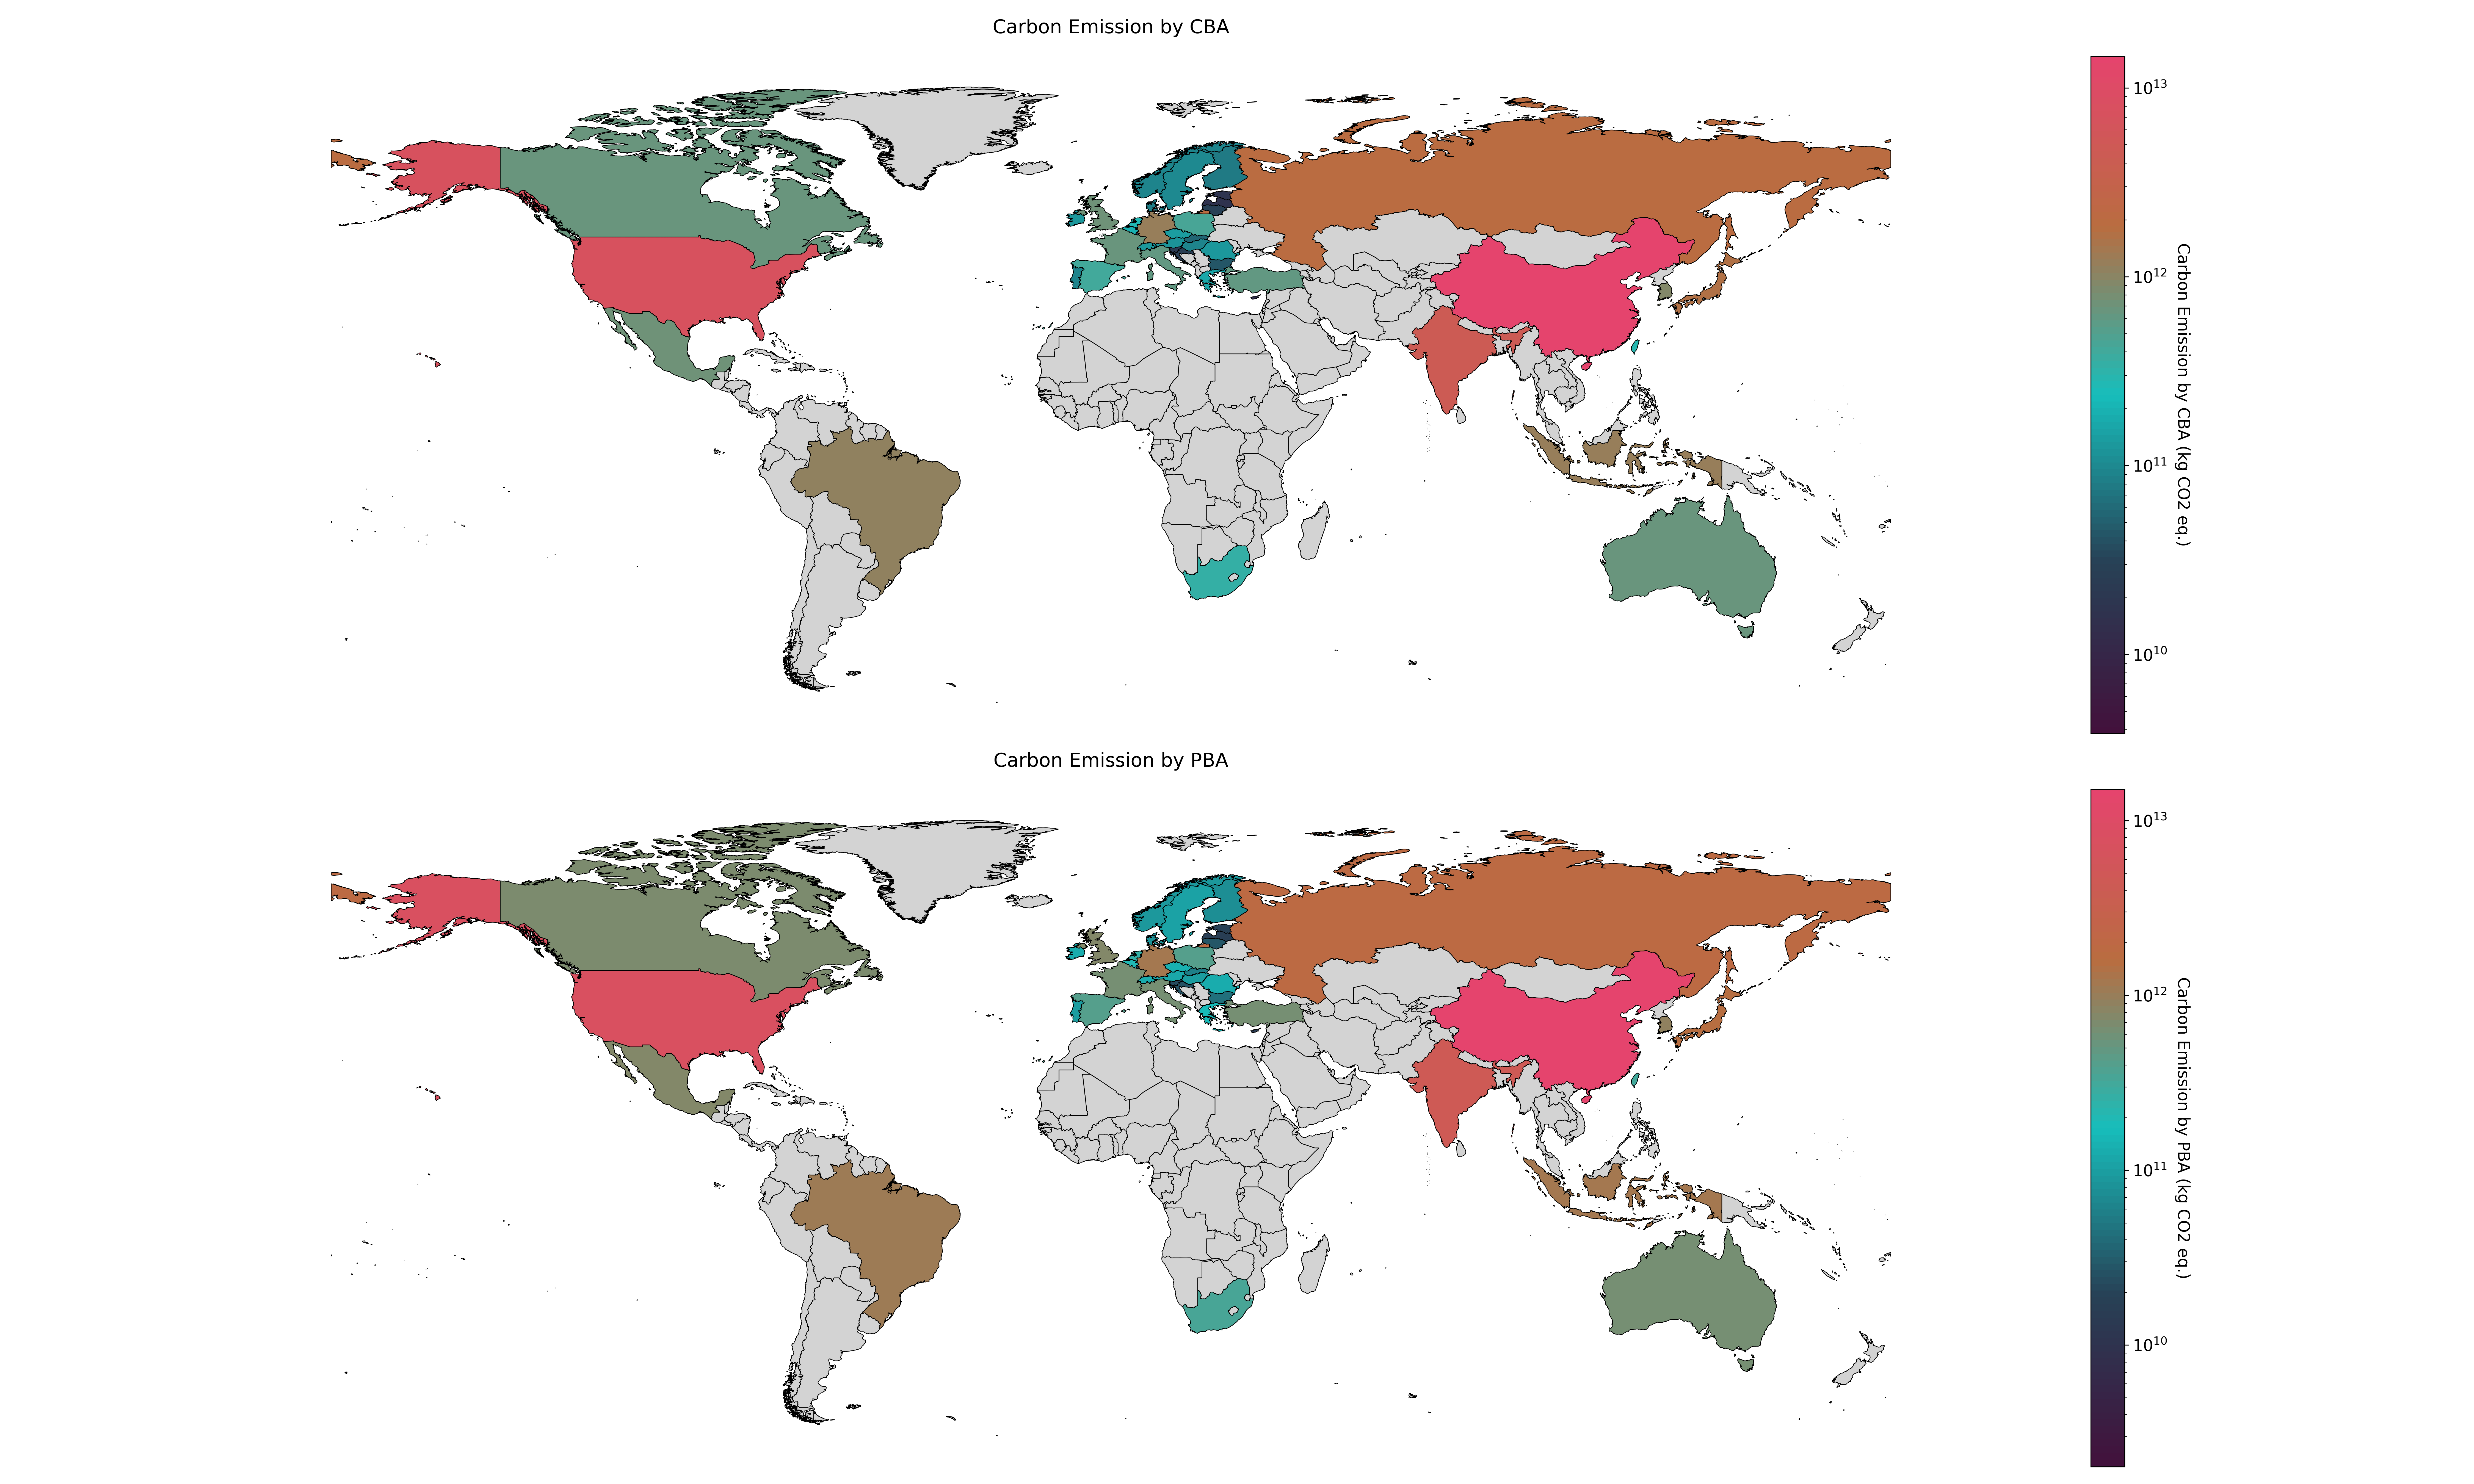
\includegraphics[width=\linewidth]{figures/Graph/Comparison of Carbon Emission (GHG) between PBA and CBA.png}
 \caption{Comparison of Carbon Emission (GHG) between PBA and CBA}\label{fig:Comparison of Carbon Emission (GHG) between PBA and CBA}
\end{sidewaysfigure}
\fi

\subsection{Carbon Uplift in No Trade Scenario}
In the projected scenario where international trade within the semiconductor industry is completely halted, and nations are required to domestically produce what they formerly imported, the data reveal a nuanced tapegraph of carbon uplift percentages across the globe. Figure \ref{fig:Comparison of Carbon Emission (GHG) by CBA and Carbon Uplift} illustrates a marked increase in emissions for several countries. For example, a nation like Germany shows an uplift of 0.26\%, reflecting its high dependency on semiconductor imports and the significant carbon footprint that domestic production would necessitate. Similarly, South Korea, a major player in semiconductor manufacturing, exhibits a 0.19\% increase, which could be attributed to the energy-intensive processes involved in semiconductor fabrication.

On the other end of the spectrum, countries like Saudi Arabia and Russia demonstrate a decrease in carbon emissions, by 0.22\% and 0.35\%, respectively. This surprising trend suggests a possible current overcapacity or a more carbon-efficient domestic production that could replace imports with lower emissions.

Furthermore, the United States, which occupies a central position in the global semiconductor supply chain, shows a potential uplift of 0.29\%, a significant figure given the scale of the country's economy. Meanwhile, China, with its extensive manufacturing infrastructure, sees an uplift of 0.12\%. This lower relative increase may be indicative of its already substantial domestic production capabilities.

The data also bring to light the variable effects on smaller economies such as those in Southeast Asia, where the percentage change swings widely, from a decrease of 0.18\% in countries like Singapore to an increase of 0.31\% in others like Vietnam. These variations emphasize the differing levels of reliance on the global trade of semiconductors and the disparity in carbon emission changes that would result from a shift to self-sufficiency.

This portrayal of carbon uplift, drawn from the dataset, provides a detailed account of the anticipated repercussions on global carbon emissions in the absence of semiconductor trade. It underscores the extent to which international commerce is interwoven with environmental impacts and highlights the potential increase in global carbon footprint that could follow from a turn towards national production in the semiconductor industry.
\ifincludefigures
\begin{sidewaysfigure}
  \centering
  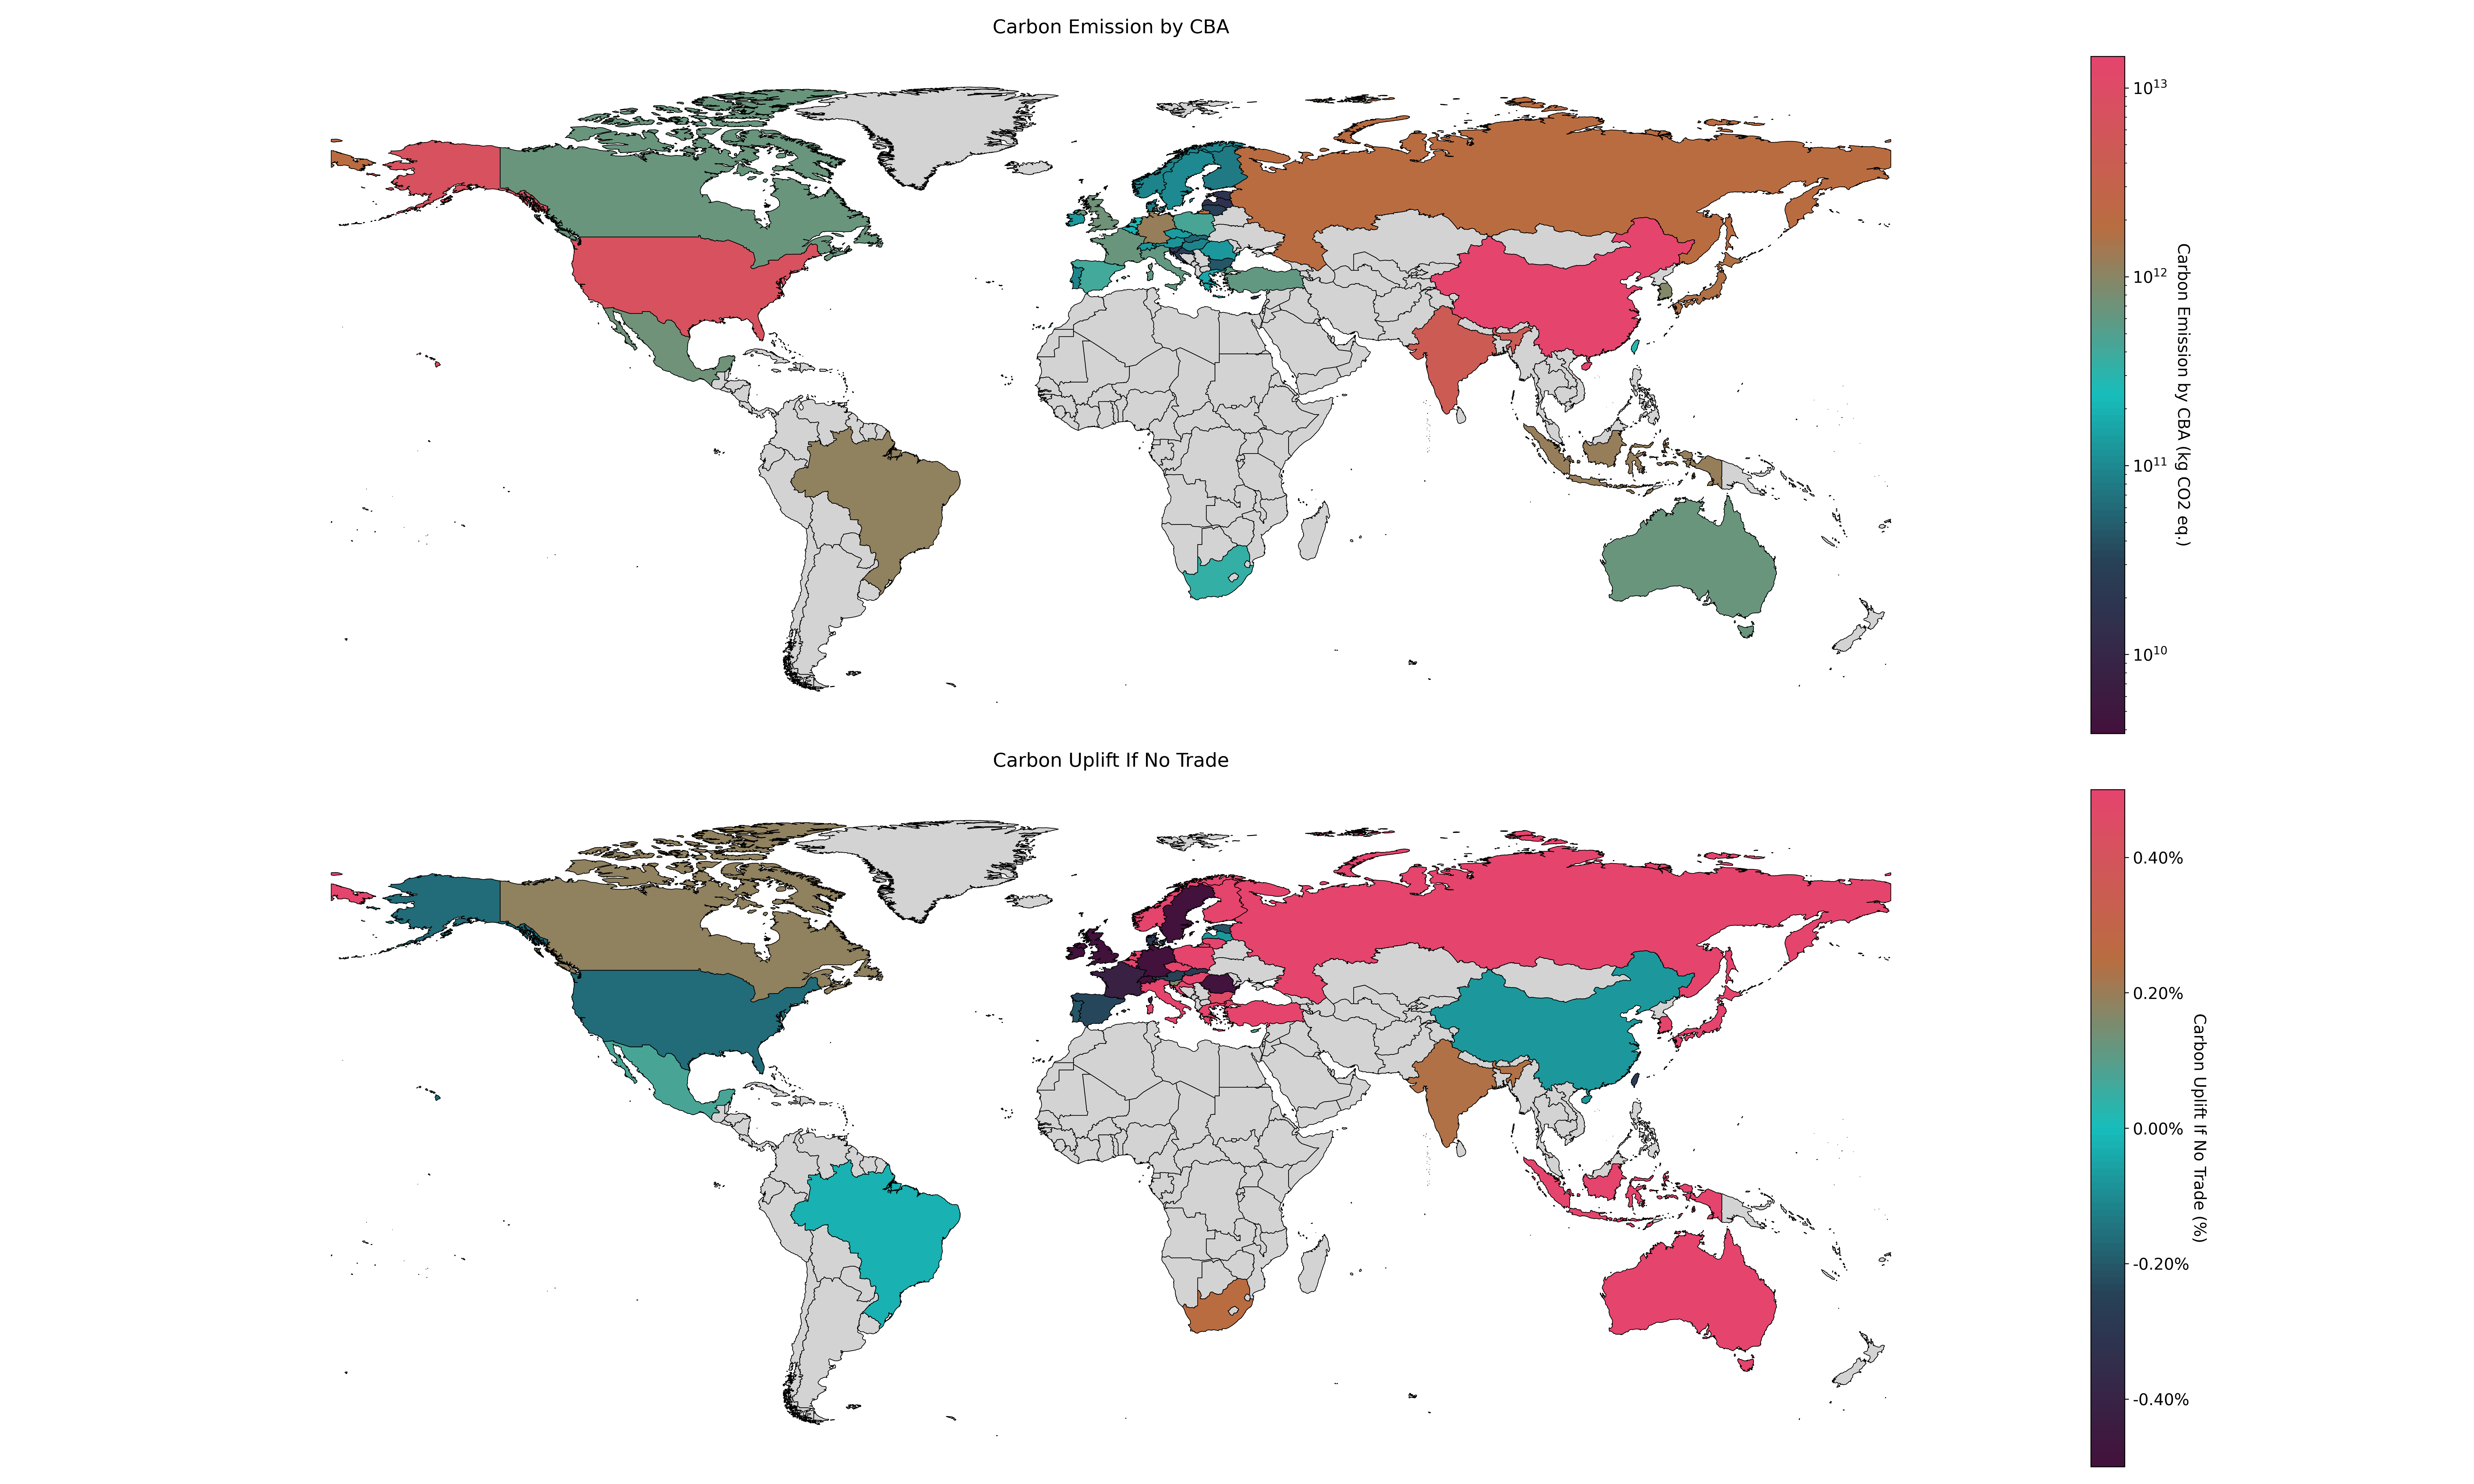
\includegraphics[width=\linewidth]{figures/Graph/Comparison of Carbon Emission (GHG) by CBA and Carbon Uplift.png}
 \caption{Comparison of  Carbon Emission (GHG) by CBA and Carbon Uplift}\label{fig:Comparison of  Carbon Emission (GHG) by CBA and Carbon Uplift}
\end{sidewaysfigure}
\fi

In the compendium of these findings, Figure \ref{fig:Value of Carbon Uplift If No Trade Heatmap in 2022} manifests the hypothetical variance in carbon emissions contingent upon the cessation of trade, particularly within the semiconductor industry's supply chain. The sectors scrutinized are dissected into two principal echelons—upstream and downstream—each critical to the lifecycle of semiconductor production.

In the upstream ambit, the data convey that for ``Other non-ferrous metal ores and concentrates'' China's carbon uplift is approximately -0.053\%, a fractional decrement. The United States records a similar downtrend at -0.045\%. For 'secondary other non-ferrous metals for treatment" both nations effectively exhibit no change, as indicated by the negligible uplift values close to zero.

The downstream analysis for ``Electrical machinery and apparatus n.e.c. (31)'' and ``Office machinery and computers (30)'' denotes a -0.023\% and -0.006\% carbon uplift for China, respectively. The United States reflects a more pronounced -0.050\% reduction in the ``Electrical machinery'' sector and a slight increase of 0.004\% in the ``Office machinery'' sector. The slight increase for the U.S. in the ``Office machinery'' sector diverges from the overall downward trend observed in other sectors.

``Radio, television and communication equipment and apparatus (32)'' sees an uplift of approximately 0.003\% for China, contrasting with a -0.030\% reduction for the United States. For ``Medical, precision and optical instruments, watches and clocks (33)'' China's figures suggest a -0.023\% decrease, while the United States presents a -0.033\% reduction.

When evaluating the aggregated data for all semiconductor-related products, China showcases a carbon uplift of -0.077\% across related products, -0.028\% for upstream, and -0.049\% for downstream products. The United States, however, reveals a more substantial decrease across these categories, with -0.168\% for related products, -0.059\% for upstream, and -0.109\% for downstream sectors.

These percentages suggest that in the hypothetical scenario of a no-trade environment, both China and the United States would experience a decrease in carbon emissions across most semiconductor sectors, with the United States displaying a marginally greater reduction. This trend aligns with the broader global efforts to achieve carbon neutrality, yet it underscores the criticality of trade in optimizing the carbon efficiency of the semiconductor supply chain.

Conversely, many other countries may rely heavily on the import of semiconductors and related products, lacking the same level of infrastructure or technological prowess. If these nations were compelled to produce semiconductors domestically, they might need to invest in new facilities and processes, which could be less efficient and more carbon-intensive than those available in countries like China and the United States. Additionally, the scale of production could affect emissions; smaller-scale operations may not benefit from the same efficiencies as larger ones.

Moreover, the overall increase in global carbon emissions reflects the intricate and optimized nature of the current global trade network. Specialized production and economies of scale in certain regions lead to a reduced carbon footprint per unit of output. When this specialization is absent, as in a no-trade scenario, production may become less efficient globally, leading to higher carbon emissions.

This interplay of regional specialization, technological disparities, and economies of scale forms the crux of the potential increase in global carbon emissions in the absence of trade. The heatmap, while highlighting the outliers in China and the United States, simultaneously reveals that the global picture is one of increased carbon output, underlying the critical role of trade in not only economic efficiency but also in the pursuit of environmental sustainability.
\ifincludefigures
\begin{figure}
 \centering
 \makebox[\textwidth][c]{\includegraphics[width=1\textwidth]{figures/Graph/Value of Carbon Uplift If No Trade Heatmap in 2022.png}}
 \caption{Value of Carbon Uplift If No Trade Heat Map in 2022}\label{fig:Value of Carbon Uplift If No Trade Heatmap in 2022}
\end{figure}
\fi

\subsection{Carbon Uplift in No Sino-US Trade Scenario}

In the examination of the projected carbon uplift in the hypothetical scenario of no trade between China and the United States, we unveil distinct patterns within the semiconductor industry's upstream and downstream sectors. This analysis is predicated on the percentage change in carbon emissions, encapsulated within the data points provided.

For the upstream sector, ``Other non-ferrous metal ores and concentrates'' the data reflects a negligible decrease in emissions for China at approximately -0.0001\%, and an increase for the United States at approximately 0.0047\%. In the adjacent sector of 'secondary other non-ferrous metals for treatment" both nations appear to maintain an invariant emission level, suggested by the uplift values insignificantly close to zero.

Within the realm of precious metals, China's emissions present a slight increase of 0.0041\%, while the United States exhibits a more significant decrease of -0.0101\%. The data for ``secondary precious metals for treatment'' remains effectively unchanged for both countries, akin to the pattern observed in the 'secondary other non-ferrous metals for treatment" sector.

Delving into the downstream sectors, ``Electrical machinery and apparatus n.e.c. (31)'' for China shows a reduction in emissions by -0.0005\%, contrasted by an increase of 0.0093\% for the United States. For ``Office machinery and computers (30)'' China's carbon uplift is -0.0003\%, whereas the United States sees an augmentation by 0.0172\%. ``Radio, television and communication equipment and apparatus (32)'' records a decrease for both countries, with China at -0.0002\% and the United States at -0.0053\%. The sector of ``Medical, precision and optical instruments, watches and clocks (33)'' exhibits a decrease in emissions for China by -0.0023\ and an increase for the United States by 0.0054\%.

Aggregating the sectors under ``semiconductivity Related Products'' China demonstrates a slight increase of 0.0114\%, while the United States shows a notable increase of 0.0212\%. In ``semiconductivity Upstream Products'' both countries experience an increase, with China at 0.0041\% and the United States at -0.0054\%. For 'semiconductivity Downstream Products" China shows a decrease of -0.0029\%, and the United States a more significant increase of 0.0266\%.

The variegated data implicates that in the absence of bilateral trade, both China and the United States would experience a mix of increases and decreases in carbon emissions across different sectors. The United States, in particular, shows larger percentage changes both in terms of decreases and increases. This disparity likely stems from the comparative advantage inherent within each nation's industrial complex, emphasizing the nuanced interdependence between the two superpowers within the global semiconductor market.

It is this delicate equilibrium of trade, production efficiencies, and carbon emissions that Figure \ref{fig:Value of Carbon Uplift If No Sino-US Trade Heatmap in 2022} strives to visually articulate. The color-coded cells, each corresponding to a unique data point, reveal a tapestry of potential outcomes that are instrumental in contextualizing the environmental implications of trade policies within the semiconductor industry.
\ifincludefigures 
\begin{figure}
 \centering
 \makebox[\textwidth][c]{\includegraphics[width=1\textwidth]{figures/Graph/Value of Carbon Uplift If No Sino-US Trade Heatmap in 2022.png}}
 \caption{Value of Carbon Uplift If No Sino-US Trade Heat Map in 2022}\label{fig:Value of Carbon Uplift If No Sino-US Trade Heatmap in 2022}
\end{figure}
\fi
\subsection{Carbon Uplift in No Sino-US with Gaming Trade Scenario}

Figure \ref{fig:Value of Carbon Uplift If No Sino-US with Gaming Trade Heatmap in 2022} provided delineates the carbon uplift, articulated as a direct consequence of a trade rearrangement modeled on game-theoretic principles for the year 2022. This analysis illuminates the carbon footprint repercussions in various industrial sectors, with a spotlight on semiconductivity.

For China, the data indicates a notable carbon uplift of 1.2301\% in the semiconductivity related products sector. This represents a significant environmental benefit accruing from the hypothetical trade reallocation. Conversely, there is a marginal contraction of -0.0148\% in the semiconductivity upstream products, counterbalanced by an uplift of 0.3482\% in the downstream products.

The United States displays a more modest uplift of 0.0773\% in semiconductivity related products, suggesting a lesser but still positive environmental impact from the trade redistribution. A negligible decrease of -0.0013\% is observed in the upstream products, while downstream products experience an uplift of 0.1903\%.

Globally, the analysis reflects a carbon uplift of 0.3568\% in semiconductivity related products, with a slight decrease of -0.0043\% in the upstream sector. The downstream sector sees an uplift of 0.1229\%, underscoring the significant environmental impacts within the semiconductor supply chain on a global scale.

Such data exemplifies the critical role of trade patterns in shaping carbon emission trajectories. It reveals that strategic trade reallocations can potentially lead to an enhancement or deterioration of environmental outcomes, particularly within high-tech and high-impact sectors like semiconductivity.

This granular perspective allows us to infer not only the environmental implications of these strategic decisions but also the differential impacts that such redistributions might engender across various production stages. It emphasizes the need for an integrated approach to trade policy, one that takes into account the complex interdependencies within global supply chains and their environmental ramifications.
\ifincludefigures
\begin{figure}
  \centering
  \makebox[\textwidth][c]{\includegraphics[width=1\textwidth]{figures/Graph/Value of Carbon Uplift If No Sino-US with Gaming Trade Heatmap in 2022.png}}
  \caption{Value of Carbon Uplift If No Sino-US with Gaming Trade Heatmap in 2022}\label{fig:Value of Carbon Uplift If No Sino-US with Gaming Trade Heatmap in 2022}
 \end{figure}
\fi
\section{How does Semi-conductor Related Products Trade Impact Global Carbon Emissions}

\subsection{Carbon Uplift in No Semi-conductor Related Products Trade Scenario}

Figure \ref{fig:Carbon Uplift If No Trade 2022} displays the percentage change in carbon emissions in the scenario of no semiconductor trade, segregated into three categories: related products, upstream products, and downstream products.

The global percentage change in carbon emissions for semiconductivity related products shows an increase, indicating that on a worldwide scale, ceasing trade in this category would lead to an uptick in emissions due to domestic production.

However, some countries like the United States and China exhibit a decrease in carbon emissions across all three sectors. This could suggest that these countries are currently producing these goods more efficiently than the global average, and shifting to domestic production exclusively might actually decrease their carbon emissions in these categories.

For example, the United States shows a decrease of 0.2495\% in related products, a decrease of 0.1300\% in upstream products, and a decrease of 0.1195\% in downstream products. Similarly, China's data indicates a decrease of 0.2070\% in upstream products and a 0.0184\% decrease in downstream products, which may reflect the high efficiency and scale of their existing semiconductor manufacturing capabilities.

On the other hand, for countries where an increase is observed, such as those that might be more import-reliant for these products, the need to develop or expand domestic production may lead to higher emissions compared to the current state of trade.

The specific increases or decreases in the respective sectors for each country will guide us in understanding the potential environmental impact of shifts in the semiconductor trade policy and production landscape. It is important to note that these figures are subject to the nuances of each country's existing industrial capabilities and the complexity of the semiconductor supply chain. 
\ifincludefigures 
\begin{figure}
 \centering
 \makebox[\textwidth][c]{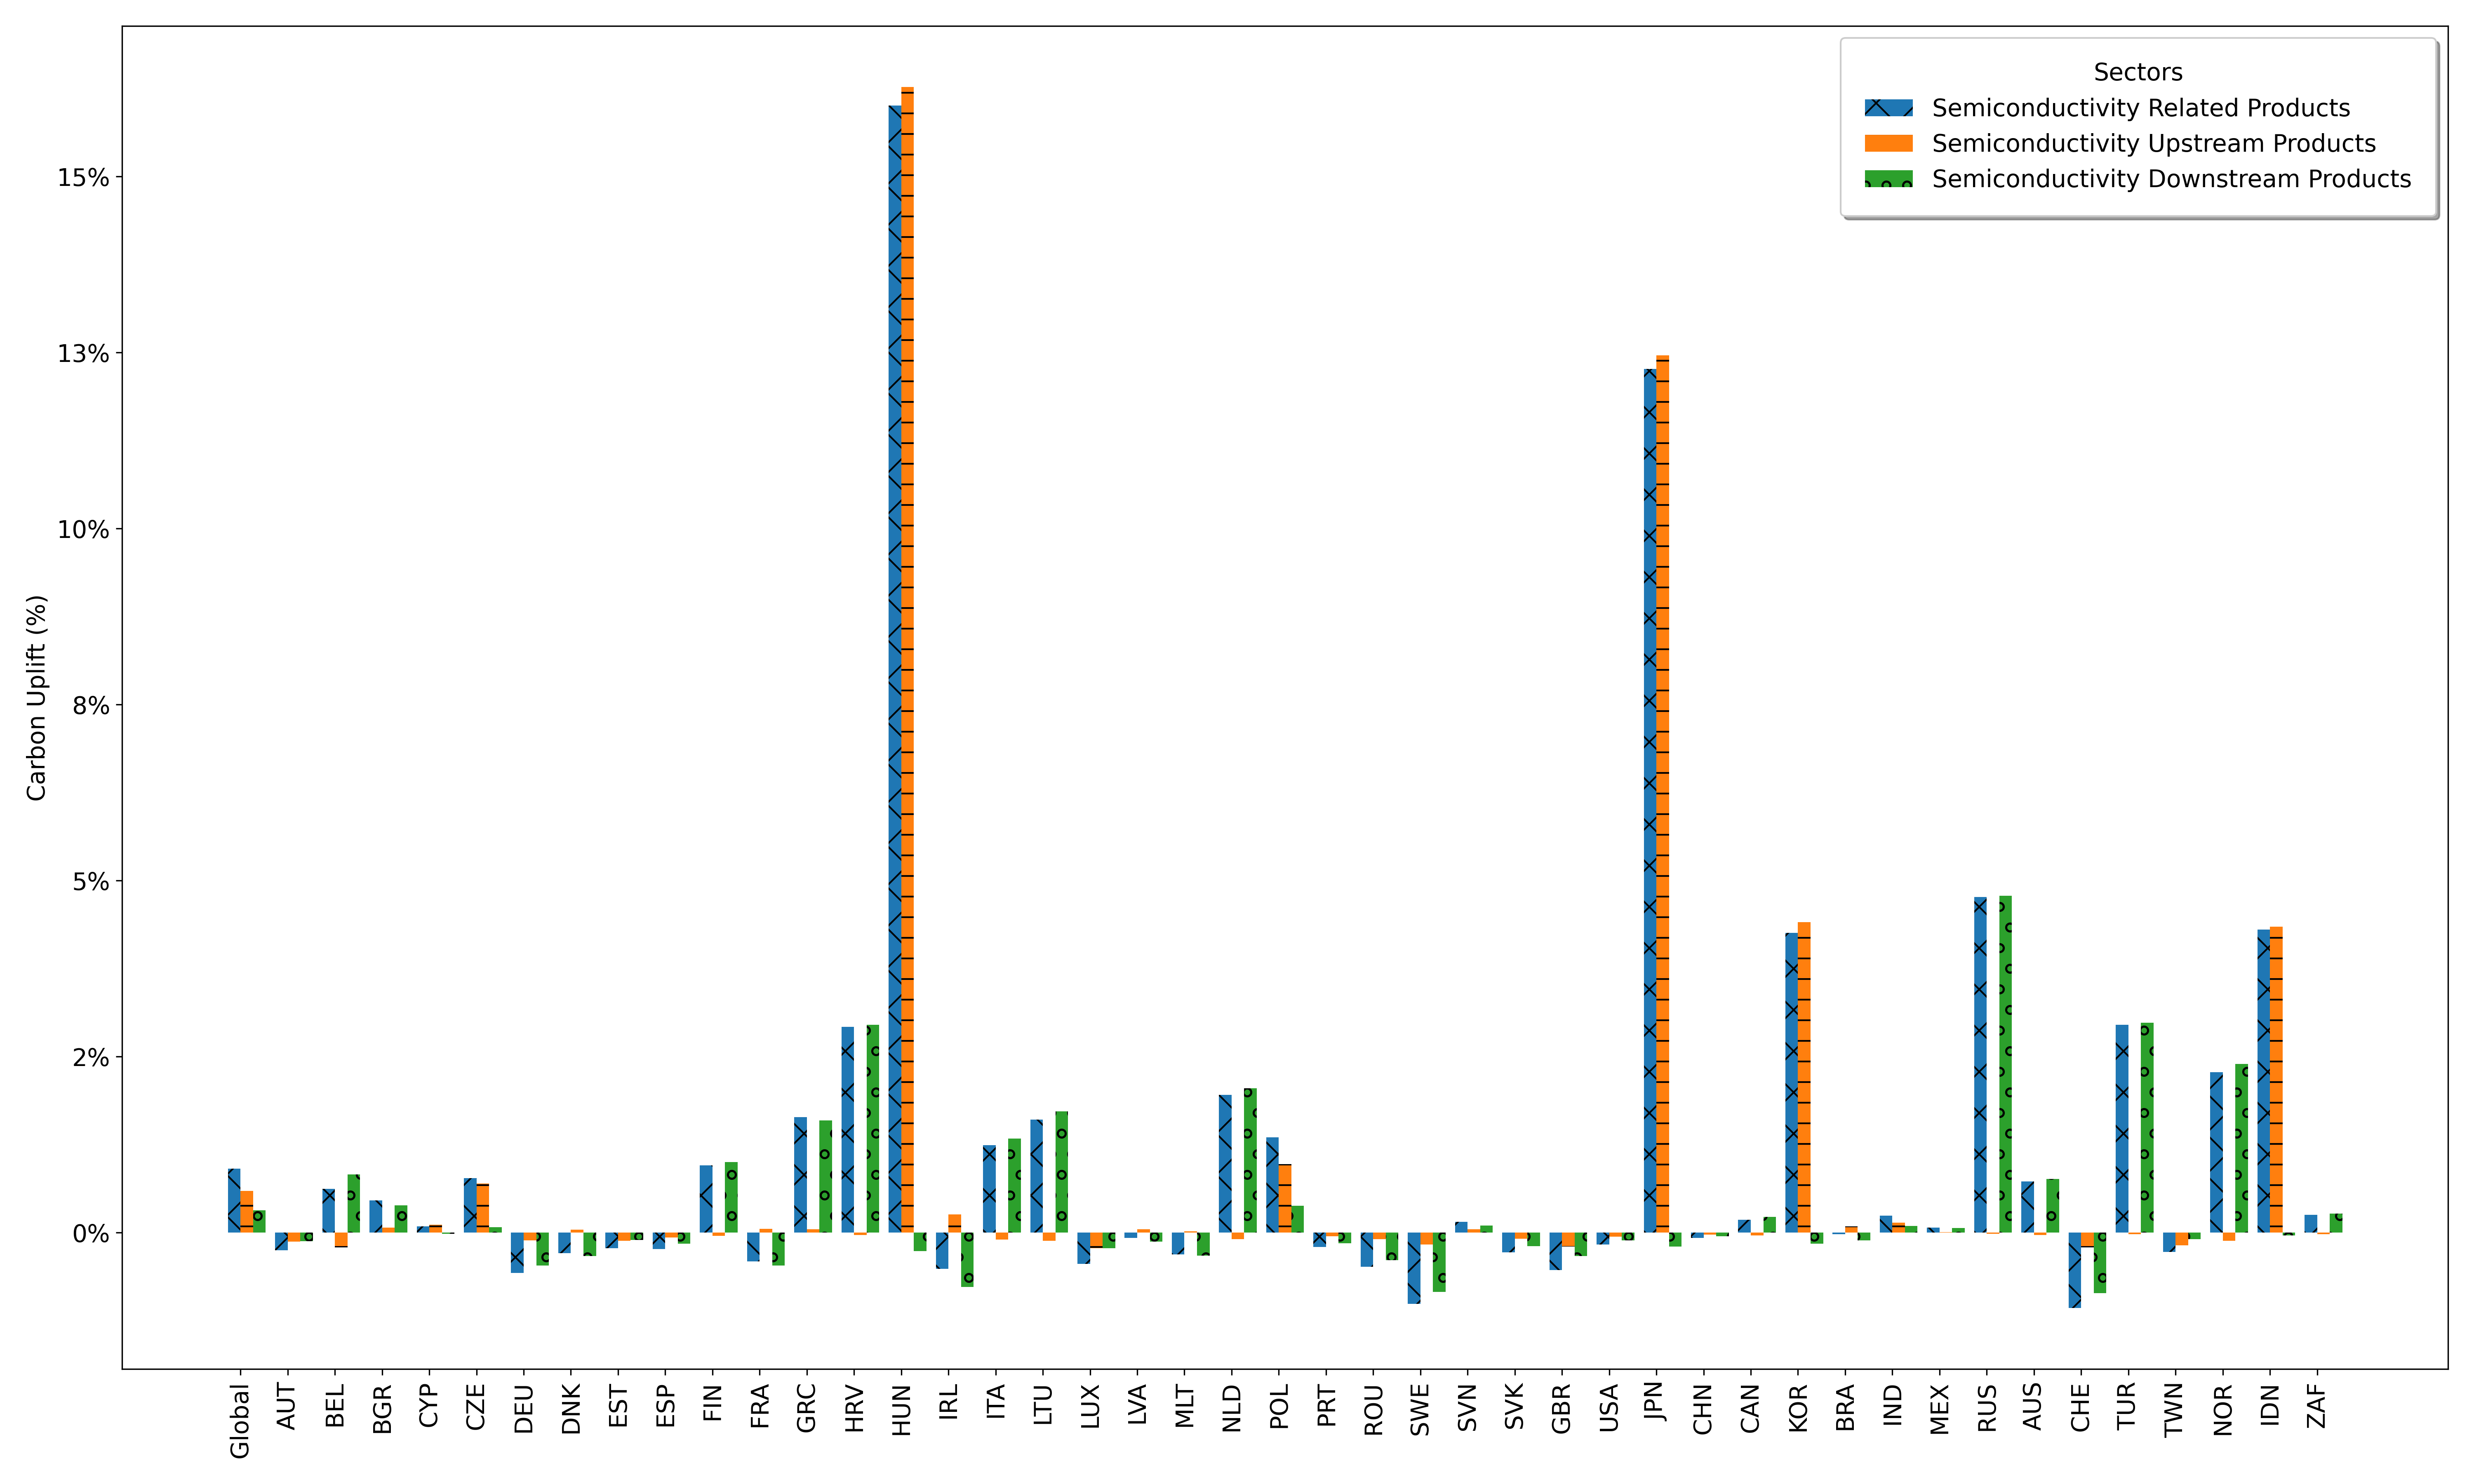
\includegraphics[width=1\textwidth]{figures/Graph/Carbon Uplift If No Trade 2022.png}}
 \caption{Carbon Uplift If No Trade 2022}\label{fig:Carbon Uplift If No Trade 2022}
\end{figure}
\fi
Figure \ref{fig:Carbon Uplift Trends If No Trade(2000-2022)} meticulously plots the trajectory of carbon emission changes under a theoretical framework where no trade exists. Focusing on the semiconductor industry, the data is bifurcated into related, upstream, and downstream products over a span of two decades, encapsulating the temporal evolution of carbon uplift percentages for both China (CN) and the United States of America (US).

From the dawn of the millennium in 2000, we observe China's carbon uplift in semiconductivity related products initiating at approximately 0.0348\%, with a shift towards a reduction in emissions across all sectors by 2022, landing at -0.0768\%. Notably, the trajectory exhibits a downward trend, punctuated by fluctuating increments, particularly evident in the upstream products sector, which sees an initial increase to 0.0257\% in 2000, followed by a decrease to -0.0279\% by 2022. The downstream products sector for China reflects this decrement more modestly, from 0.0091\% in 2000 to -0.0488\% in 2022.

The United States presents a distinct pattern; the carbon uplift in semiconductivity related products starts at -0.0425\% in 2000 and deepens to -0.1678\% by 2022. This significant downward trajectory suggests an increasing efficiency in carbon emissions over time. The upstream sector undergoes a remarkable decrease from -0.0244\% in 2000 to -0.0590\% in 2022, emphasizing a consistent focus on reducing carbon intensity. The downstream sector echoes this trend, commencing at -0.0181\% in 2000 and culminating at -0.1088\% in 2022, underscoring the role of technological advancements and efficiency improvements.

In the broader global context, the carbon uplift exhibits an overall escalation, suggesting that while individual nations such as China and the United States may optimize and reduce their carbon footprint, the aggregate global emissions could potentially rise in the absence of international trade. This scenario accentuates the integral role of global trade mechanisms in distributing the production of semiconductors to locations where carbon efficiency is maximized.

The data, set against the backdrop of the intricate interactions of the semiconductor industry's global supply chain, serves as an empirical testament to the environmental implications of trade policies and the technological evolutions within this pivotal sector. As the author of this analysis, the intent is not only to present these data points but also to foster a dialogue on the role of international cooperation in mitigating carbon emissions, underpinning the necessity of a symbiotic approach to trade and environmental sustainability.
\ifincludefigures
\begin{figure}
\centering
\makebox[\textwidth][c]{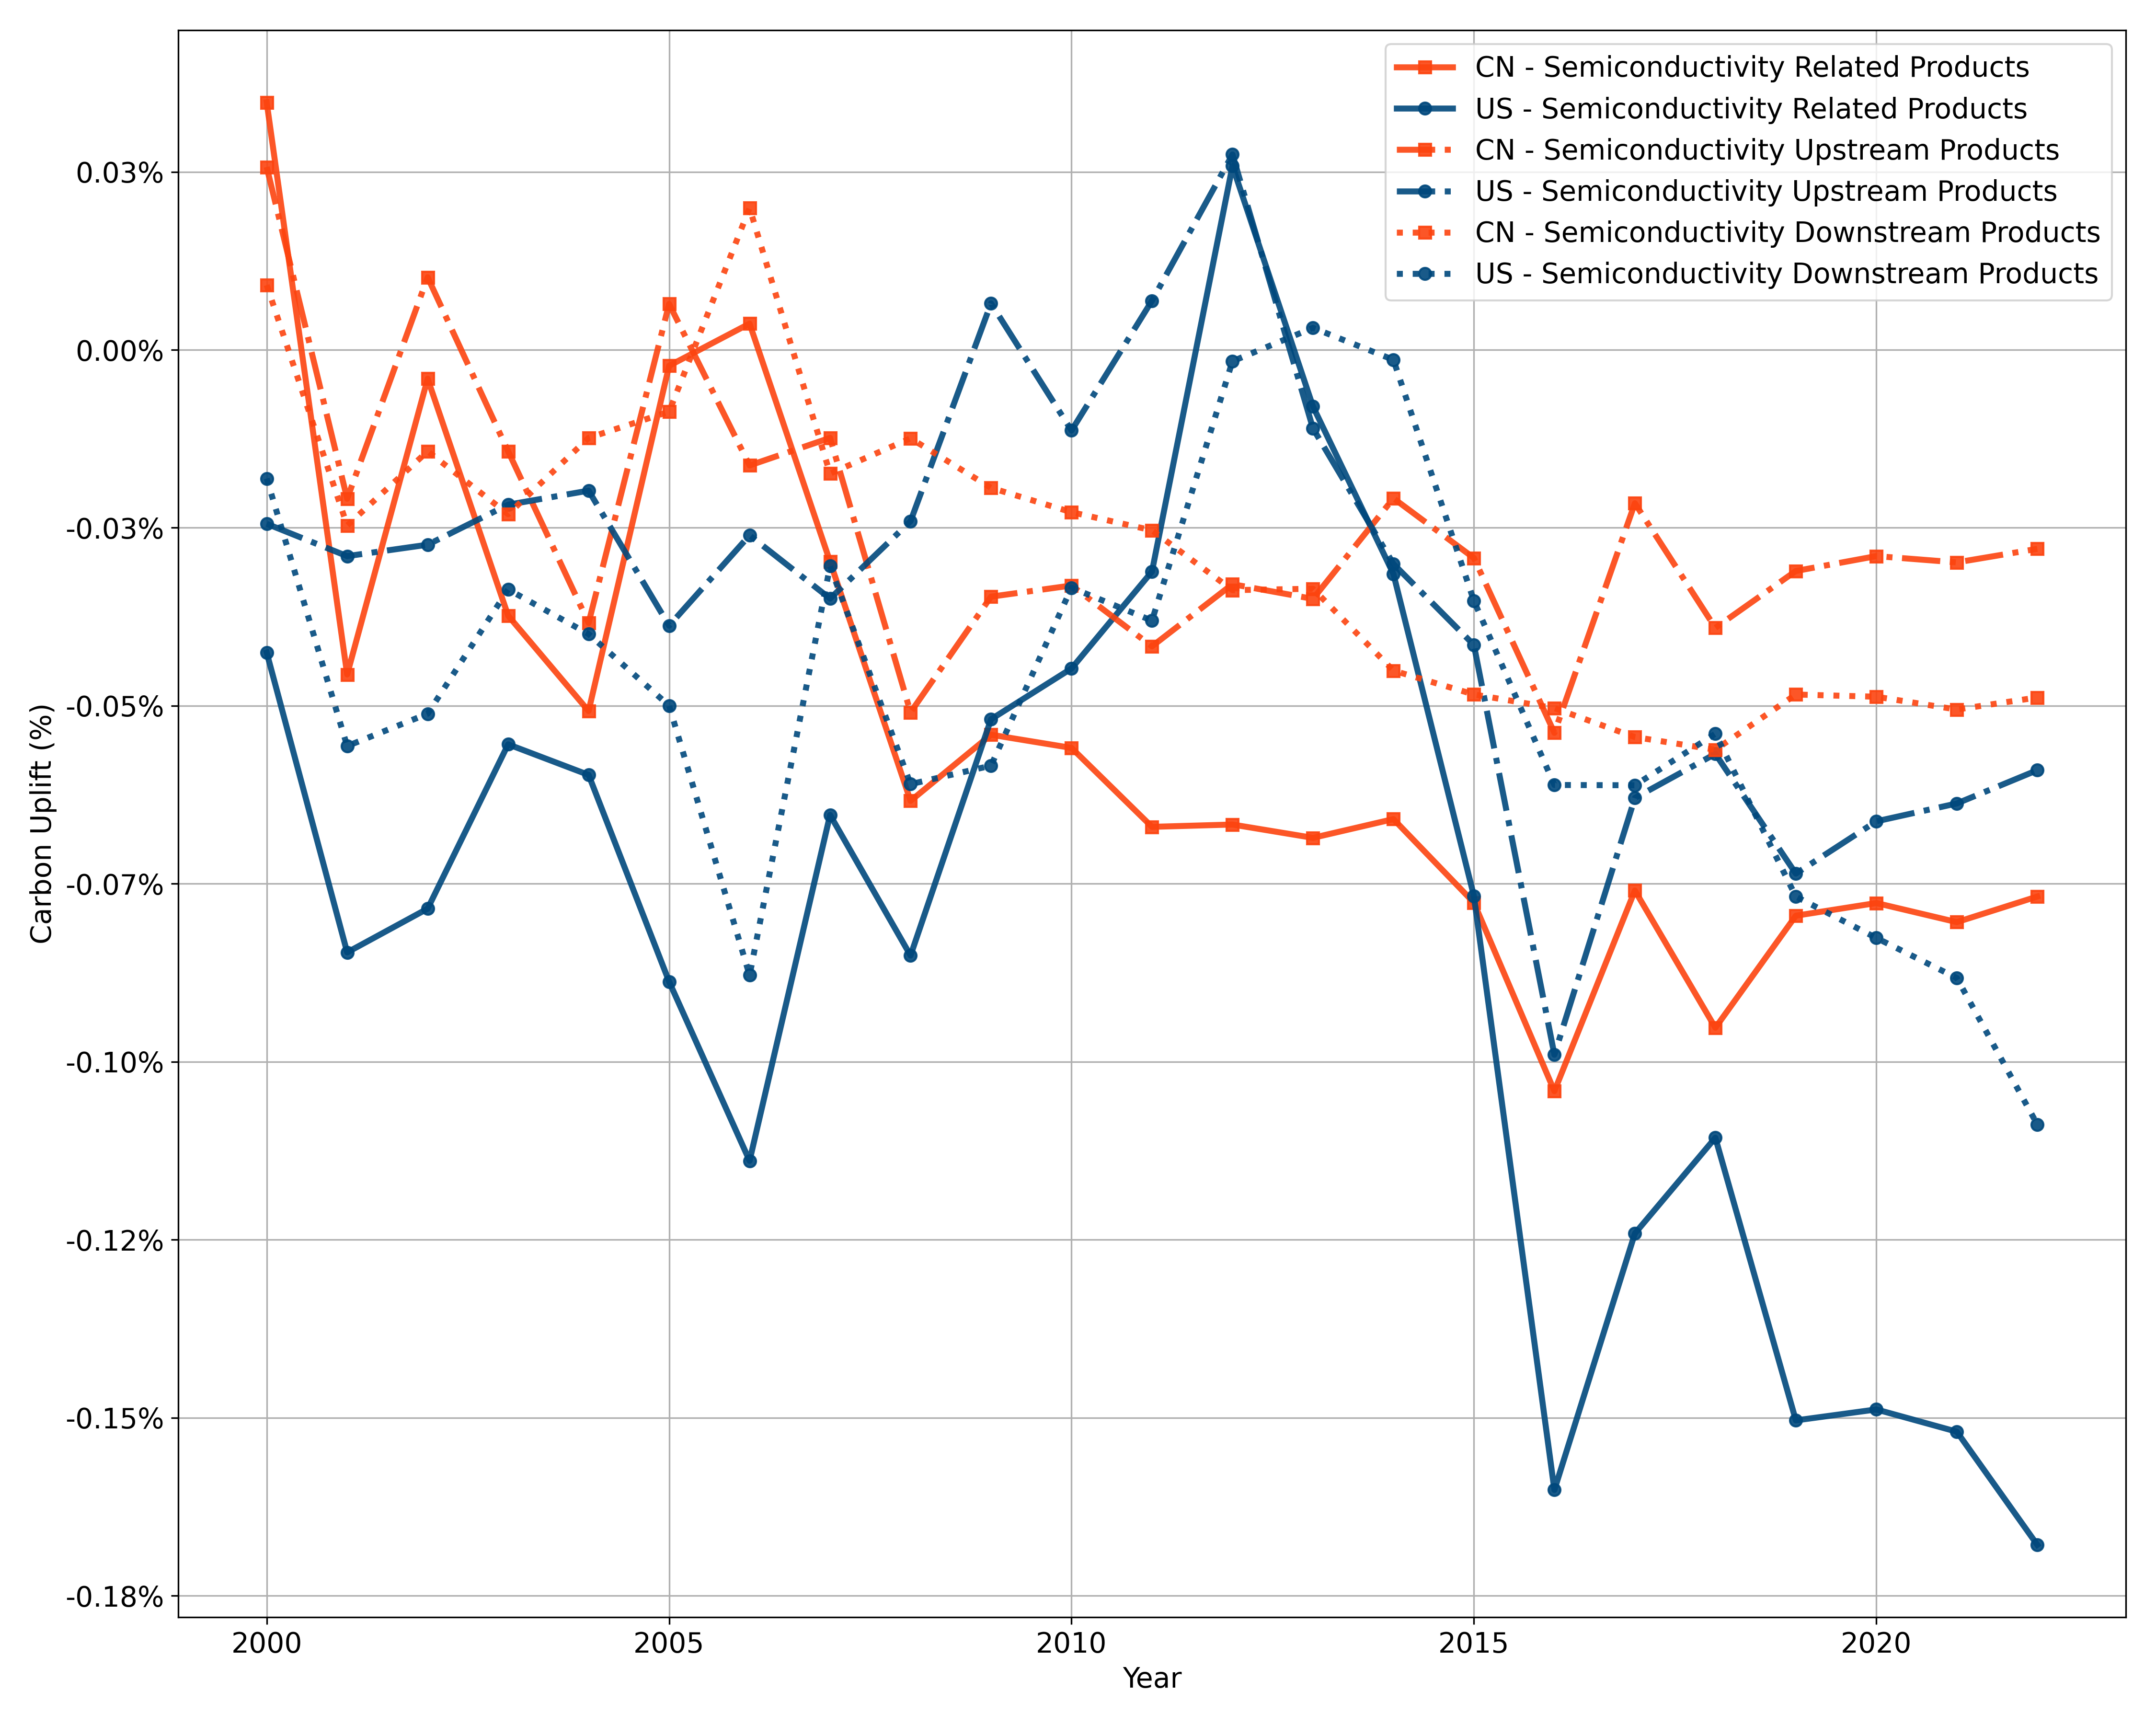
\includegraphics[width=1\textwidth]{figures/Graph/Carbon Uplift Trends If No Trade(2000-2022).png}}
\caption{Carbon Uplift Trends If No Trade(2000-2022)}\label{fig:Carbon Uplift Trends If No Trade(2000-2022)}
\end{figure}
\fi
\subsection{Carbon Uplift in No Sino-US Semi-conductor Related Products Trade Scenario}


The comparative analysis of carbon emission uplift under no trade scenarios, globally and between China and the United States, Figure \ref{fig:Comparison of Carbon Uplift between No Trade Scenario and No Sino-US Trade Scenario} provides pivotal insights into the environmental repercussions of trade policies. In a no-trade environment, the assumption is that previously imported goods are entirely substituted by domestic production, leading to an increase in carbon emissions due to the shift in production dynamics.

Globally, the absence of trade would result in a carbon uplift of 0.9106\% for semiconductivity-related products, 0.5956\% for upstream products, and 0.3152\% for downstream products. This indicates a not insignificant surge in emissions, positing that the global market relies on trade to maintain lower carbon output levels through more efficient production distributions.

In contrast, China shows a reduction in carbon uplift across all categories when trade is absent, with -0.0768\% for related products, -0.0280\% for upstream, and -0.0488\% for downstream sectors. This can be interpreted as China's industrial sector possibly benefiting from the import of less carbon-intensive goods, or indicating a high efficiency in certain domestic productions that would otherwise be replaced by imports.

The United States presents a different picture, with a substantial carbon uplift reduction when trade is eliminated: -0.1678\% for related products, -0.0590\% for upstream, and -0.1088\% for downstream sectors. This suggests that the U.S. may be offloading more carbon-intensive production to trade partners and would see an environmental benefit in terms of carbon emissions if it were to produce these goods domestically.

When examining the scenario where only Sino-U.S. trade is halted, we observe a minimal global carbon uplift of 0.0031\% for related products, 0.0004\% for upstream, and 0.0026\% for downstream products. This negligible change suggests that while the Sino-U.S. trade relationship is significant, other global trade activities maintain the predominant share of carbon emission contributions.

China's carbon uplift in a no Sino-U.S. trade scenario slightly increases for semiconductivity-related and upstream products, with 0.0011\% and 0.0041\% respectively, yet the downstream sector shows a reduction, reflecting the nuanced impacts across different sectors. For the United States, the absence of bilateral trade with China reveals a carbon uplift of 0.0212\% for related products and a notable increase for downstream products by 0.0266\%, again underscoring the complexity of sector-specific trade impacts on carbon emissions.
\ifincludefigures 
\begin{figure}
 \centering
 \makebox[\textwidth][c]{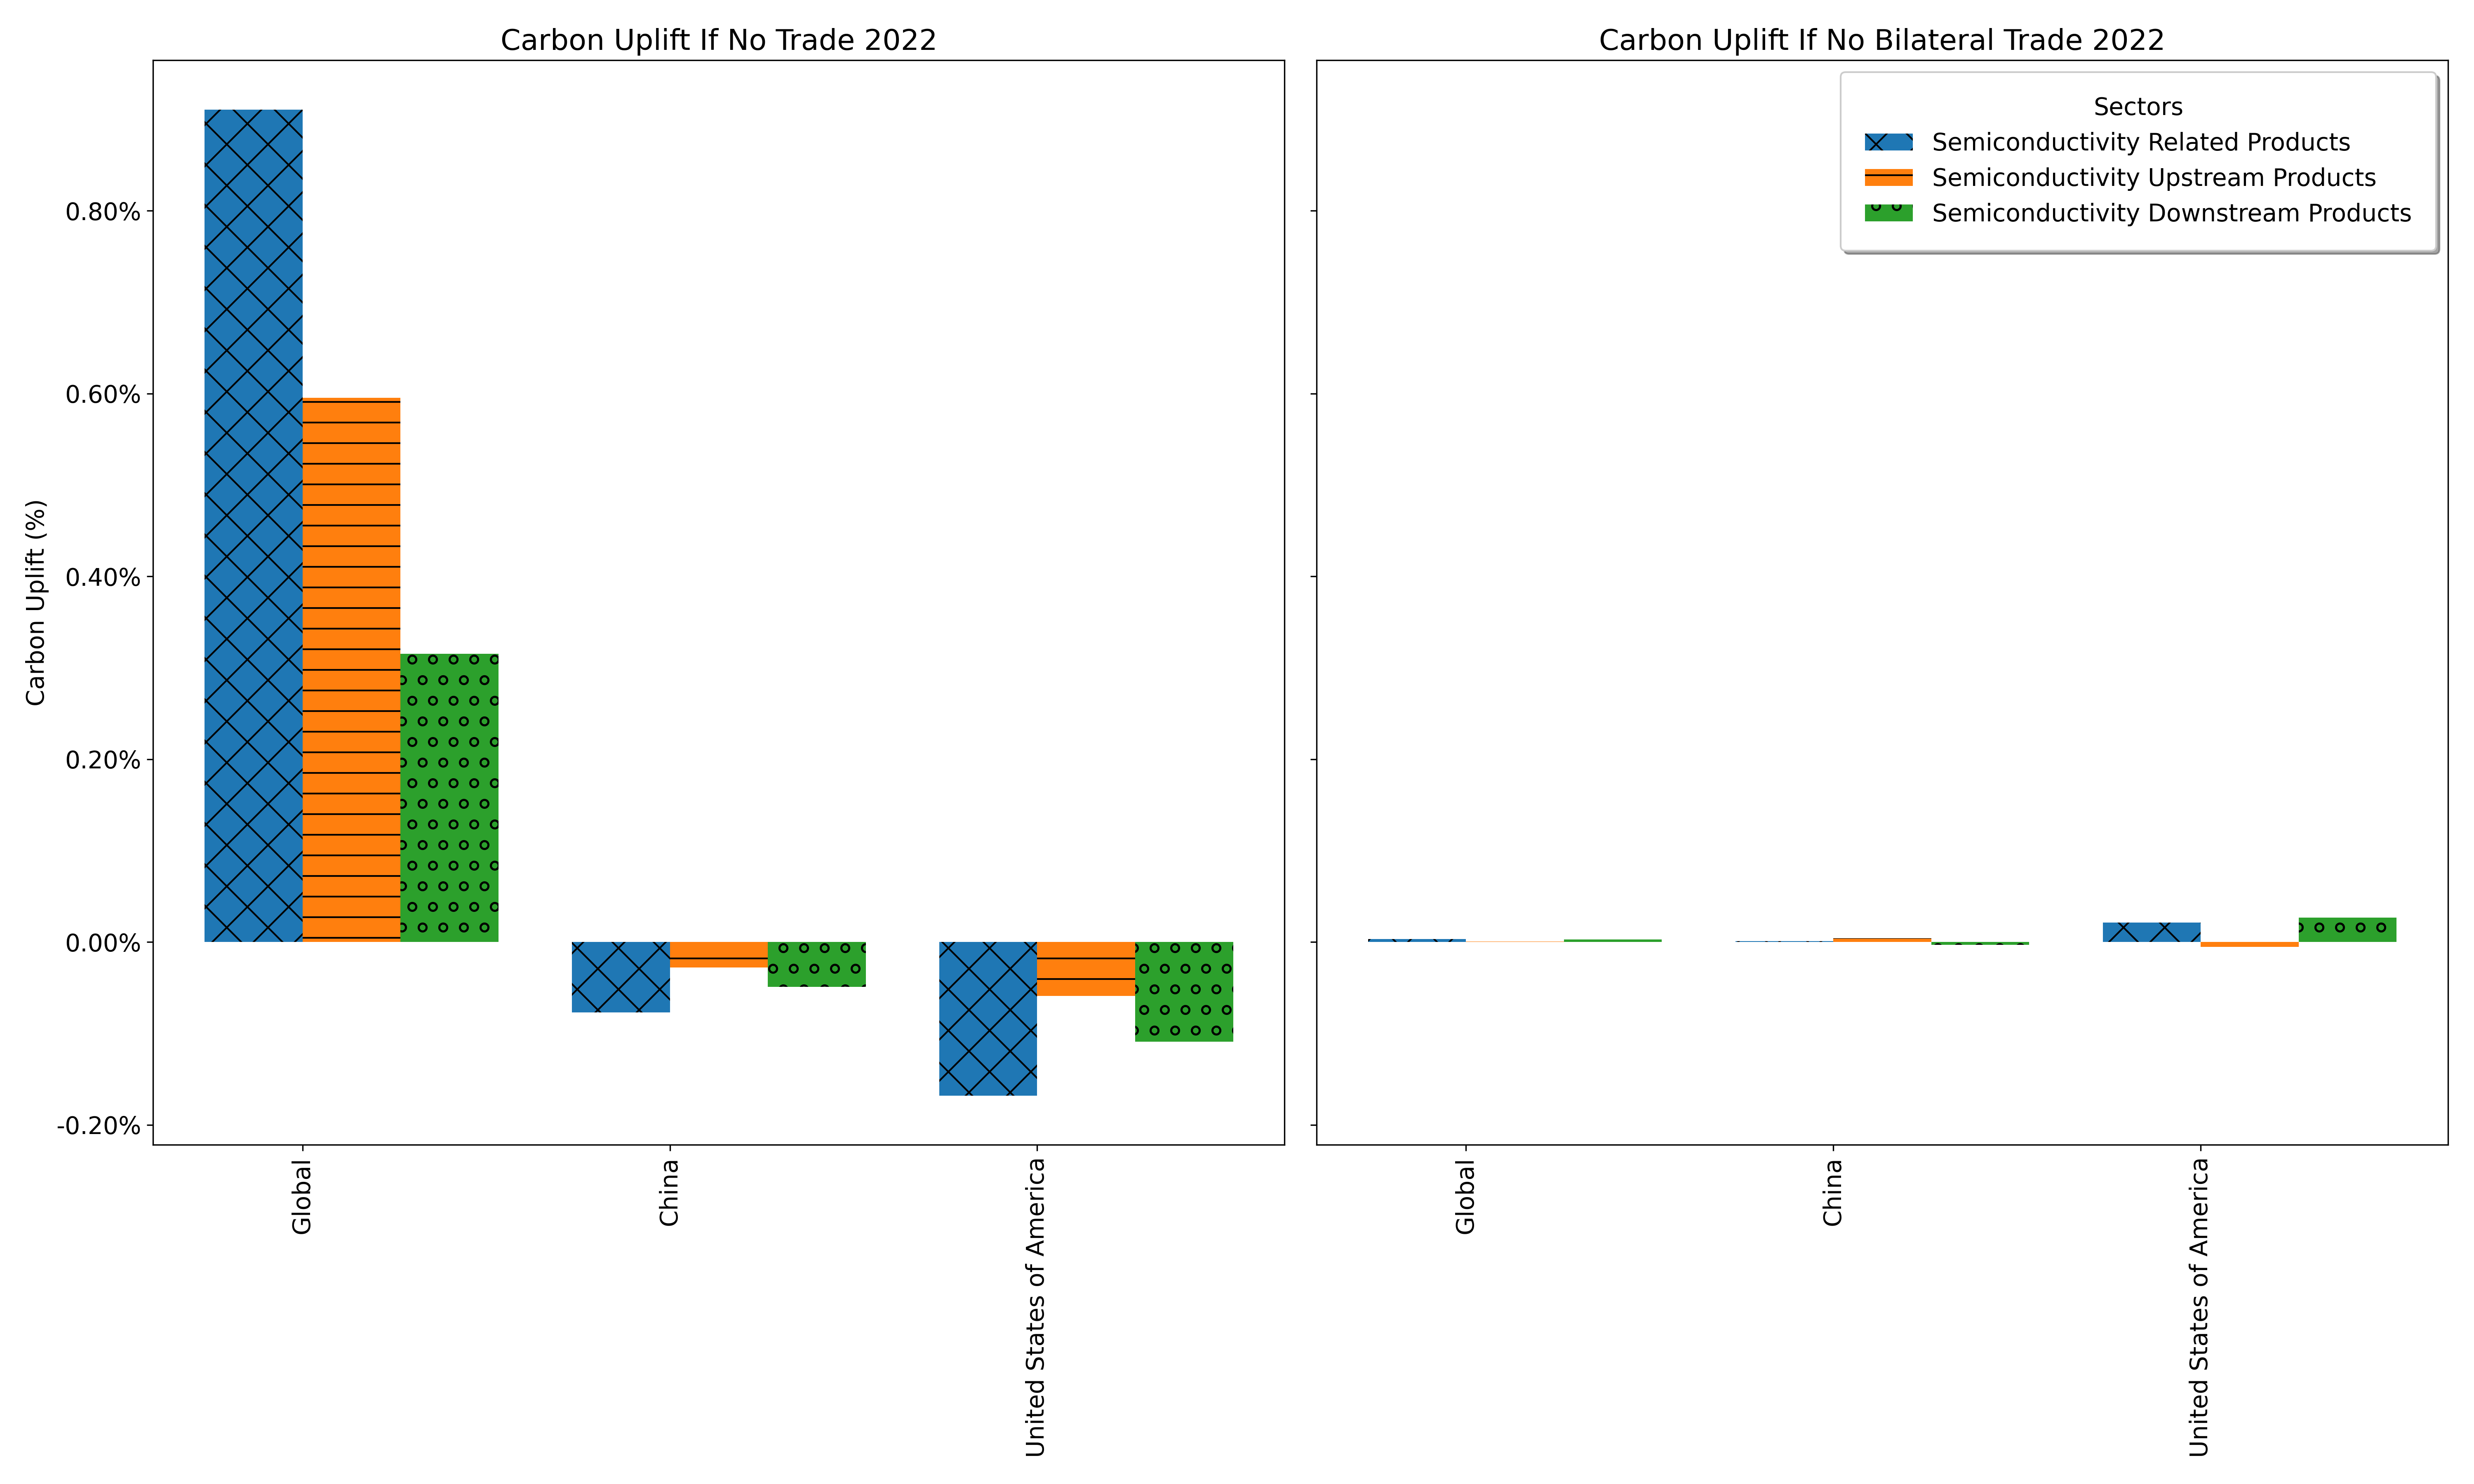
\includegraphics[width=1\textwidth]{figures/Graph/Comparison of Carbon Uplift between No Trade Scenario and No Sino-US Trade Scenario.png}}
 \caption{Comparison of Carbon Uplift between No Trade Scenario and No Sino-US Trade Scenario}\label{fig:Comparison of Carbon Uplift between No Trade Scenario and No Sino-US Trade Scenario}
\end{figure}
\fi
In the analysis presented here, the graph Figure \ref{fig:Carbon Uplift Trends If No Sino-US Trade(2000-2022)} reflects the implications of a scenario where the established trade links between China and the United States in the semiconductor industry are disrupted. This graph elucidates the carbon uplift, or the potential increase in carbon emissions due to changes in production dynamics resulting from such a trade cessation.

The data suggests that China's semiconductor industry exhibits a relatively stable carbon uplift throughout the observed period, with minor fluctuations. For instance, in 2000, the carbon uplift in semiconductivity related products was recorded at approximately 0.0047\%, and this figure saw marginal variation, culminating in an uplift of 0.0114\% by 2022. This stability can be attributed to China's mature and comprehensive supply chain, which has developed a certain resilience and capacity for self-sufficiency. Even in the absence of trade with the United States, China's integrated production capabilities enable the maintenance of carbon emissions efficiency, a testament to the robustness of its domestic semiconductor industry.

Conversely, the United States demonstrates a more pronounced variability in carbon uplift. Starting with a carbon uplift reduction in related products of -0.0286\% in 2000, the United States experiences a trend that moves towards an increase of 0.0212\% in 2022. This reflects a significant reliance on Chinese imports within the US semiconductor supply chain. The cessation of trade with China necessitates a shift to internal production, which, despite improvements in carbon emission efficiency over the years, still results in a notable increase in the carbon uplift. Although there is a clear trend of improvement in the United States" carbon efficiency, as evidenced by a gradual decrease in carbon uplift in recent years, the level of uplift remains substantially higher compared to when trade links with China are operational.

The graph offers a visual representation of the divergence in carbon uplift trajectories between the two nations over two decades. The trends indicate that while China has managed to maintain a relatively stable carbon footprint within its semiconductor industry, the United States faces more significant challenges when deprived of its trade partnership with China. Despite advancements in emission reduction techniques, the United States still faces potential increases in carbon emissions in the semiconductor sector in the absence of trade with China.

In conclusion, this data analysis reveals the intricate relationship between international trade and carbon emissions within the semiconductor industry. It underscores the impact of trade policies on environmental sustainability and emphasizes the need for robust supply chains and technological innovation in mitigating carbon emissions. These findings point to the critical importance of international cooperation in achieving a more carbon-efficient global economy, particularly in industries vital to technological progress and development.
\ifincludefigures
\begin{figure}
 \centering
 \makebox[\textwidth][c]{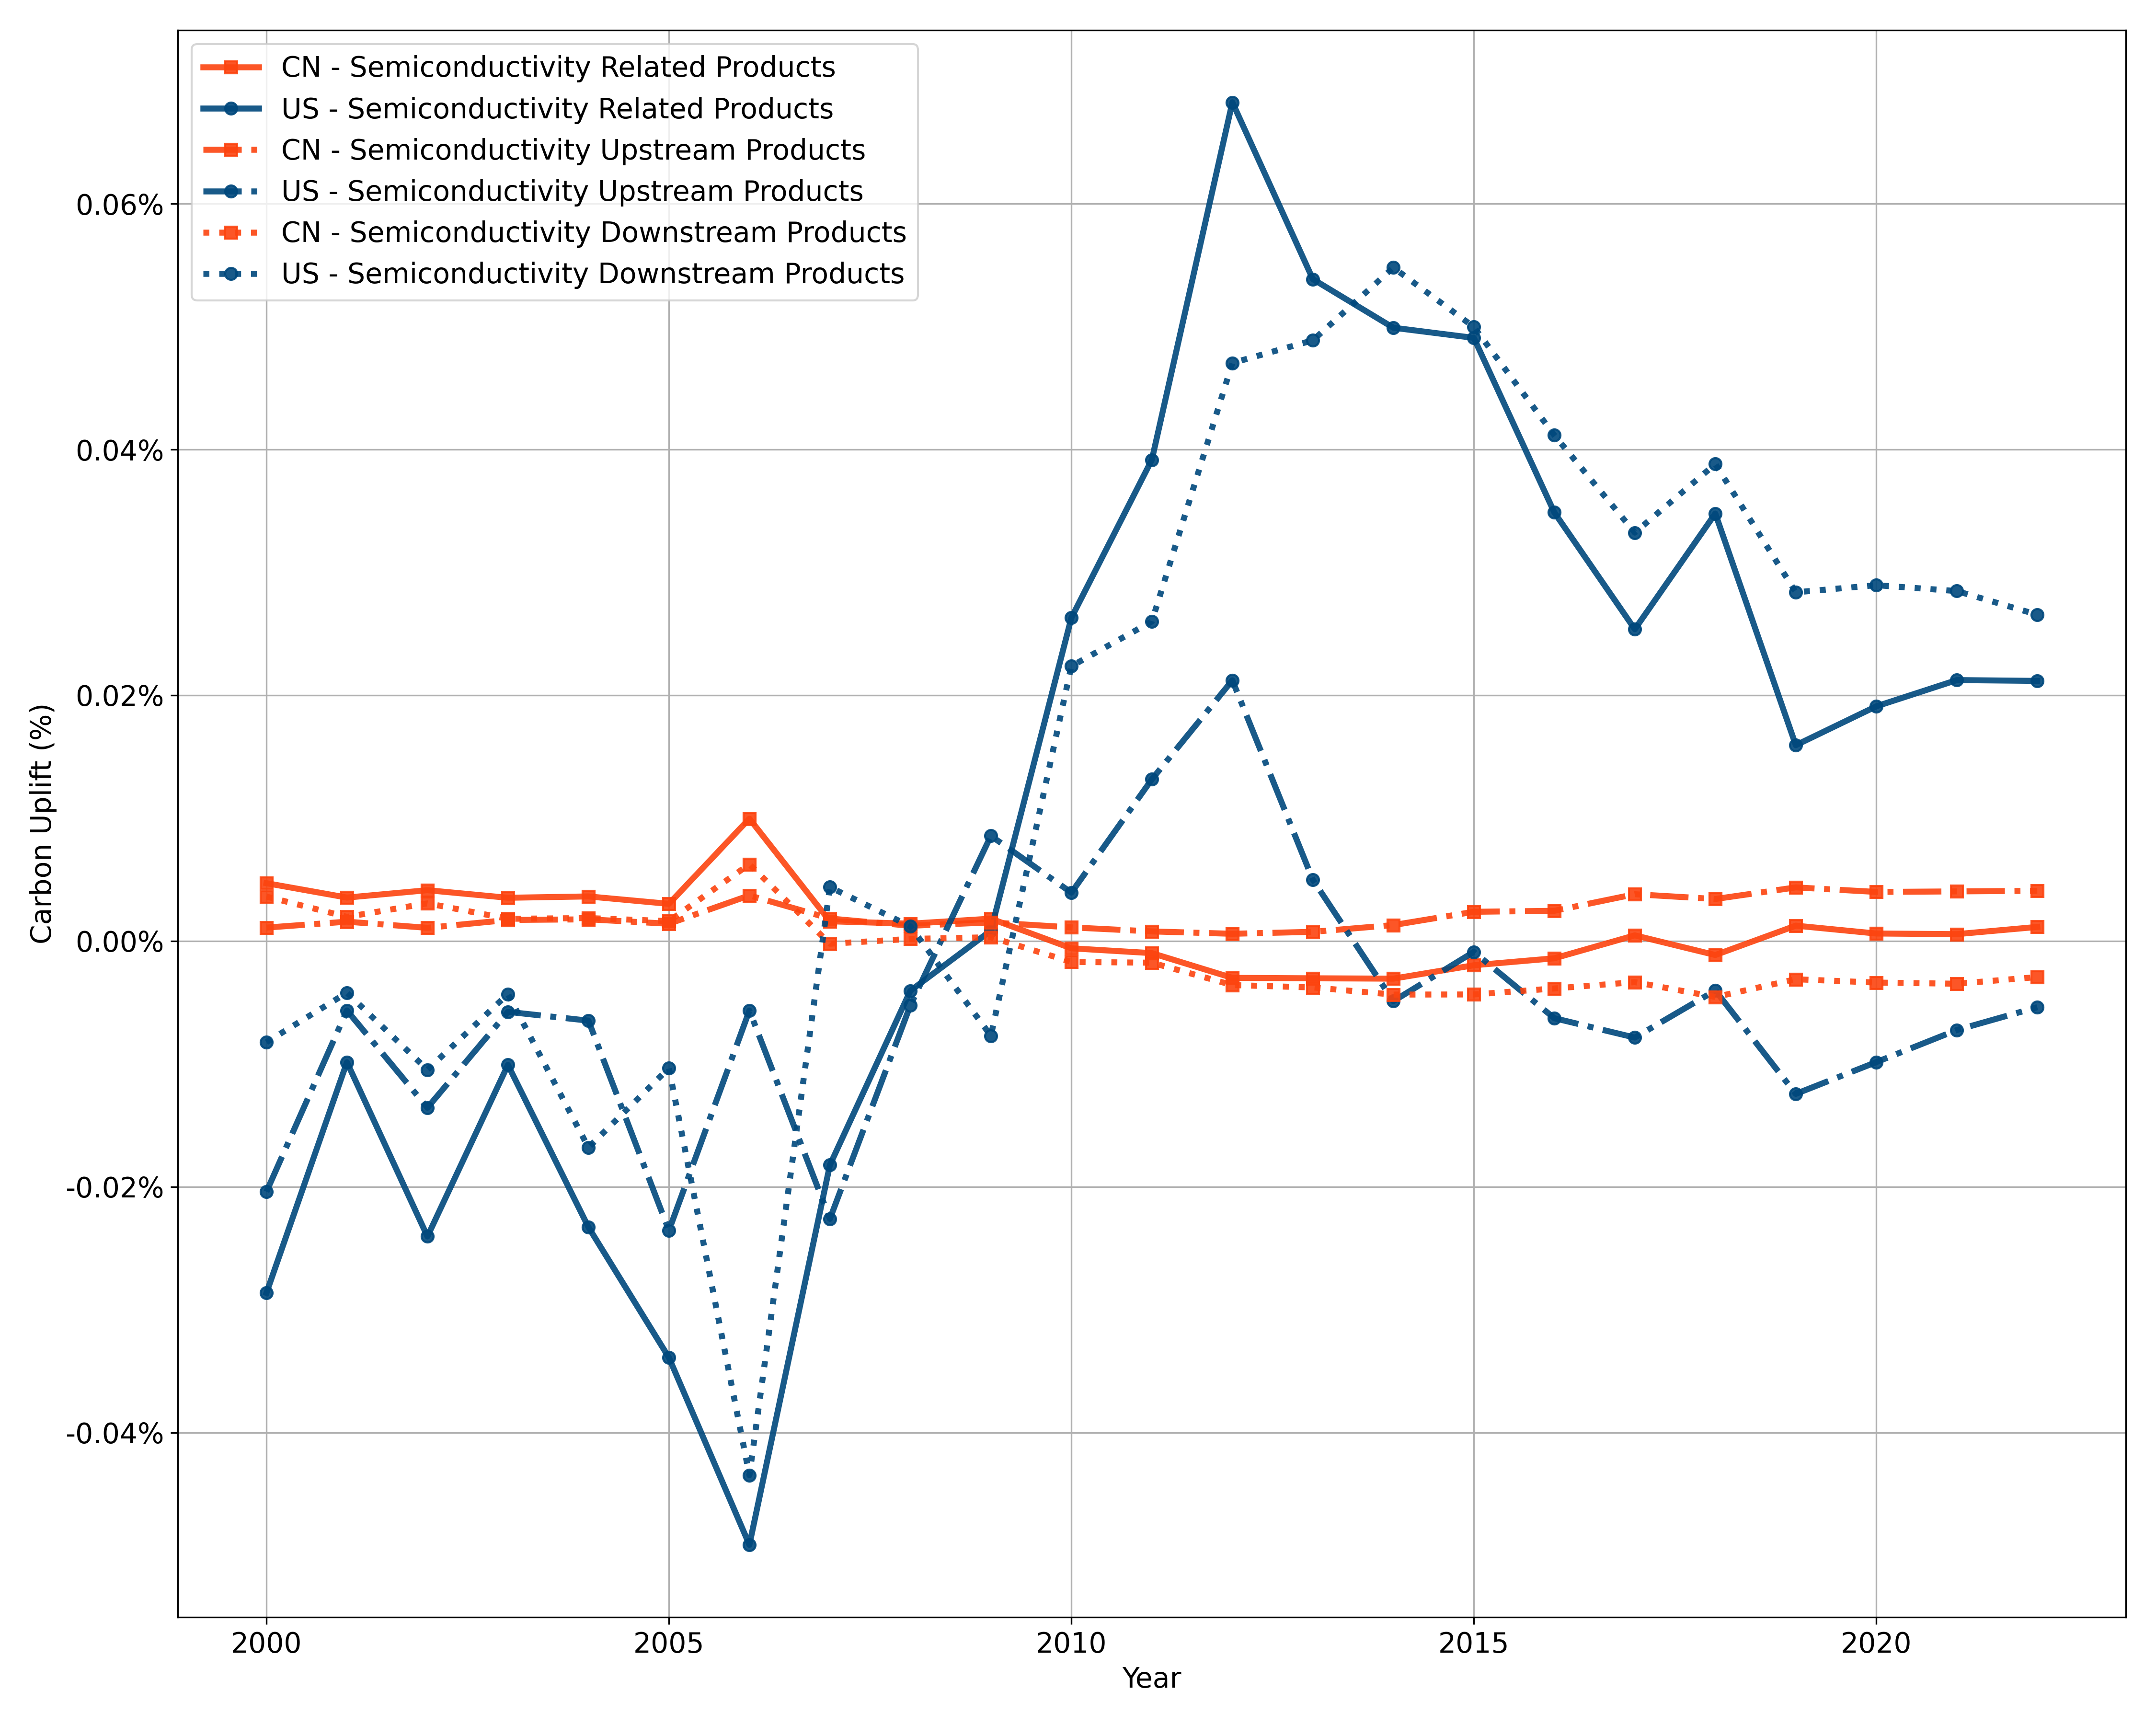
\includegraphics[width=1\textwidth]{figures/Graph/Carbon Uplift Trends If No Sino-US Trade(2000-2022).png}}
 \caption{Carbon Uplift Trends If No Sino-US Trade(2000-2022)}\label{fig:Carbon Uplift Trends If No Sino-US Trade(2000-2022)}
\end{figure}
\fi
\subsection{Carbon Uplift in No Sino-US Semi-conductor Related Products Trade with Gaming Scenario}

The analysis of carbon uplift in three distinct trade scenarios in 2022—absence of all trade, absence of Sino-U.S. trade, and a game theory-based reallocation of trade following a Sino-U.S. trade halt—reveals nuanced effects on carbon emissions on a global scale and across key nations, namely China and the United States, as shown in Figure \ref{fig:Comparison of Carbon Uplift between 3 Scenario}.

In the global context, the elimination of all trade induces a carbon uplift of 0.9106\% for semiconductivity-related products, indicating an increased global carbon footprint due to the localization of production. When bilateral trade between China and the U.S. ceases, the uplift is marginal at 0.0031\%, suggesting that while significant, the carbon footprint impact is not as substantial as one might presume given the volume of trade between these two economies.

The third scenario presents a game-theoretical distribution of trade voids left by halted Sino-U.S. trade, adjusted according to existing production structures and the proportional value output within industry supply chains. Here, a notable shift occurs: the global carbon uplift for related products pivots to 0.3568\%, a figure more pronounced than the no bilateral trade scenario but still less than the no trade scenario. This shift can be attributed to the strategic redistribution of production to regions that may not match the carbon efficiency of the previous Sino-U.S. configuration.

China's unique position as both a massive producer and consumer plays a pivotal role in these scenarios. Under game-theoretic reallocation, China experiences an increase in carbon uplift for related products to 1.2301\%, suggesting that the reallocation may lead to less carbon-efficient production processes taking over the supply void. Conversely, the U.S. sees an uplift of 0.7731\% for related products, hinting at potential increases in carbon emissions due to adjusted trade patterns and possibly less efficient domestic production filling the gap.
\ifincludefigures
\begin{figure}
  \centering
  \makebox[\textwidth][c]{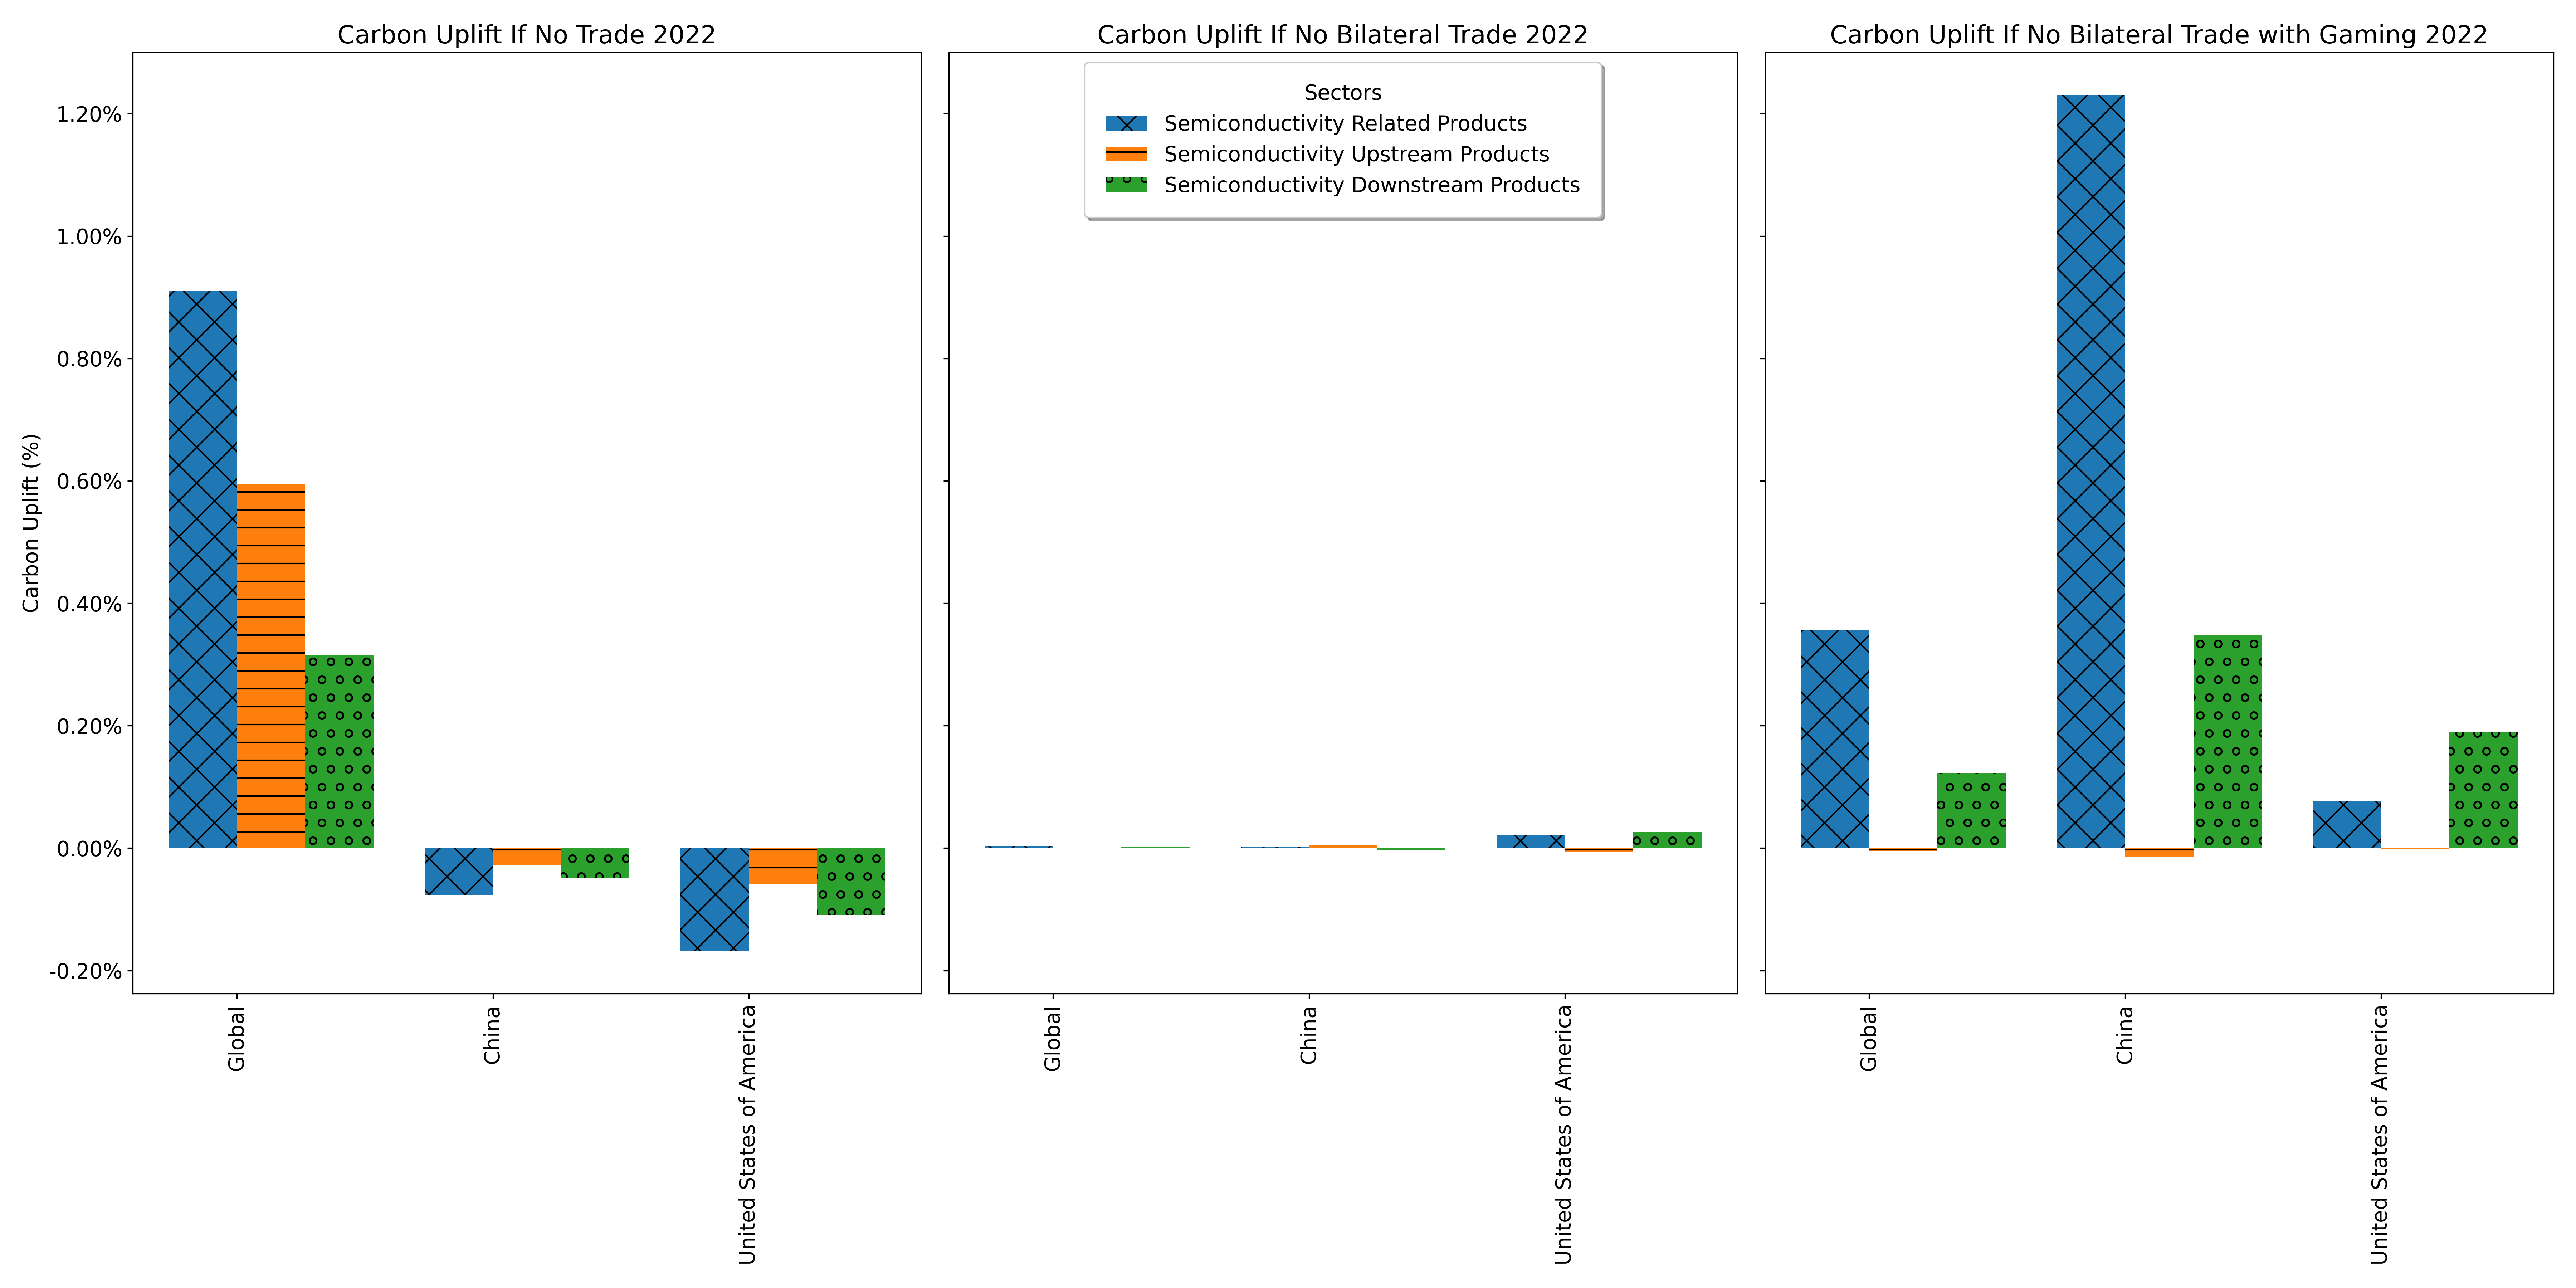
\includegraphics[width=1\textwidth]{figures/Graph/Comparison of Carbon Uplift between 3 Scenario.png}}
  \caption{Comparison of Carbon Uplift between 3 Scenario}\label{fig:Comparison of Carbon Uplift between 3 Scenario}
 \end{figure}
\fi
 In the scenario framed by game theory distribution Figure \ref{fig:Carbon Uplift Trends If No Sino-US with Gaming Trade(2000-2022)}, the strategic reallocation of trade shares between the United States and China shows an upward trajectory in carbon uplift over the years. This model, which diverges from a simplified binary trade or no-trade paradigm Figure \ref{fig:Carbon Uplift Trends If No Sino-US Trade(2000-2022)}, suggests a more complex interaction within the global supply chain, where the interdependence of international trade plays a crucial role.

 The analysis reveals that the carbon uplift in the gaming scenario substantially exceeds the uplift in the simple scenario of domestic production replacing imports. This outcome challenges the notion that ceasing Sino-US trade would lead to a straightforward transition to domestic production for either country. Moreover, the fact that the uplifts are more pronounced under the gaming scenario may imply that the simplified scenario fails to capture the dynamic efficiencies and the clean production structures already present in the Chinese and American industries, which are among the most carbon-efficient on the global stage.
 
 A closer look at the data from 2000 to 2022 reflects this trend. For instance, in the year 2022, China's carbon uplift for semiconductor-related products under the gaming scenario was 1.2301\%, marking a stark contrast to a more modest uplift in the no-trade scenario. Similarly, the United States also exhibited an uplift in the gaming scenario, with figures like 0.7731\% for the year 2022 for semiconductor downstream products. These specific numbers indicate that the advantages of trade in carbon efficiency are not fully realized when trade is simply redistributed without considering the underlying economic and environmental efficiencies.
 
 The larger carbon uplifts observed in this game theory-informed scenario suggest that a hypothetical redistribution of trade shares may lead to less optimal environmental outcomes than the current state of trade. It underscores the potential misalignment between economic strategies and environmental goals, highlighting the importance of considering the full spectrum of supply chain dynamics when assessing the environmental impacts of trade policies.
 \ifincludefigures
 \begin{figure}
  \centering
  \makebox[\textwidth][c]{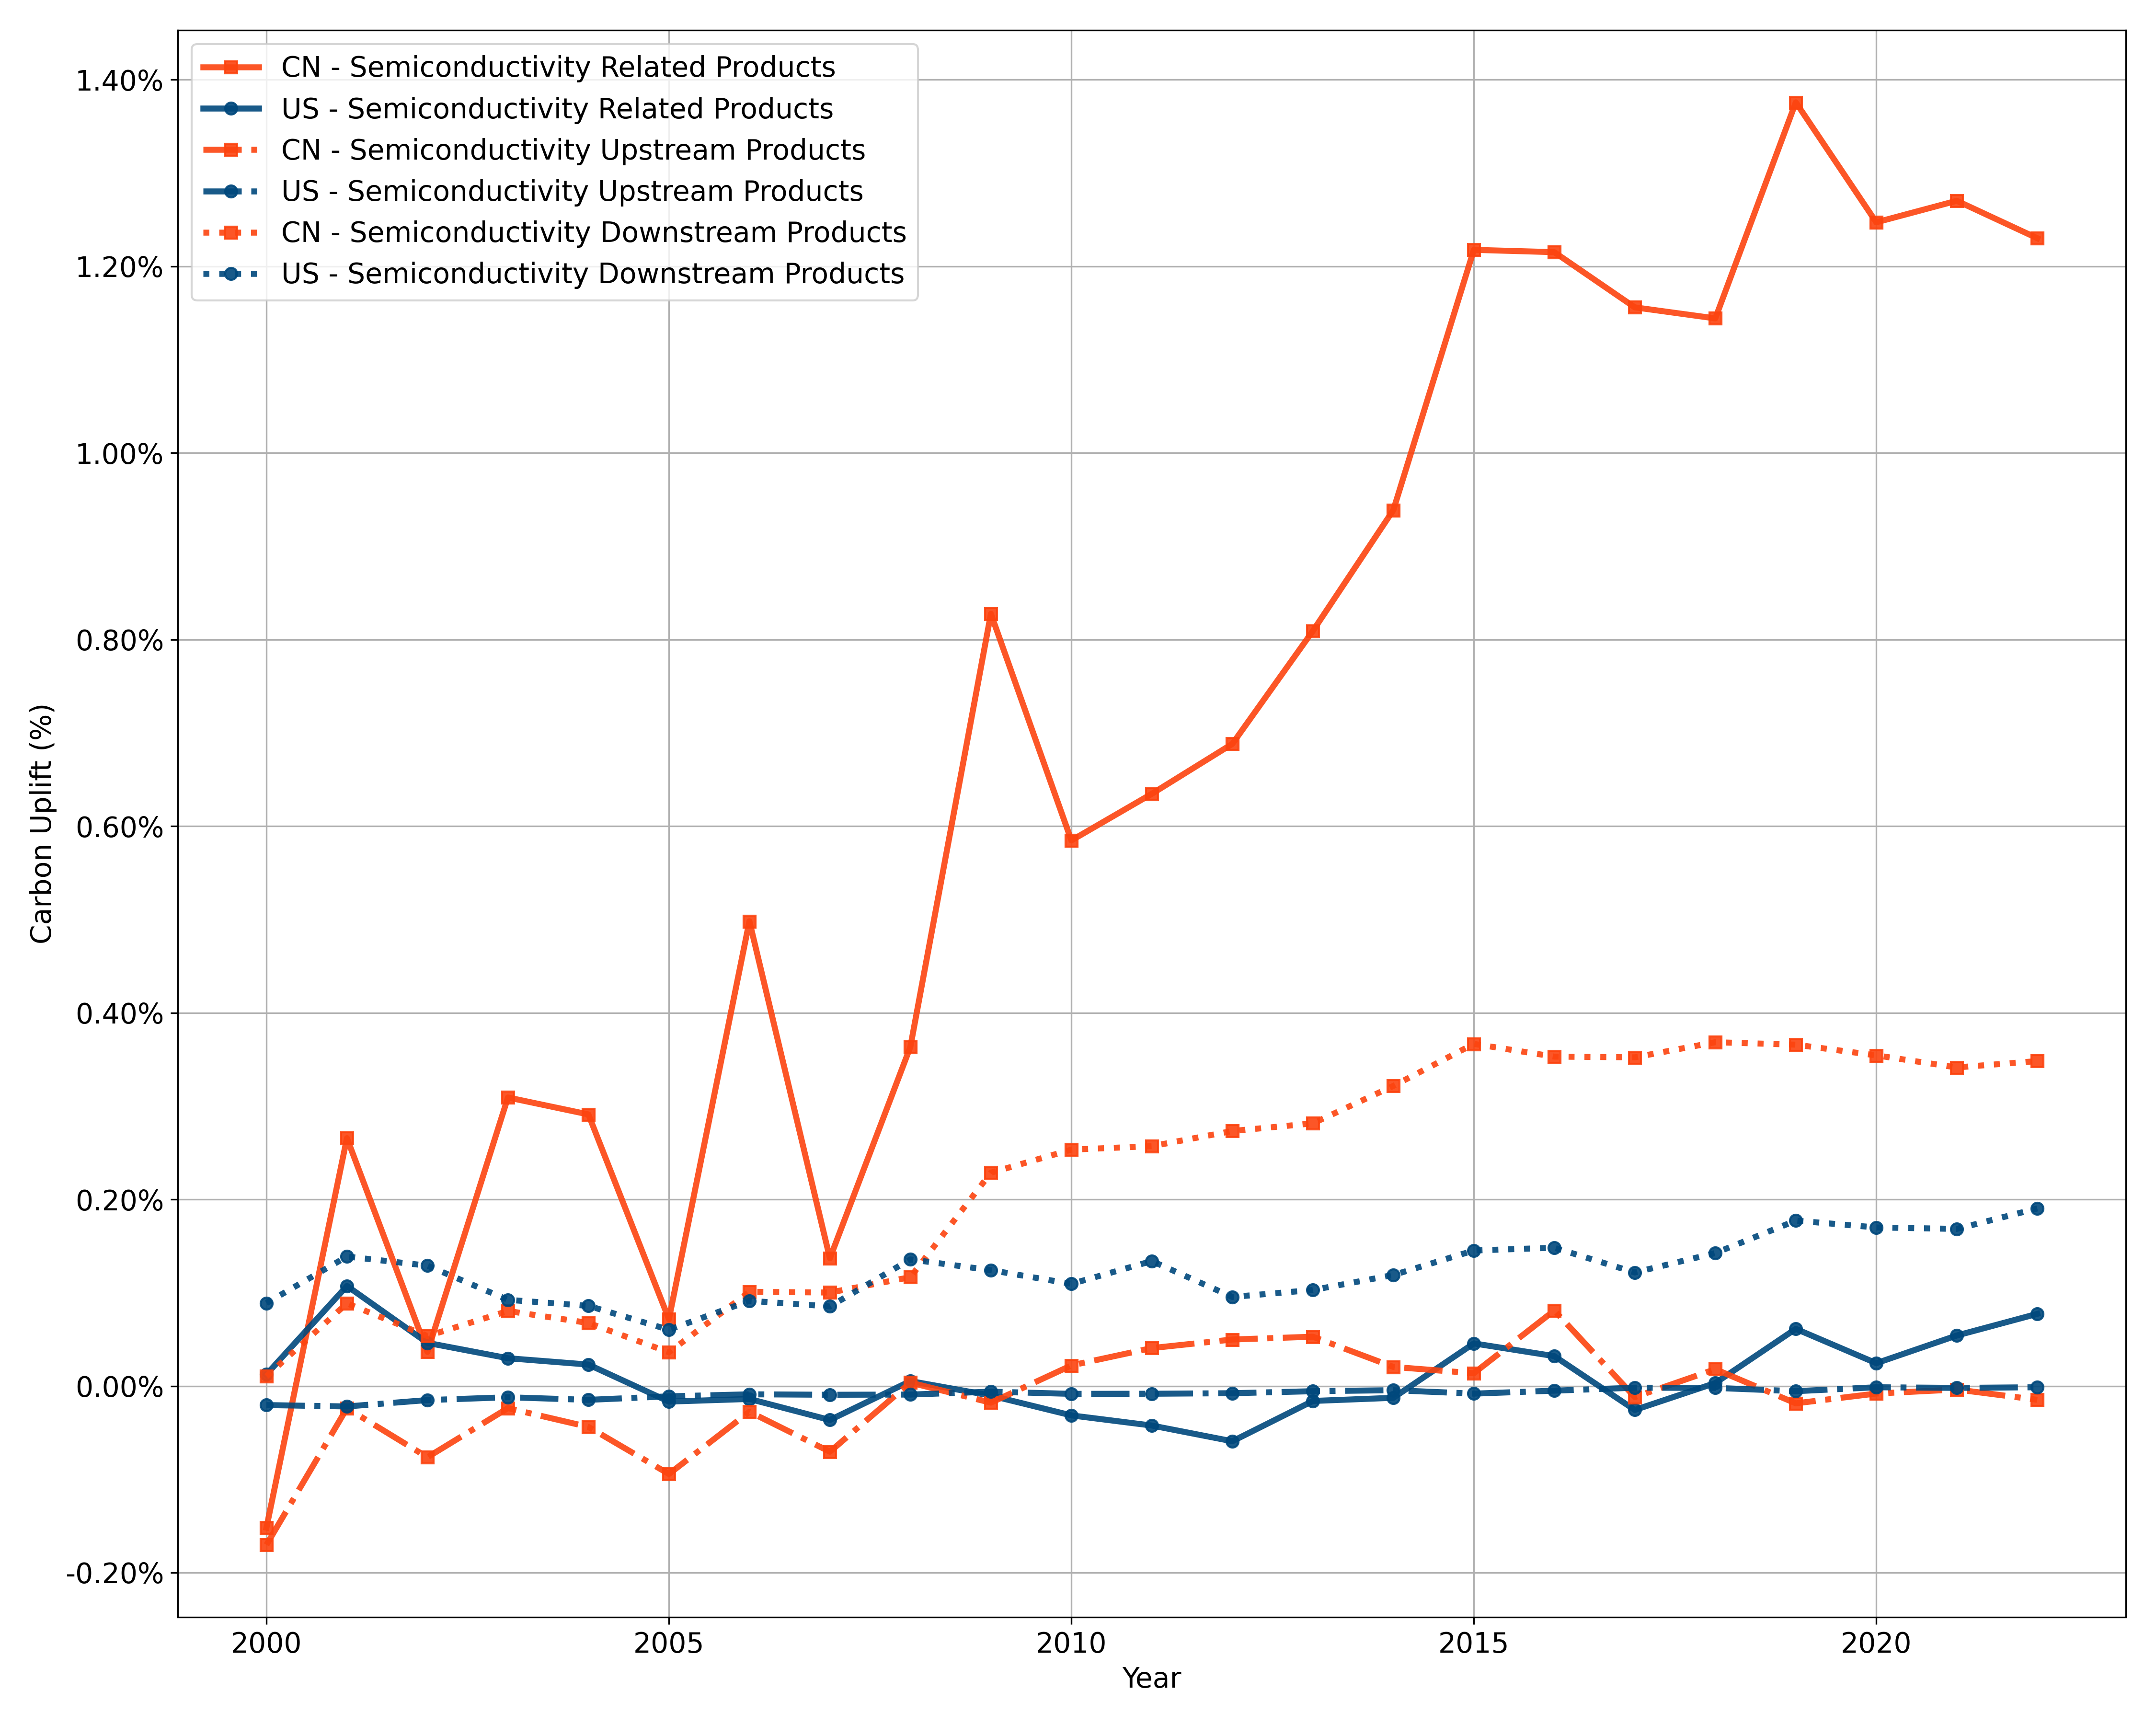
\includegraphics[width=1\textwidth]{figures/Graph/Carbon Uplift Trends If No Sino-US with Gaming Trade(2000-2022).png}}
  \caption{Carbon Uplift Trends If No Sino-US with Gaming Trade(2000-2022)}\label{fig:Carbon Uplift Trends If No Sino-US with Gaming Trade(2000-2022)}
 \end{figure}
\fi
% \subsection{Net Semi-Conductor Export Ratio vs. Carbon Uplift If No Sino-US Trade with Gaming}

% \begin{figure}
%   \centering
%   \makebox[\textwidth][c]{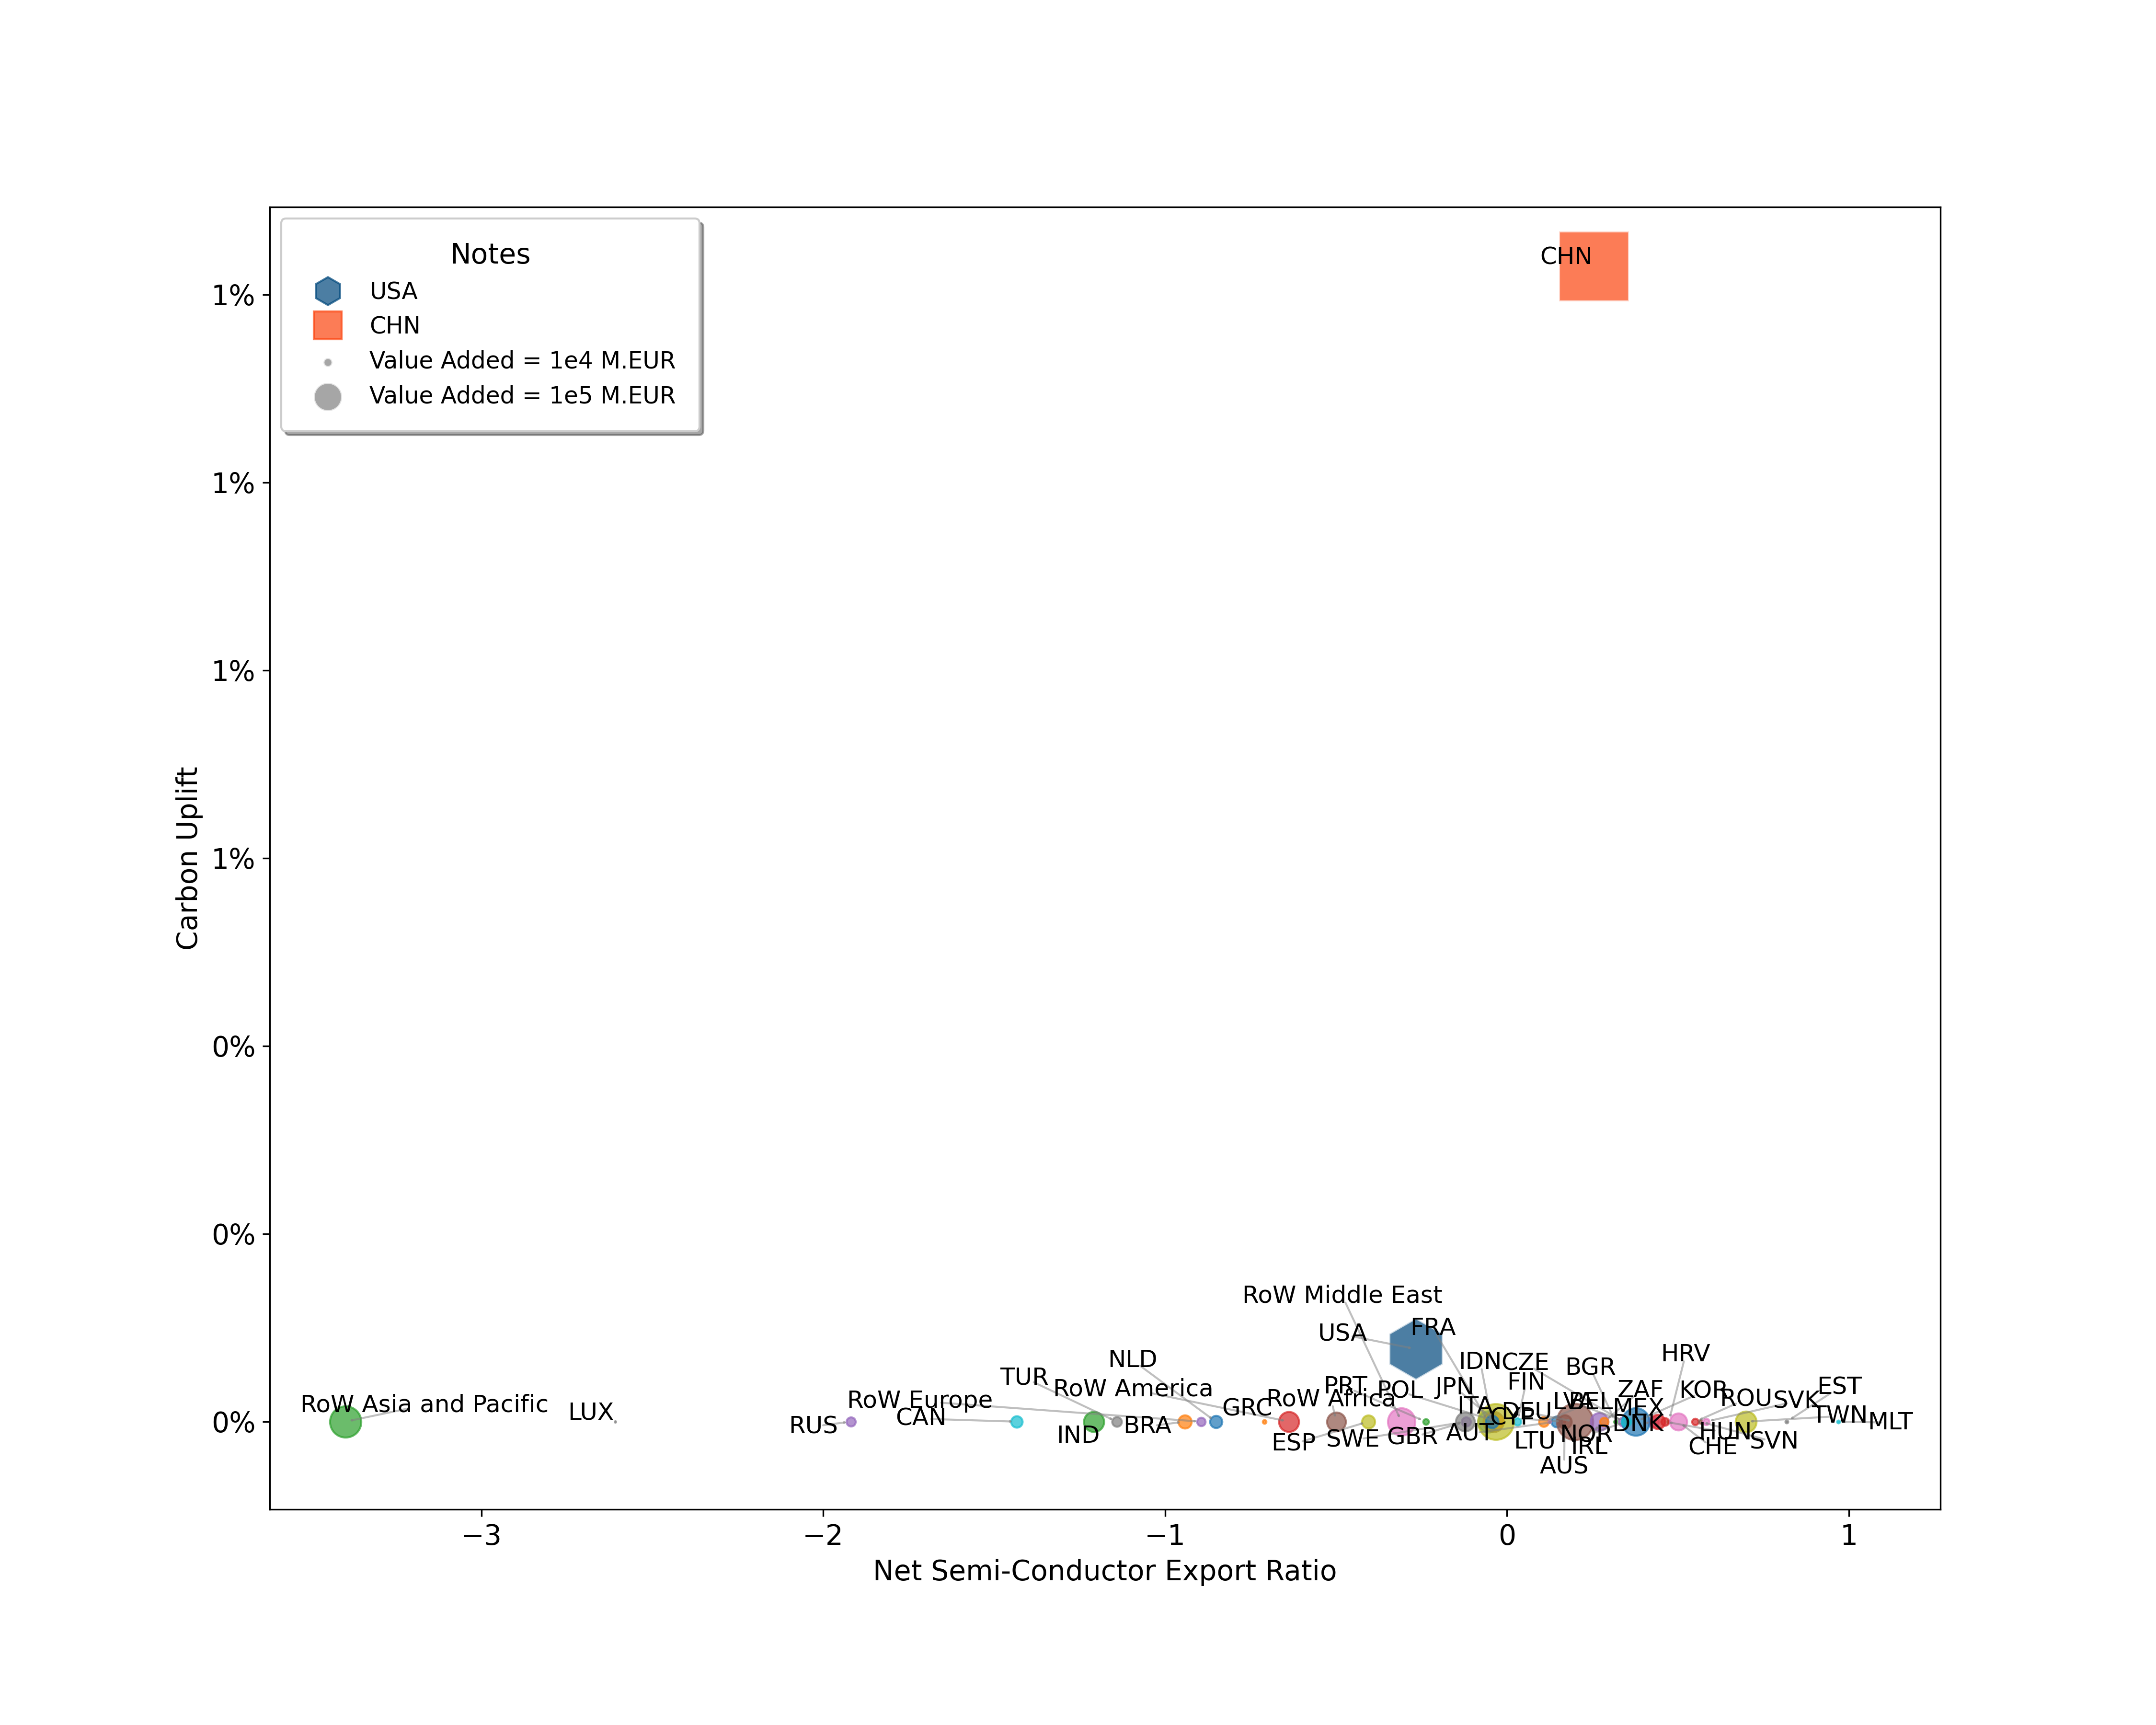
\includegraphics[width=1\textwidth]{figures/Graph/Net Semi-Conductor Export Ratio vs. Carbon Uplift If No Sino-US Trade with Gaming.png}}
%   \caption{Net Semi-Conductor Export Ratio vs. Carbon Uplift If No Sino-US Trade with Gaming}\label{fig:Net Semi-Conductor Export Ratio vs. Carbon Uplift If No Sino-US Trade with Gaming}
%  \end{figure}


\section{Comparison of Global Carbon Stressors}
\subsection{Rank of Carbon Stressors in 2022}
In the scholarly discourse examining the semiconductor industry's carbon footprint, we center upon the segmentation of upstream and downstream sectors. Figure \ref{fig:Rank of Carbon Stressor Heatmap in 2022} provides a granular perspective on the environmental costs of semiconductor production.

For the upstream segments, ``Other non-ferrous metal ores and concentrates'' denote significant carbon stressors, with China presenting approximately 221,397 kg CO2 per M EUR, juxtaposed against the United States`` higher output of around 360,391 kg CO2 per M EUR. In the arena of ''Precious metals" another upstream category, China again indicates a robust emission figure of roughly 304,336 kg CO2 per M EUR, while the United States showcases a lower, yet substantial, figure of approximately 75,648 kg CO2 per M EUR.

Transitioning to the downstream analysis, we observe in the sector ``Electrical machinery and apparatus n.e.c. (31)'' China's carbon stressor is noted at about 10,232 kg CO2 per M EUR, in contrast to the United States' figure of around 18,798 kg CO2 per M EUR. In the domain of ``Office machinery and computers (30)'' the carbon emission intensity for China is captured at nearly 9,244 kg CO2 per M EUR, with the United States reflecting a higher emission intensity of approximately 18,205 kg CO2 per M EUR. Moreover, within ``Radio, television and communication equipment and apparatus (32)'' China's carbon stressor stands at around 25,205 kg CO2 per M EUR, with the United States slightly elevated at 22,833 kg CO2 per M EUR. Lastly, in the ``Medical, precision and optical instruments, watches and clocks (33)'' sector, the data delineate China at roughly 5,285 kg CO2 per M EUR and the United States at about 22,749 kg CO2 per M EUR.

The visualization method adopted in the paper, the ``Rank of Carbon Stressor Heatmap in 2022'' is predicated upon a ranking-based depiction rather than raw numerical values. This analytical choice is made to circumvent the limitations posed by the disparate magnitude of raw data, ensuring a more coherent and comparative visual comprehension of the carbon stressors across various sectors and countries.
\ifincludefigures 
\begin{figure}
 \centering
 \makebox[\textwidth][c]{\includegraphics[width=1\textwidth]{figures/Graph/Rank of Carbon Stressor Heatmap in 2022.png}}
 \caption{Rank of Carbon Stressors Heat Map in 2022}\label{fig:Rank of Carbon Stressor Heatmap in 2022}
\end{figure}
\fi
\subsection{Carbon Stressor Trends (2000-2022)}
The intricate graph Figure \ref{fig:Carbon Stressor Trends (2000-2022)} delineates the carbon stressor in kilograms of CO2 equivalent per million EUR of product value (kg CO2 eq./M EUR) for China, the United States, and globally, across all products and within the semiconductor sector, including both its upstream and downstream components.

Beginning the analysis with the year 2000, China's carbon stressor in the semiconductor industry's related products was 140,031 kg CO2 eq./M EUR, which, when compared to the upstream and downstream sectors—1,466,154 and 63,334 kg CO2 eq./M EUR, respectively—indicates a significant carbon efficiency in the production of specific semiconductor-related outputs. Over the subsequent years, a downward trend is evident, with fluctuations that suggest adjustments and improvements in production efficiency, concluding with the 2022 figures of 24,511 kg CO2 eq./M EUR for related products, and 141,159 kg CO2 eq./M EUR for downstream, against an upstream value of 271,619 kg CO2 eq./M EUR.

For the United States, the year 2000 starts with a carbon stressor of 433,602 kg CO2 eq./M EUR for related products, and 372,360 and 405,985 kg CO2 eq./M EUR for the downstream and upstream sectors, respectively. This highlights a greater initial carbon stressor compared to China. Over the years, the US shows a trend of reducing this stressor across all sectors, particularly in the related and downstream products, culminating in 2022 with values of 22,343 and 21,392 kg CO2 eq./M EUR for related and downstream products, and a higher but reduced upstream stressor of 83,254 kg CO2 eq./M EUR.

The global trends mirror this reduction, starting from 71,282 kg CO2 eq./M EUR for related products and 53,260 and 658,171 kg CO2 eq./M EUR for downstream and upstream sectors in 2000, to 46,830 and 35,374 kg CO2 eq./M EUR for related and downstream products, and 344,678 kg CO2 eq./M EUR for upstream products in 2022. The general trend shows a global drive towards higher carbon efficiency, albeit with regional disparities.

The relationship between these carbon stressors and the previously discussed carbon uplift in a no-trade scenario is telling. The carbon stressor is a measure of the efficiency of production—a lower figure suggests a higher carbon efficiency. In the absence of trade, especially between China and the US, we see the carbon uplift—representing an increase in carbon emissions—reducing over time, which could imply that the efficiency of local production is increasing, thus lessening the potential negative environmental impacts of trade disruptions. This supports the initial analysis that suggests that the semiconductor industry, particularly in China and the US, is advancing towards greater carbon efficiency. Despite this progress, the complexities of global trade and production processes indicate that continuous improvements and collaborations are necessary to further mitigate the carbon footprint of this vital sector.
\ifincludefigures
\begin{figure}
 \centering
 \makebox[\textwidth][c]{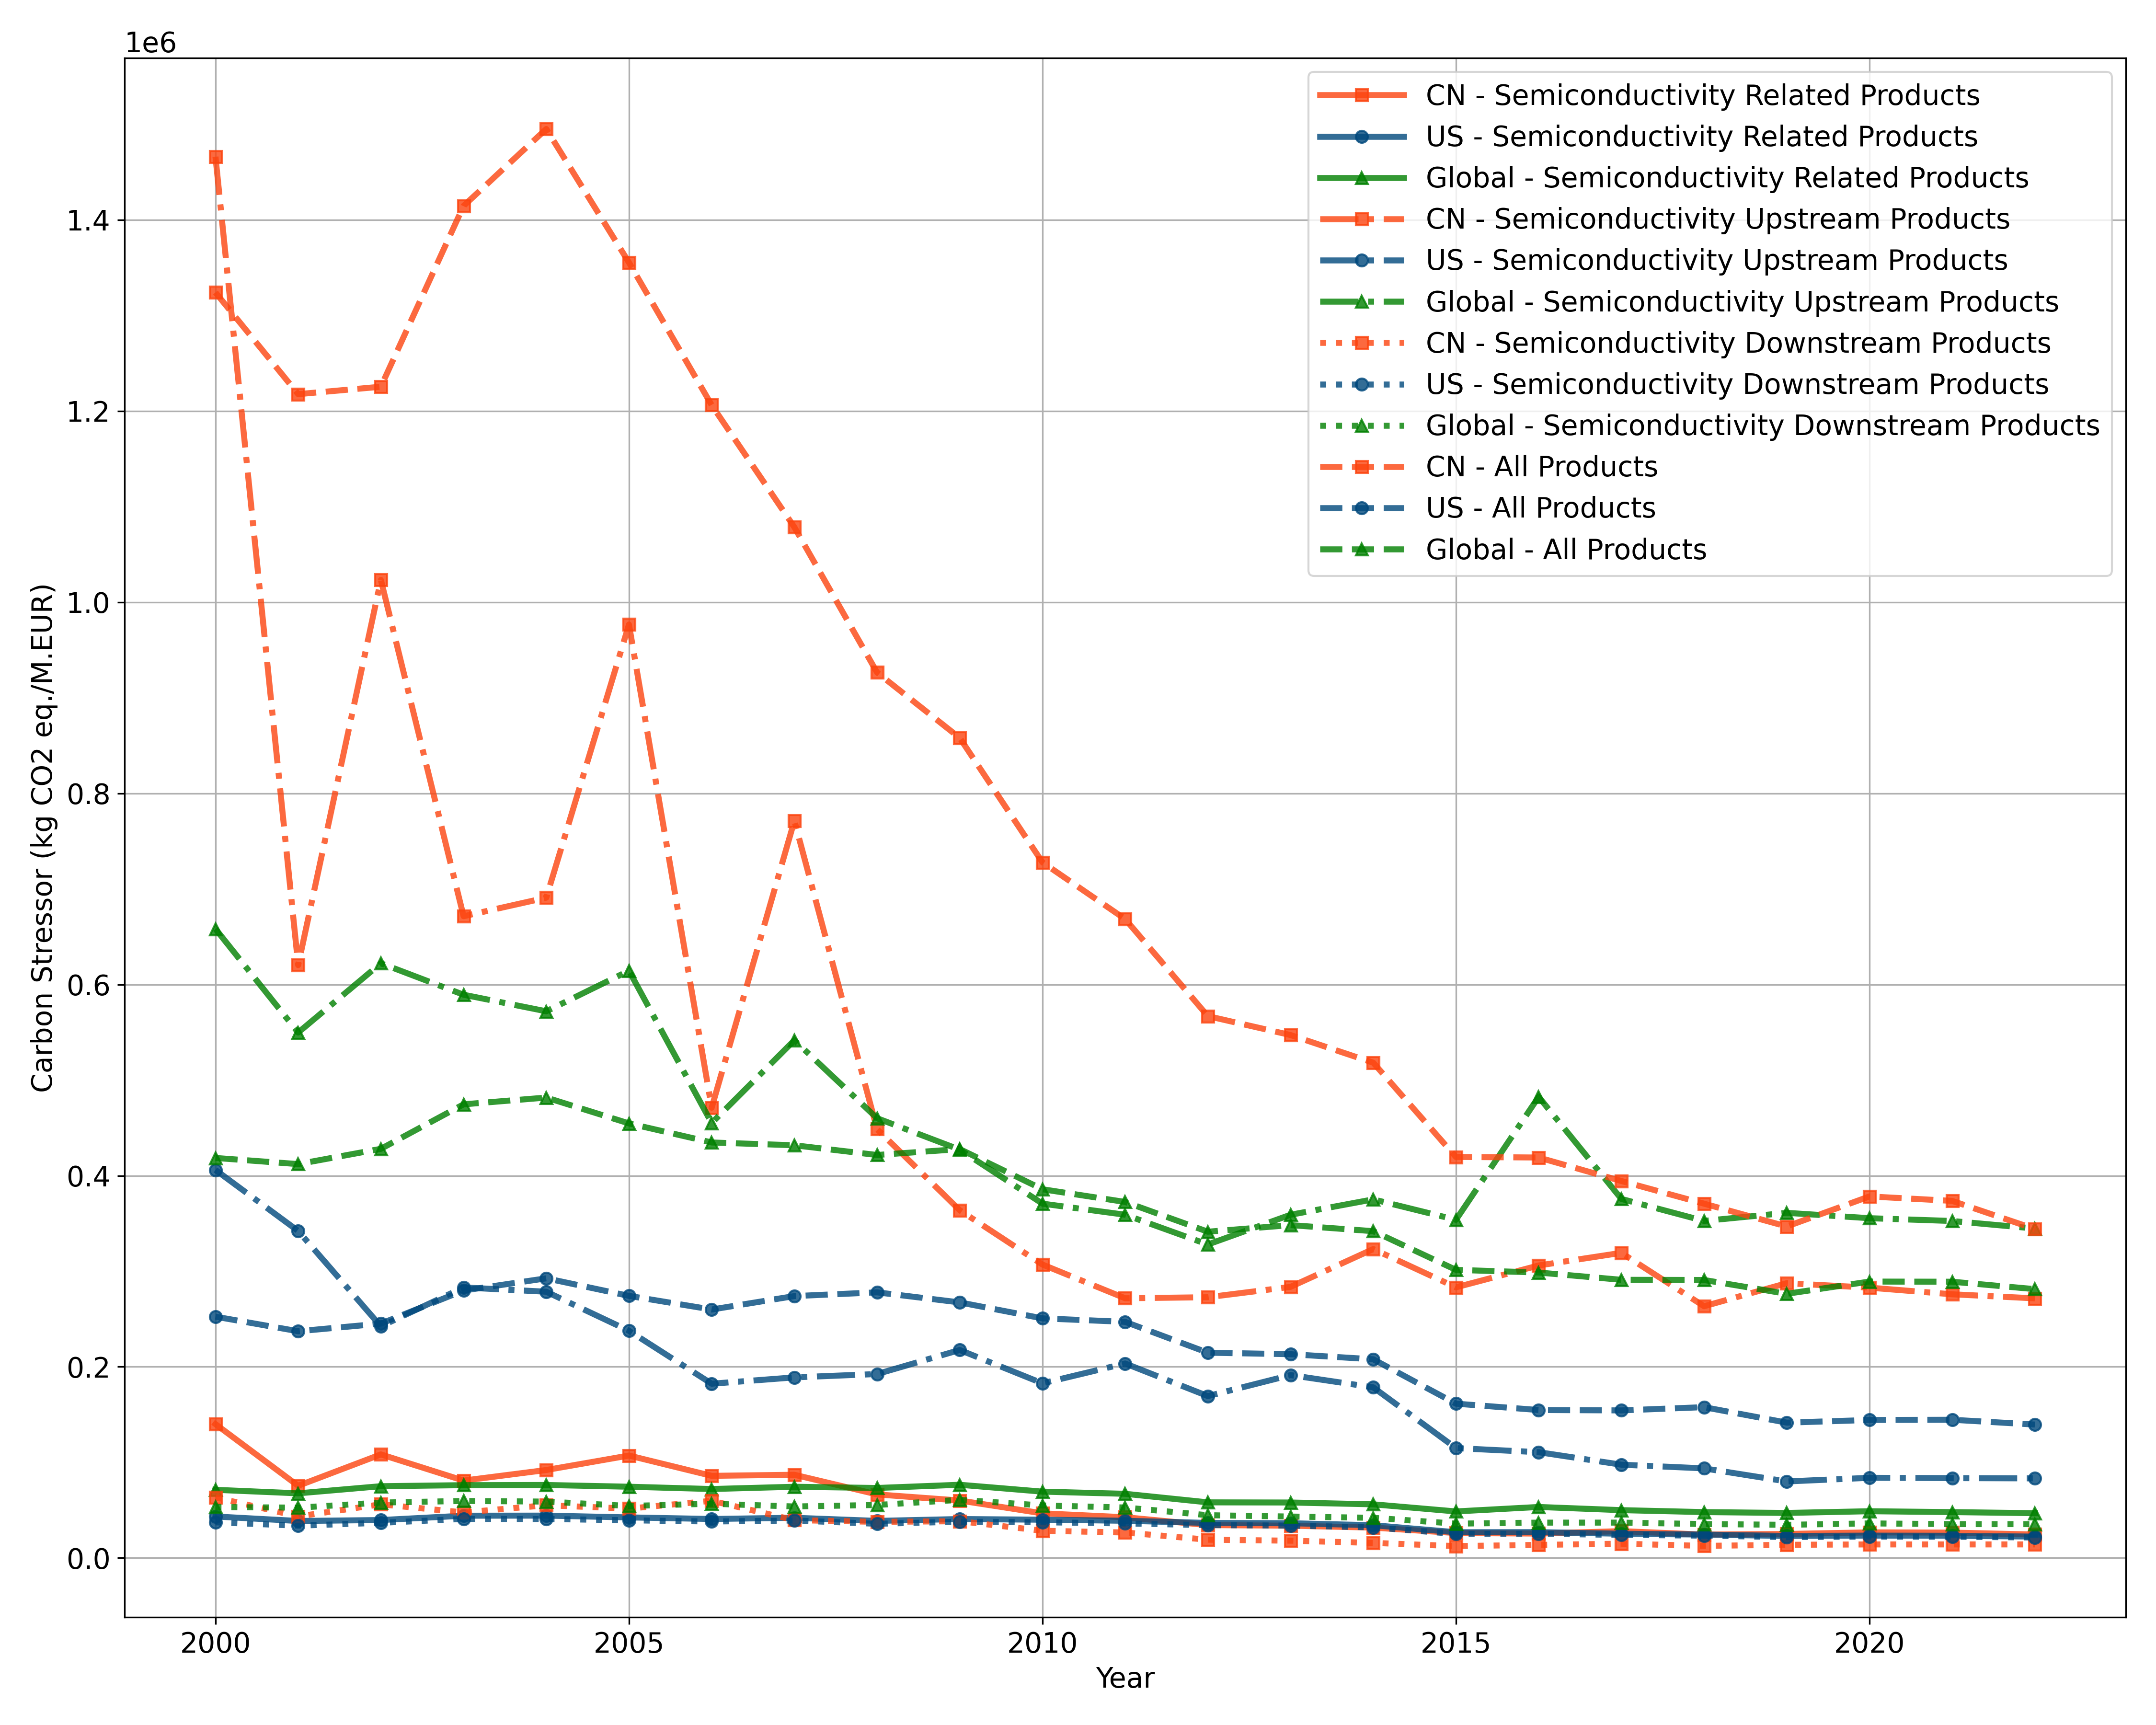
\includegraphics[width=1\textwidth]{figures/Graph/Carbon Stressor Trends (2000-2022).png}}
 \caption{Carbon Stressors Trends (2000-2022)}\label{fig:Carbon Stressor Trends (2000-2022)}
\end{figure}
\fi
\subsection{Carbon Stressor in Different Sectors 2022}
Figure \ref{fig:Carbon Stressor in Different Sectors 2022} reveals the heterogeneous nature of the carbon stressor across regions and sectors, underscoring the complex interdependencies and varied stages of development. The metric, measured in kilograms of CO2 equivalent per product value, illuminates the environmental cost of economic activities. 

Africa's substantial carbon stressor figures (approx. 249,685 kg CO2 eq./M EUR for related products) hint at the potential for improvement in production efficiencies or the necessity for technology transfer to reduce the environmental impact of its burgeoning semiconductor industry.

Focusing on the Americas, the data depicts a relatively low carbon stressor in the related products sector at approximately 27,254 kg CO2 eq./M EUR, which, juxtaposed with the significant figure in the upstream sector (approx. 178,097 kg CO2 eq./M EUR), indicates a remarkable discrepancy between the different stages of semiconductor production.

China (CHN), a key player in this narrative, shows a carbon stressor of approximately 24,511 kg CO2 eq./M EUR for related products and 141,159 kg CO2 eq./M EUR for downstream products. These figures, when aligned with its upstream carbon stressor of about 271,619 kg CO2 eq./M EUR, suggest a more efficient downstream production relative to the upstream processes.

When we consider the United States (USA), the carbon stressor in related semiconductor products is approximately 22,343 kg CO2 eq./M EUR, with the upstream value at 83,254 kg CO2 eq./M EUR, and downstream at about 21,392 kg CO2 eq./M EUR. This denotes a more balanced carbon stressor across the sectors compared to other regions, reflecting perhaps a more mature market with optimized production processes.

The global view encapsulates these variances, with a general carbon stressor in semiconductor-related products at approximately 46,830 kg CO2 eq./M EUR, indicating the worldwide impact of this industry. This serves as a critical indicator for policymakers and industry leaders to assess and strategize for a sustainable progression of the semiconductor industry.
\ifincludefigures
\begin{figure}
 \centering
 \makebox[\textwidth][c]{\includegraphics[width=1\textwidth]{figures/Graph/Carbon Stressor in Different Sectors 2022.png}}
 \caption{Carbon Stressors in Different Sectors 2022}\label{fig:Carbon Stressor in Different Sectors 2022}
\end{figure}
\fi

%%==================================================
%% conclusion.tex for BIT Master Thesis
%% modified by yang yating
%% version: 0.1
%% last update: Dec 25th, 2016
%%==================================================
\chapter{Conclusions and Policy Recommendations}
\section{Conclusions}


The culmination of this study into the effects of trade protectionism, particularly within the semiconductor industry, underscores the nuanced implications for carbon emissions on a global scale. The analytical results, as shown in Table \ref{tab:SummaryTable}, suggest that the current Sino-US trade, under the prevailing global production framework, contributes substantially to the reduction of global carbon footprint, an insight previously obscured by simplistic substitution methodologies.

The data reveals that the global carbon uplift percentage, which signifies the increase in the carbon footprint under the modelled scenarios, paints a telling picture of the benefits of current trade patterns. For instance, the no-trade carbon uplift globally for semiconductor-related products was marked at 0.9106\%, while the no Sino-US trade with gaming scenario exhibited a significantly higher uplift of 0.3568\% in China and 1.2301\% in the United States, signifying the substantial carbon mitigation benefits accrued through the current trade relations. This is contrasted with a global uplift of merely 0.0031\% under the no Sino-US trade scenario, which does not account for the more complex and realistic inter-country competitive dynamics.

Similarly, for upstream and downstream semiconductor products, the no-trade scenario indicates potential global uplifts of 0.5955\% and 0.3152\%, respectively. However, when incorporating a gaming trade redistribution approach, the results showcase an intriguing shift with a carbon uplift of -0.0043\% globally for upstream products, and a more pronounced uplift for downstream products at 0.1229\%. These variations underscore the intricate interplay between trade policies and environmental outcomes.

In conclusion, our comprehensive and granular approach to modeling trade restrictions and their impact on carbon emissions provides a more accurate representation of the potential environmental repercussions. The data-driven insights confirm that trade between China and the United States has been a key driver in mitigating carbon emissions, challenging the notion that protectionism could be a boon for environmental sustainability. As we navigate the complexities of global trade and its environmental impact, it becomes increasingly evident that collaboration, rather than protectionism, is pivotal in fostering a global reduction in carbon emissions.







\begin{table}
    \centering
    \caption{Summary of Carbon Uplift and Stressor Data for Semiconductivity Products}
    \label{tab:SummaryTable}
    \begin{tabular}{lccc}
    \hline
    \textbf{Products} & \textbf{Global} & \textbf{China} & \textbf{United States} \\
    \hline
    \multicolumn{4}{l}{\textit{Semiconductivity Related Products}} \\
    No Trade Carbon Uplift & 0.9106\% & -0.0768\% & -0.1678\% \\
    No Sino-US Trade Carbon Uplift & 0.0031\% & 0.0011\% & 0.0212\% \\
    No Sino-US Trade with Gaming Uplift & 0.3568\% & 1.2301\% & 0.0773\% \\
    Carbon Stressor (kg CO$_2$ eq./M.EUR) & 46,830.10 & 24,511.12 & 22,343.31 \\
    Net Export Rate & 0.0000\% & 25.4251\% & -26.6277\% \\
    \hline
    \multicolumn{4}{l}{\textit{Semiconductivity Upstream Products}} \\
    No Trade Carbon Uplift & 0.5955\% & -0.0280\% & -0.0590\% \\
    No Sino-US Trade Carbon Uplift & 0.0004\% & 0.0041\% & -0.0054\% \\
    No Sino-US Trade with Gaming Uplift & -0.0043\% & -0.0148\% & -0.0013\% \\
    Carbon Stressor (kg CO$_2$ eq./M.EUR) & 344,677.88 & 271,619.23 & 83,254.16 \\
    Net Export Rate & 0.0000\% & 21.3270\% & 65.2615\% \\
    \hline
    \multicolumn{4}{l}{\textit{Semiconductivity Downstream Products}} \\
    No Trade Carbon Uplift & 0.3152\% & -0.0488\% & -0.1088\% \\
    No Sino-US Trade Carbon Uplift & 0.0026\% & -0.0029\% & 0.0266\% \\
    No Sino-US Trade with Gaming Uplift & 0.1229\% & 0.3482\% & 0.1903\% \\
    Carbon Stressor (kg CO$_2$ eq./M.EUR) & 35,373.63 & 14,159.19 & 21,392.43 \\
    Net Export Rate & 0.0000\% & 25.5608\% & -27.0224\% \\
    \hline
    \end{tabular}
\end{table}

\section{Policy Recommendations}
The insights garnered from this study provide a pivotal foundation for formulating informed policy recommendations aimed at optimizing trade practices to enhance global environmental outcomes, particularly within the semiconductor industry. The evidence suggests that the interplay between international trade and carbon emissions is intricate and highly impactful. Therefore, it is essential for policy frameworks to leverage this relationship to foster a reduction in global carbon emissions through strategic trade agreements and regulations.

Firstly, the findings advocate for the continuation and enhancement of collaborative trade agreements, especially between major economies such as the United States and China. These partnerships have proven to be crucial in mitigating the carbon footprint associated with the semiconductor industry. Policies that encourage open trade, while also integrating strict environmental standards, can serve to both sustain economic growth and enhance environmental outcomes. Governments should consider trade policies that incentivize industries to adopt cleaner technologies and more efficient production methods. This could be achieved through tariff reductions on environmentally friendly goods and technologies, or through penalties for the trade of goods produced with high carbon footprints.

Secondly, the significance of technology transfer agreements in reducing global carbon emissions cannot be overstated. Developed countries, which often have access to more advanced technologies, should be encouraged to facilitate technology transfer to developing countries. This would not only help in leveling the playing field but also in reducing the global carbon emissions by enabling these countries to leapfrog to cleaner technologies. Such policies could be supported by international bodies and could include financial incentives or support mechanisms that make it easier for developing nations to access these technologies.

Additionally, there is a clear need for more comprehensive and transparent reporting and monitoring of carbon emissions on an international scale. The establishment of a global registry for carbon emissions from trade, which could track emissions from the production and transportation of goods, would enable better enforcement of international agreements and help in setting more targeted and effective carbon reduction goals.

Lastly, considering the complex dynamics revealed through the gaming trade redistribution scenarios, policies should also focus on the strategic distribution of production capabilities globally. Encouraging diversification of production and investment in renewable energy sources across different regions could help reduce the dependency on specific trade routes or production hubs, which often leads to higher emissions. Diversifying production can also help reduce vulnerabilities in the global supply chain, making it more resilient to shocks and stresses, which is increasingly important in a globalized economy.

In conclusion, it is imperative that trade policies are designed with a dual focus on economic growth and environmental sustainability. This research underscores the potential for trade to act as a lever for environmental improvement, provided it is managed and regulated thoughtfully and strategically. By embracing these policy recommendations, governments and international bodies can make significant strides towards achieving a sustainable balance between global trade efficiency and environmental conservation.
% 后置部分
\backmatter

\begin{bibprint}
  \printbibliography[heading=none]
\end{bibprint}
% 结论:在结论相应的 TeX 文件处进行结论部分的撰写
% 参考文献:如无特殊需要,参考文献相应的 TeX 文件无需改动,添加参考文献请使用 BibTeX 的格式
%   添加至 misc/ref.bib 中,并在正文的相应位置使用 \cite{xxx} 的格式引用参考文献
% %%
% The BIThesis Template for Bachelor Graduation Thesis
%
% 北京理工大学毕业设计(论文)参考文献 —— 使用 XeLaTeX 编译
%
% Copyright 2020-2023 BITNP
%
% This work may be distributed and/or modified under the
% conditions of the LaTeX Project Public License, either version 1.3
% of this license or (at your option) any later version.
% The latest version of this license is in
%   http://www.latex-project.org/lppl.txt
% and version 1.3 or later is part of all distributions of LaTeX
% version 2005/12/01 or later.
%
% This work has the LPPL maintenance status `maintained'.
%
% The Current Maintainer of this work is Feng Kaiyu.
%
% Compile with: xelatex -> biber -> xelatex -> xelatex
%
% 如无特殊需要,本页面无需更改

\begin{bibprint}

% -------------------------------- 示例内容(正式使用时请删除) ------------------------------------- %

% 抑制多次调用 \printbibliography 的 warning,只有示例代码会需要此语句。
\BiblatexSplitbibDefernumbersWarningOff

\textcolor{blue}{参考文献书写规范}

\textcolor{blue}{参考国家标准《信息与文献参考文献著录规则》【GB/T 7714—2015】,参考文献书写规范如下:}

\textcolor{blue}{\textbf{1. 文献类型和标识代码}}

\textcolor{blue}{普通图书:M}\qquad\textcolor{blue}{会议录:C}\qquad\textcolor{blue}{汇编:G}\qquad\textcolor{blue}{报纸:N}

\textcolor{blue}{期刊:J}\qquad\textcolor{blue}{学位论文:D}\qquad\textcolor{blue}{报告:R}\qquad\textcolor{blue}{标准:S}

\textcolor{blue}{专利:P}\qquad\textcolor{blue}{数据库:DB}\qquad\textcolor{blue}{计算机程序:CP}\qquad\textcolor{blue}{电子公告:EB}

\textcolor{blue}{档案:A}\qquad\textcolor{blue}{舆图:CM}\qquad\textcolor{blue}{数据集:DS}\qquad\textcolor{blue}{其他:Z}

\textcolor{blue}{\textbf{2. 不同类别文献书写规范要求}}

\textcolor{blue}{\textbf{期刊}}

\noindent\textcolor{blue}{[序号] 主要责任者. 文献题名[J]. 刊名, 出版年份, 卷号(期号): 起止页码. }
\cite{yuFeiJiZongTiDuoXueKeSheJiYouHuaDeXianZhuangYuFaZhanFangXiang2008, Hajela2012Application}

\printbibliography [type=article,heading=none] 

\textcolor{blue}{\textbf{普通图书}}

\noindent\textcolor{blue}{[序号] 主要责任者. 文献题名[M]. 出版地: 出版者, 出版年: 起止页码. }
\cite{张伯伟2002全唐五代诗格会考, OBRIEN1994Aircraft}

\printbibliography [keyword={book},heading=none] 

\textcolor{blue}{\textbf{会议论文集}}

\noindent\textcolor{blue}{[序号] 主要责任者.题名:其他题名信息[C]. 出版地: 出版者, 出版年. }
\cite{雷光春2012}

\printbibliography [type=proceedings,heading=none] 

\textcolor{blue}{\textbf{专著中析出的文献}}

\noindent\textcolor{blue}{[序号] 析出文献主要责任者. 析出题名[M]//专著主要责任者. 专著题名. 出版地: 出版者, 出版年: 起止页码. }
\cite{白书农}

\printbibliography [type=inbook,heading=none] 

\textcolor{blue}{\textbf{学位论文}}

\noindent\textcolor{blue}{[序号] 主要责任者. 文献题名[D]. 保存地: 保存单位, 年份. }
\cite{zhanghesheng, Sobieski}

\printbibliography [keyword={thesis},heading=none] 

\textcolor{blue}{\textbf{报告}}

\noindent\textcolor{blue}{[序号] 主要责任者. 文献题名[R]. 报告地: 报告会主办单位, 年份. }
\cite{fengxiqiao, Sobieszczanski}

\printbibliography [keyword={techreport},heading=none] 

\textcolor{blue}{\textbf{专利文献}}

\noindent\textcolor{blue}{[序号] 专利所有者. 专利题名:专利号[P]. 公告日期或公开日期[引用日期]. 获取和访问路径. 数字对象唯一标识符.}
\cite{jiangxizhou}

\printbibliography [type=patent,heading=none] 

\textcolor{blue}{\textbf{国际、国家标准}}

\noindent\textcolor{blue}{[序号] 主要责任人. 题名: 其他题名信息[S]. 出版地: 出版者, 出版年: 引文页码.}
\cite{GB/T3792.4-2009}

\printbibliography [keyword={standard},heading=none] 

\textcolor{blue}{\textbf{报纸文章}}

\noindent\textcolor{blue}{[序号] 主要责任者. 文献题名[N]. 报纸名, 年(期): 页码. }
\cite{xiexide}

\printbibliography [keyword={newspaper},heading=none] 

\textcolor{blue}{\textbf{电子文献}}

\noindent\textcolor{blue}{[序号] 主要责任者. 电子文献题名[文献类型/载体类型]. (发表或更新日期) [引用日期]. 获取和访问路径. 数字对象唯一标识符. }
\cite{yaoboyuan}

\printbibliography [keyword={online},heading=none] 

\textcolor{blue}{关于参考文献的未尽事项可参考国家标准《信息与文献参考文献著录规则》(GB/T 7714—2015)}

% 在使用时,请删除/注释上方示例内容,并启用下方语句以输出所有的参考文献
% \printbibliography[heading=none]
\end{bibprint}

% 附录:在附录相应的 TeX 文件处进行附录部分的撰写
\begin{appendices}

% This section outlines key definitions and datasets utilized throughout this study, including categorizations within the semiconductor industry and an ISO 3166-1 country codes reference.

% \subsection{Semiconductor Industry Categorization}
%     In the context of this study, the semiconductor industry is categorized into three main segments, as follows:
\section{Semiconductivity Related Products}
\noindent
\label{appendixA}
\begin{longtable}{|>{\raggedright\arraybackslash}p{6cm}|>{\raggedright\arraybackslash}p{8cm}|}
    \hline
    \textbf{Category} & \textbf{Details} \\
    \hline
    \endhead % Everything above this will repeat as a header on each new page
    Semiconductivity Related Products: & This category encompasses all products associated with the semiconductor industry, including both upstream and downstream products. Upstream products involve the initial stages of the semiconductor manufacturing process and include items such as non-ferrous metal ores, concentrates, precious metals, and their secondary forms for treatment and reprocessing. Downstream products are those that represent the final stages of semiconductor production, comprising electrical machinery, office machinery and computers, communication equipment, and medical or precision instruments. \\
    \hline
    Semiconductivity Upstream Products: & Products in this category are involved in the early stages of the semiconductor manufacturing process. They include:
    \begin{itemize}
        \item Other non-ferrous metal ores and concentrates.
        \item Secondary other non-ferrous metals for treatment, and re-processing of secondary other non-ferrous metals into new other non-ferrous metals.
        \item Precious metals.
        \item Secondary precious metals for treatment, and re-processing of secondary precious metals into new precious metals.
    \end{itemize} \\
    \hline
    Semiconductivity Downstream Products: & This segment covers products that are at the final stages of the semiconductor production chain. The products include:
    \begin{itemize}
        \item Electrical machinery and apparatus n.e.c. (31).
        \item Office machinery and computers (30).
        \item Radio, television and communication equipment and apparatus (32).
        \item Medical, precision and optical instruments, watches and clocks (33).
    \end{itemize} \\
    \hline
\end{longtable}

% \subsection{ISO 3166-1 Country Codes Reference}

% For the purpose of this study, a comprehensive list of ISO 3166-1 country codes is employed to standardize the identification of countries and territories in our dataset. This reference aids in the uniform representation and analysis of global trade and environmental impact assessments related to the semiconductor industry. The table below provides the ISO 3166-1 alpha-2 codes, alpha-3 codes, and the corresponding country or territory names.
\section{ISO 3166-1 Codes and Countries}
\label{appendixB}
\begin{longtable}{lll}
    \caption{ISO 3166-1 Codes and Countries} \label{table:iso_codes} \\
    \hline
    \textbf{ISO Code} & \textbf{ISO3} & \textbf{Name} \\ \hline
    \endfirsthead % This is the header for the first page
    \multicolumn{3}{c}%
    {\tablename\ \thetable\ -- \textit{Continued from previous page}} \\
    \hline
    \textbf{ISO Code} & \textbf{ISO3} & \textbf{Name} \\ \hline
    \endhead % Header for all other pages
    \hline
    \multicolumn{3}{r}{\textit{Continued on next page}} \\
    \endfoot
    \hline
    \endlastfoot
    AT & AUT & Austria \\
    AU & AUS & Australia \\
    BE & BEL & Belgium \\
    BG & BGR & Bulgaria \\
    BR & BRA & Brazil \\
    CA & CAN & Canada \\
    CH & CHE & Switzerland \\
    CN & CHN & China \\
    CY & CYP & Cyprus \\
    CZ & CZE & Czech Republic \\
    DE & DEU & Germany \\
    DK & DNK & Denmark \\
    EE & EST & Estonia \\
    ES & ESP & Spain \\
    FI & FIN & Finland \\
    FR & FRA & France \\
    GB & GBR & U.K. of Great Britain and Northern Ireland \\
    GR & GRC & Greece \\
    HR & HRV & Croatia \\
    HU & HUN & Hungary \\
    ID & IDN & Indonesia \\
    IE & IRL & Ireland \\
    IN & IND & India \\
    IT & ITA & Italy \\
    JP & JPN & Japan \\
    KR & KOR & Republic of Korea \\
    LT & LTU & Lithuania \\
    LU & LUX & Luxembourg \\
    LV & LVA & Latvia \\
    MT & MLT & Malta \\
    MX & MEX & Mexico \\
    NL & NLD & Netherlands \\
    NO & NOR & Norway \\
    PL & POL & Poland \\
    PT & PRT & Portugal \\
    RO & ROU & Romania \\
    RU & RUS & Russian Federation \\
    SE & SWE & Sweden \\
    SI & SVN & Slovenia \\
    SK & SVK & Slovakia \\
    TR & TUR & Turkey \\
    TW & TWN & Taiwan \\
    US & USA & United States of America \\
    ZA & ZAF & South Africa \\
    \multicolumn{2}{l}{WA} & RoW Asia and Pacific \\
    \multicolumn{2}{l}{WE} & RoW Europe \\
    \multicolumn{2}{l}{WF} & RoW Africa \\
    \multicolumn{2}{l}{WL} & RoW America \\
    \multicolumn{2}{l}{WM} & RoW Middle East \\
\end{longtable}


\section{Data File Introduction}
\label{appendixC}

\begin{longtable}{|p{0.2\textwidth}|p{0.8\textwidth}|}
    \hline
    \textbf{File Name} & \texttt{County Info.csv} \\
    \textbf{Description} & Provides data of country codes and country names. \\
    \hline
    \textbf{File Name} & \texttt{Conclusion.csv} \\
    \textbf{Description} & The selected data for conclusion chapter. \\
    \hline
    \textbf{File Name} & \texttt{CBA and PBA (kg CO2 eq.).csv} \\
    \textbf{Description} & Compares carbon emissions based on Consumption-Based and Production-Based Accounting in 2022. \\
    \hline
    \textbf{File Name} & \texttt{CBA(kg CO2 eq.) and Carbon Uplift If No Trade.csv} \\
    \textbf{Description} & Details the CBA of carbon emissions and the uplift in a no-trade scenario in 2022. \\
    \hline
    \textbf{File Name} & \texttt{Carbon Stressor(kg CO2 by M EUR) Heatmap in 2022.csv} \\
    \textbf{Description} & Provides data for creating a heatmap of carbon stressors per million EUR in 2022. \\
    \hline
    \textbf{File Name} & \texttt{Carbon Uplift If No Trade 2022.csv} \\
    \textbf{Description} & Records the increase in carbon emissions in the absence of trade for the year 2022. \\
    \hline
    \textbf{File Name} & \texttt{Carbon Uplift If No Trade in 2022.csv} \\
    \textbf{Description} & Records the increase in carbon emissions in the absence of trade for the year 2022 for selected countries and sectors. \\
    \hline
    \textbf{File Name} & \texttt{carbon\_uplift\_by\_sector\_2000.csv} to \texttt{carbon\_uplift\_by\_sector\_2022.csv} \\
    \textbf{Description} & Annual data on carbon uplift by sector under no trade scenarios from 2000 to 2022. \\
    \hline
    \textbf{File Name} & \texttt{bil\_carbon\_uplift\_by\_sector\_2000.csv} to \texttt{bil\_carbon\_uplift\_by\_sector\_2022.csv} \\
    \textbf{Description} & Annual data on carbon uplift by sector under bilateral trade scenarios from 2000 to 2022. \\
    \hline
    \textbf{File Name} & \texttt{bil\_gamed\_carbon\_uplift\_by\_sector\_2000.csv} to \texttt{bil\_gamed\_carbon\_uplift\_by\_sector\_2022.csv} \\
    \textbf{Description} & Data on carbon uplift by sector considering strategic trade reallocation (gaming scenario) from 2000 to 2022. \\
    \hline
    \textbf{File Name} & \texttt{Carbon\_stressor\_2000.csv} to \texttt{Carbon\_stressor\_2022.csv} \\
    \textbf{Description} & Annual files recording carbon stressors from 2000 to 2022. \\
    \hline
\end{longtable}
\end{appendices}

% %%
% The BIThesis Template for Bachelor Graduation Thesis
%
% 北京理工大学毕业设计(论文)附录 —— 使用 XeLaTeX 编译
%
% Copyright 2020-2023 BITNP
%
% This work may be distributed and/or modified under the
% conditions of the LaTeX Project Public License, either version 1.3
% of this license or (at your option) any later version.
% The latest version of this license is in
%   http://www.latex-project.org/lppl.txt
% and version 1.3 or later is part of all distributions of LaTeX
% version 2005/12/01 or later.
%
% This work has the LPPL maintenance status `maintained'.
%
% The Current Maintainer of this work is Feng Kaiyu.
%
% Compile with: xelatex -> biber -> xelatex -> xelatex

\begin{appendices}
  附录相关内容…

  % 这里示范一下添加多个附录的方法:
  % 使用 \section 来添加一个附录

  \section{\LaTeX 环境的安装}
  \LaTeX 环境的安装。

  \section{BIThesis 使用说明}
  BIThesis 使用说明。

  \textcolor{blue}{附录是毕业设计(论文)主体的补充项目,为了体现整篇文章的完整性,写入正文又可能有损于论文的条理性、逻辑性和精炼性,这些材料可以写入附录段,但对于每一篇文章并不是必须的。附录依次用大写正体英文字母 A、B、C……编序号,如附录 A、附录 B。阅后删除此段。}

  \textcolor{blue}{附录正文样式与文章正文相同:宋体、小四;行距:22 磅;间距段前段后均为 0 行。阅后删除此段。}

\end{appendices}


% 致谢:在致谢相应的 TeX 文件处进行致谢部分的撰写
%%
% The BIThesis Template for Bachelor Graduation Thesis
%
% 北京理工大学毕业设计(论文)致谢 —— 使用 XeLaTeX 编译
%
% Copyright 2020-2023 BITNP
%
% This work may be distributed and/or modified under the
% conditions of the LaTeX Project Public License, either version 1.3
% of this license or (at your option) any later version.
% The latest version of this license is in
%   http://www.latex-project.org/lppl.txt
% and version 1.3 or later is part of all distributions of LaTeX
% version 2005/12/01 or later.
%
% This work has the LPPL maintenance status `maintained'.
%
% The Current Maintainer of this work is Feng Kaiyu.
%
% Compile with: xelatex -> biber -> xelatex -> xelatex

% 致谢部分尽量不使用 \subsection 二级标题,只使用 \section 一级标题
\begin{acknowledgements}
  在本论文的研究过程中,我深感幸运能得到多位尊敬教师的悉心指导与支持。首先,我要特别感谢我的学术导师唐葆君老师。唐老师不仅在学术上给予我极大的帮助,更在研究方向和方法论的选择上提供了宝贵的指导。她的专业态度和对学术的严谨追求,让我受益匪浅。

  同时,我也非常感谢曲申老师对我的教导。曲老师在数据科学方法和投入产出方法方面的专业知识,极大地丰富了我的研究工具箱,使我能够更加自信地处理复杂的数据分析问题。他的耐心指导帮助我克服了研究中的诸多挑战。

  最后,我对所有给予我支持和鼓励的家人表达最深的感激之情。

\end{acknowledgements}


\end{document}
